% Capitolul 8: Memorie lungă și ARFIMA
% Serii de timp -- Programele de licență Informatică economică și Cibernetică economică, Academia de Studii Economice din București
% GENERAT de latex/build_chapter8.py -- modificați generatorul, nu acest fișier.

\newcommand{\coursename}{Serii de timp}
\def\tsalang{ro}
% Preambul comun TSA -- Serii de timp / Time Series Analysis (Beamer, 16:9)
% Același design ca MFM și SFM (preluat din SFM, 5 octombrie 2026). Înainte de % Preambul comun TSA -- Serii de timp / Time Series Analysis (Beamer, 16:9)
% Același design ca MFM și SFM (preluat din SFM, 5 octombrie 2026). Înainte de % Preambul comun TSA -- Serii de timp / Time Series Analysis (Beamer, 16:9)
% Același design ca MFM și SFM (preluat din SFM, 5 octombrie 2026). Înainte de \input{../../latex/preamble} se definește
%   \newcommand{\coursename}{Time Series Analysis}      (EN)
%   \newcommand{\coursename}{Serii de timp}       (RO)  și  \def\tsalang{ro}
% Fișierele .tex se află în EN/Courses, EN/Seminars, RO/Cursuri, RO/Seminarii (două niveluri sub rădăcină).
% Deck-urile sînt generate de latex/build_chapterN.py / build_seminarN.py (vezi latex/tsa_build.py).

\documentclass[9pt, aspectratio=169, t]{beamer}
\providecommand{\coursename}{Time Series Analysis}

% Ensure content fits on slides
\setbeamersize{text margin left=8mm, text margin right=8mm}
% Smaller institute font (title page)
\setbeamerfont{institute}{size=\footnotesize}

%=============================================================================
% THEME AND STYLE CONFIGURATION
%=============================================================================
\usetheme{default}
% Using default theme for clean header/footer control

% Color Palette (matching Redispatch PDF)
\definecolor{MainBlue}{RGB}{26, 58, 110}
\definecolor{AccentBlue}{RGB}{26, 58, 110}
\definecolor{IDAred}{RGB}{205, 0, 0}
\definecolor{DarkGray}{RGB}{51, 51, 51}
\definecolor{MediumGray}{RGB}{128, 128, 128}
\definecolor{LightGray}{RGB}{248, 248, 248}
\definecolor{VeryLightGray}{RGB}{235, 235, 235}
\definecolor{KeynoteGray}{RGB}{218, 218, 218}
\definecolor{SectionGray}{RGB}{120, 120, 120}
\definecolor{FooterGray}{RGB}{100, 100, 100}
\definecolor{Crimson}{RGB}{220, 53, 69}
\definecolor{Forest}{RGB}{46, 125, 50}
\definecolor{Amber}{RGB}{181, 133, 63}
\definecolor{Orange}{RGB}{230, 126, 34}
\definecolor{Purple}{RGB}{142, 68, 173}

% Gradient background (exact Keynote 315° gradient: white to RGB 218,218,218)
\setbeamertemplate{background}{%
    \begin{tikzpicture}[remember picture, overlay]
        \shade[shading=axis, shading angle=315,
        top color=white, bottom color=KeynoteGray]
        (current page.south west) rectangle (current page.north east);
    \end{tikzpicture}%
}
% Fallback solid color for compatibility
\setbeamercolor{background canvas}{bg=}

\setbeamercolor{palette primary}{bg=MainBlue, fg=white}
\setbeamercolor{palette secondary}{bg=MainBlue!85, fg=white}
\setbeamercolor{palette tertiary}{bg=MainBlue!70, fg=white}
\setbeamercolor{structure}{fg=MainBlue}
\setbeamercolor{title}{fg=IDAred}
\setbeamercolor{frametitle}{fg=IDAred, bg=}
\setbeamercolor{block title}{bg=MainBlue, fg=white}
\setbeamercolor{block body}{bg=VeryLightGray, fg=DarkGray}
\setbeamercolor{block title alerted}{bg=Crimson, fg=white}
\setbeamercolor{block body alerted}{bg=Crimson!8, fg=DarkGray}
\setbeamercolor{block title example}{bg=Forest, fg=white}
\setbeamercolor{block body example}{bg=Forest!8, fg=DarkGray}
\setbeamercolor{item}{fg=MainBlue}

% Footer colors (override Madrid theme blue)
\setbeamercolor{author in head/foot}{fg=FooterGray, bg=}
\setbeamercolor{title in head/foot}{fg=FooterGray, bg=}
\setbeamercolor{date in head/foot}{fg=FooterGray, bg=}
\setbeamercolor{section in head/foot}{fg=FooterGray, bg=}
\setbeamercolor{subsection in head/foot}{fg=FooterGray, bg=}

% Bullet styles (apply everywhere including blocks)
\setbeamertemplate{itemize item}{\color{MainBlue}$\boxdot$}
\setbeamertemplate{itemize subitem}{\color{MainBlue}$\blacktriangleright$}
\setbeamertemplate{itemize subsubitem}{\color{MainBlue}\tiny$\bullet$}
\setbeamertemplate{itemize/enumerate body begin}{\normalsize}
\setbeamertemplate{itemize/enumerate subbody begin}{\normalsize}

% Item spacing - compact style
\setlength{\leftmargini}{10pt}       % Level 1: minimal indent
\setlength{\leftmarginii}{10pt}      % Level 2: minimal additional indent
% Compact list spacing (zero extra space before/after lists in blocks)
\makeatletter
\def\@listi{\leftmargin\leftmargini \topsep 0pt \parsep 0pt \itemsep 0pt}
\def\@listii{\leftmargin\leftmarginii \topsep 0pt \parsep 0pt \itemsep 0pt}
\makeatother

\setbeamertemplate{navigation symbols}{}

%=============================================================================
% CUSTOM HEADLINE
%=============================================================================
\setbeamertemplate{headline}{%
    \vskip10pt%
    \hbox to \paperwidth{%
        \hskip0.5cm%
        {\small\color{FooterGray}\renewcommand{\hyperlink}[2]{##2}\insertsectionhead}%
        \hfill%
        \textcolor{FooterGray}{\small\insertframenumber}%
        \hskip0.5cm%
    }%
    \vskip4pt%
    {\color{FooterGray}\hrule height 0.4pt}%
}

%=============================================================================
% CUSTOM FOOTER
%=============================================================================
\usepackage{fontawesome5}

\setbeamertemplate{footline}{%
    {\color{FooterGray}\hrule height 0.4pt}%
    \vskip4pt%
    \hbox to \paperwidth{%
        \hskip0.5cm%
        \textcolor{FooterGray}{\small\coursename}%
        \hfill%
        \raisebox{-0.1em}{%
            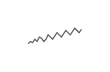
\begin{tikzpicture}[x=0.08em, y=0.08em, line width=0.4pt]
                \draw[FooterGray] (0,3) -- (1,4) -- (2,3.5) -- (3,5) -- (4,4) -- (5,6) -- (6,5.5) -- (7,4) -- (8,5) -- (9,7) -- (10,6) -- (11,5) -- (12,6.5) -- (13,8) -- (14,7) -- (15,6) -- (16,7.5) -- (17,9) -- (18,8) -- (19,7) -- (20,8.5) -- (21,10) -- (22,9) -- (23,8) -- (24,9.5);
            \end{tikzpicture}%
        }%
        \hskip0.5cm%
    }%
    \vskip6pt%
}

%=============================================================================
% PACKAGES
%=============================================================================
\usepackage[utf8]{inputenc}
\DeclareUnicodeCharacter{03B1}{\ensuremath{\alpha}}
\usepackage[T1]{fontenc}
\usepackage{amsmath, amssymb, amsthm}
\usepackage{mathtools}
\usepackage{bm}
\usepackage{tikz}
\usetikzlibrary{arrows.meta, positioning, shapes, calc, decorations.pathreplacing, shadings}
\usepackage{booktabs}
\usepackage{multirow}
\usepackage{array}
\usepackage{graphicx}
\usepackage{animate}
\usepackage{hyperref}
\usepackage{colortbl}
\usepackage{listings}
\lstset{language=Python, basicstyle=\ttfamily\scriptsize, keywordstyle=\color{MainBlue}\bfseries,
  commentstyle=\color{Forest}, stringstyle=\color{Crimson}, breaklines=true,
  frame=none, backgroundcolor=\color{VeryLightGray}, xleftmargin=2mm}
\hypersetup{colorlinks=true, linkcolor=MainBlue, urlcolor=MainBlue}
\graphicspath{{../../logos/}{../../charts/}{../../photos/}}
\usepackage{xcolor}
\hfuzz=2pt  % Suppress tiny overfull warnings (<2pt)
\vfuzz=2pt  % Suppress tiny vertical overfull warnings (<2pt)
% \mathrm in the sans-serif family of the slides (beamer resets \mathrm to the serif family at \begin{document};
% this hook runs after beamer's, so WN, Var, RMSE, ... in formulas match the surrounding text)
% Bold vectors and matrices in the same sans-serif family: \mathbf{A} in sans bold (beamer's own \mathbf came out in
% medium weight), and the bold upright Greek capitals of \boldsymbol / \bm (\bSigma, \bPhi, \boldsymbol{\Theta}) in
% cmss bold: bm.sty fixes its "boldoperators" font when it is loaded (serif cmbx), before beamer switches the
% operators to cmss, so it is reset here.
\AtBeginDocument{%
  \SetMathAlphabet{\mathrm}{normal}{\encodingdefault}{\sfdefault}{\mddefault}{n}%
  \SetMathAlphabet{\mathrm}{bold}{\encodingdefault}{\sfdefault}{bx}{n}%
  \SetMathAlphabet{\mathbf}{normal}{\encodingdefault}{\sfdefault}{bx}{n}%
  \SetMathAlphabet{\mathbf}{bold}{\encodingdefault}{\sfdefault}{bx}{n}%
  \SetSymbolFont{boldoperators}{normal}{OT1}{cmss}{bx}{n}%
  \SetSymbolFont{boldoperators}{bold}{OT1}{cmss}{bx}{n}}

%=============================================================================
% QUANTLET COMMANDS
%   \quantlet{<displayed name>}{<url>}       (generic, compatible with the older TSA decks)
%   \tsaquantlet{Ch_05}{TSA_ch5_garch}       -> https://github.com/danpele/Time-Series-Analysis/tree/main/Quantlets/Ch_05/TSA_ch5_garch
%   \qlurl{<folder>} is defined per chapter by the generator (Quantlets/Ch_NN/<folder>)
%=============================================================================
\newcommand{\tsarepo}{https://github.com/danpele/Time-Series-Analysis}
\newcommand{\tsaqlbase}{https://github.com/danpele/Time-Series-Analysis/tree/main/Quantlets}
\newcommand{\quantlet}[2]{%
    \hfill\href{#2}{%
        \raisebox{-0.15em}{
\includegraphics[height=0.7em]{ql_logo.png}}%
        \textcolor{MainBlue}{\tiny\ #1}%
    }%
}
\newcommand{\tsaquantlet}[2]{\quantlet{\detokenize{#2}}{\tsaqlbase/#1/#2}}

%=============================================================================
% NOTEBOOKS (Google Colab)
%   \colaburl{notebooks/EN/chapter5_seminar_notebook.ipynb} -> the Colab link of a file in the TSA repo
%   \nb: the chapter notebook (each seminar deck redefines it with \renewcommand)
%=============================================================================
\newcommand{\colaburl}[1]{https://colab.research.google.com/github/danpele/Time-Series-Analysis/blob/main/#1}
\newcommand{\nb}{https://colab.research.google.com/github/danpele/Time-Series-Analysis/tree/main/notebooks/EN}
\newcommand{\nbname}{notebooks/EN}

%=============================================================================
% SLIDE HELPERS (used by the generators; the same as in MFM)
%=============================================================================
% local font size for list bodies (the preamble forces \normalsize)
\newcommand{\itemsize}[1]{\setbeamertemplate{itemize/enumerate body begin}{#1}\setbeamertemplate{itemize/enumerate subbody begin}{#1}}
\newcommand{\intitle}[1]{{\hypersetup{urlcolor=white}#1}}   % white links inside coloured title bars
\newcommand{\imgcap}[1]{{\scriptsize #1}\\[0.5mm]}          % caption under a photo
\newcommand{\imgcredit}[2]{{\tiny\color{FooterGray}\href{#1}{#2}}}   % image credit: source URL, author/licence
\newcommand{\aiprompt}[1]{{\ttfamily\color{MainBlue}#1}}     % a prompt to an AI assistant

%=============================================================================
% SEMINARS: student version by default; the instructor wrapper *_solutions.tex sets \solutionstrue
%=============================================================================
\makeatletter\@ifundefined{ifsolutions}{\expandafter\newif\csname ifsolutions\endcsname}{}\makeatother
\newcommand{\solonly}[1]{\ifsolutions #1\fi}
\newcommand{\propsub}{\ifsolutions\else\framesubtitle{\ifdefined\tsalang Rezolvarea se discută la seminar\else Solution discussed in class\fi}\fi}

%=============================================================================
% APPENDIX AND CHAPTER LINKS (latex/appendix_links.py writes the calls; it also re-declares these
% macros before \begin{document}, so the decks compile with or without this preamble block)
%=============================================================================
\providecommand{\tsaapplink}[3]{\hypertarget{#2}{}\hyperlink{#1}{\beamergotobutton{#3}}}
\providecommand{\tsaappback}[2]{\begin{tikzpicture}[remember picture,overlay]\node[anchor=south east] at ([xshift=-3mm,yshift=7mm]current page.south east){\hyperlink{#1}{\beamerreturnbutton{#2}}};\end{tikzpicture}}
\providecommand{\tsachlink}[2]{\href{#1}{#2}}
\providecommand{\tsachlinkt}[2]{\href{#1}{\usebeamercolor[fg]{frametitle}#2}}

%=============================================================================
% QUANTINAR COMMAND: link către un curs Quantinar (subiecte avansate)
%=============================================================================
\newcommand{\quantinar}[2]{%
    \href{#2}{%
        \raisebox{-0.15em}{
\includegraphics[height=0.8em]{qr_logo.png}}%
        \textcolor{MainBlue}{\scriptsize\ #1}%
    }%
}

%=============================================================================
% CUSTOM TITLE PAGE
%=============================================================================
\defbeamertemplate*{title page}{hybrid}[1][]
{
    \vspace{0.2cm}
    % Logos row - top header (with clickable links)
    \begin{center}
        \href{https://www.ase.ro}{
\includegraphics[height=1.0cm]{ase_logo.png}}\hspace{0.3cm}%
        \href{https://theida.net}{
\includegraphics[height=1.0cm]{ida_logo.png}}\hspace{0.3cm}%
        \href{https://blockchain-research-center.com}{
\includegraphics[height=1.0cm]{brc_logo.png}}\hspace{0.3cm}%
        \href{https://www.ai4efin.ase.ro}{
\includegraphics[height=1.0cm]{ai4efin_logo.png}}\hspace{0.3cm}%
        \href{https://ipe.ro/new}{
\includegraphics[height=1.0cm]{acad_logo.png}}\hspace{0.3cm}%
        \href{https://www.digital-finance-msca.com}{
\includegraphics[height=1.0cm]{msca_logo.png}}%
    \end{center}

    \vspace{0.6cm}

    % Main title with Q logos on sides (with clickable links)
    \begin{center}
        \begin{minipage}{0.1\textwidth}
            \centering
            \href{https://quantlet.com}{
\includegraphics[height=1.1cm]{ql_logo.png}}
        \end{minipage}%
        \begin{minipage}{0.78\textwidth}
            \centering
            {\LARGE\bfseries\usebeamercolor[fg]{title}\inserttitle}

            \vspace{0.3cm}

            {\usebeamerfont{subtitle}\usebeamercolor[fg]{title}\insertsubtitle}
        \end{minipage}%
        \begin{minipage}{0.1\textwidth}
            \centering
            \href{https://quantinar.com}{
\includegraphics[height=1.1cm]{qr_logo.png}}
        \end{minipage}
    \end{center}

    \vspace{0.6cm}

    % Authors (left aligned)
    \hspace{0.5cm}{\usebeamerfont{author}\insertauthor}

    \vspace{0.3cm}

    % Institute/Affiliations (left aligned)
    \hspace{0.5cm}\begin{minipage}[t]{0.9\textwidth}
        \raggedright\small\insertinstitute
    \end{minipage}
}

%=============================================================================
% THEOREM ENVIRONMENTS
%=============================================================================
\theoremstyle{definition}
\setbeamertemplate{theorems}[numbered]
\ifdefined\tsalang
\newtheorem{defn}{Definiție}
\newtheorem{thm}{Teoremă}
\newtheorem{prop}{Propoziție}
\newtheorem{rmk}{Observație}
\else
\newtheorem{defn}{Definition}
\newtheorem{thm}{Theorem}
\newtheorem{prop}{Proposition}
\newtheorem{rmk}{Remark}
\fi

%=============================================================================
% CENTRED MINIPAGE (no extra vertical space)
%=============================================================================
\newenvironment{cminipage}[1]{%
    \par\noindent\hfill\begin{minipage}{#1}\ignorespaces
}{%
    \end{minipage}\hfill\null\par
}

%=============================================================================
% CUSTOM COMMANDS
%=============================================================================
\newcommand{\E}{\mathbb{E}}
\newcommand{\Var}{\text{Var}}
\newcommand{\Cov}{\text{Cov}}
\newcommand{\Corr}{\text{Corr}}
\newcommand{\R}{\mathbb{R}}
\newcommand{\N}{\mathbb{N}}
\newcommand{\Z}{\mathbb{Z}}
\newcommand{\B}{\mathbf{B}}
\newcommand{\imark}{\textcolor{MainBlue}{\textbullet}}
\newcommand{\RMSE}{\text{RMSE}}
\newcommand{\MAE}{\text{MAE}}
\newcommand{\MAPE}{\text{MAPE}}

% Boldface vector/matrix commands (VAR, VECM, state space; also used by the older TSA decks)
\newcommand{\bY}{\mathbf{Y}}
\newcommand{\bX}{\mathbf{X}}
\newcommand{\bA}{\mathbf{A}}
\newcommand{\bB}{\mathbf{B}}
\newcommand{\bepsilon}{\boldsymbol{\varepsilon}}
\newcommand{\bSigma}{\boldsymbol{\Sigma}}
\newcommand{\bPhi}{\boldsymbol{\Phi}}
\newcommand{\bGamma}{\boldsymbol{\Gamma}}
\newcommand{\bPi}{\boldsymbol{\Pi}}
\newcommand{\bc}{\mathbf{c}}
\newcommand{\balpha}{\boldsymbol{\alpha}}
\newcommand{\bbeta}{\boldsymbol{\beta}}
\newcommand{\bvarepsilon}{\boldsymbol{\varepsilon}}

% Legacy seminar marks (older TSA seminar decks)
\newcommand{\correct}{\textcolor{Forest}{\checkmark}}
\newcommand{\incorrect}{\textcolor{Crimson}{\texttimes}}
 se definește
%   \newcommand{\coursename}{Time Series Analysis}      (EN)
%   \newcommand{\coursename}{Serii de timp}       (RO)  și  \def\tsalang{ro}
% Fișierele .tex se află în EN/Courses, EN/Seminars, RO/Cursuri, RO/Seminarii (două niveluri sub rădăcină).
% Deck-urile sînt generate de latex/build_chapterN.py / build_seminarN.py (vezi latex/tsa_build.py).

\documentclass[9pt, aspectratio=169, t]{beamer}
\providecommand{\coursename}{Time Series Analysis}

% Ensure content fits on slides
\setbeamersize{text margin left=8mm, text margin right=8mm}
% Smaller institute font (title page)
\setbeamerfont{institute}{size=\footnotesize}

%=============================================================================
% THEME AND STYLE CONFIGURATION
%=============================================================================
\usetheme{default}
% Using default theme for clean header/footer control

% Color Palette (matching Redispatch PDF)
\definecolor{MainBlue}{RGB}{26, 58, 110}
\definecolor{AccentBlue}{RGB}{26, 58, 110}
\definecolor{IDAred}{RGB}{205, 0, 0}
\definecolor{DarkGray}{RGB}{51, 51, 51}
\definecolor{MediumGray}{RGB}{128, 128, 128}
\definecolor{LightGray}{RGB}{248, 248, 248}
\definecolor{VeryLightGray}{RGB}{235, 235, 235}
\definecolor{KeynoteGray}{RGB}{218, 218, 218}
\definecolor{SectionGray}{RGB}{120, 120, 120}
\definecolor{FooterGray}{RGB}{100, 100, 100}
\definecolor{Crimson}{RGB}{220, 53, 69}
\definecolor{Forest}{RGB}{46, 125, 50}
\definecolor{Amber}{RGB}{181, 133, 63}
\definecolor{Orange}{RGB}{230, 126, 34}
\definecolor{Purple}{RGB}{142, 68, 173}

% Gradient background (exact Keynote 315° gradient: white to RGB 218,218,218)
\setbeamertemplate{background}{%
    \begin{tikzpicture}[remember picture, overlay]
        \shade[shading=axis, shading angle=315,
        top color=white, bottom color=KeynoteGray]
        (current page.south west) rectangle (current page.north east);
    \end{tikzpicture}%
}
% Fallback solid color for compatibility
\setbeamercolor{background canvas}{bg=}

\setbeamercolor{palette primary}{bg=MainBlue, fg=white}
\setbeamercolor{palette secondary}{bg=MainBlue!85, fg=white}
\setbeamercolor{palette tertiary}{bg=MainBlue!70, fg=white}
\setbeamercolor{structure}{fg=MainBlue}
\setbeamercolor{title}{fg=IDAred}
\setbeamercolor{frametitle}{fg=IDAred, bg=}
\setbeamercolor{block title}{bg=MainBlue, fg=white}
\setbeamercolor{block body}{bg=VeryLightGray, fg=DarkGray}
\setbeamercolor{block title alerted}{bg=Crimson, fg=white}
\setbeamercolor{block body alerted}{bg=Crimson!8, fg=DarkGray}
\setbeamercolor{block title example}{bg=Forest, fg=white}
\setbeamercolor{block body example}{bg=Forest!8, fg=DarkGray}
\setbeamercolor{item}{fg=MainBlue}

% Footer colors (override Madrid theme blue)
\setbeamercolor{author in head/foot}{fg=FooterGray, bg=}
\setbeamercolor{title in head/foot}{fg=FooterGray, bg=}
\setbeamercolor{date in head/foot}{fg=FooterGray, bg=}
\setbeamercolor{section in head/foot}{fg=FooterGray, bg=}
\setbeamercolor{subsection in head/foot}{fg=FooterGray, bg=}

% Bullet styles (apply everywhere including blocks)
\setbeamertemplate{itemize item}{\color{MainBlue}$\boxdot$}
\setbeamertemplate{itemize subitem}{\color{MainBlue}$\blacktriangleright$}
\setbeamertemplate{itemize subsubitem}{\color{MainBlue}\tiny$\bullet$}
\setbeamertemplate{itemize/enumerate body begin}{\normalsize}
\setbeamertemplate{itemize/enumerate subbody begin}{\normalsize}

% Item spacing - compact style
\setlength{\leftmargini}{10pt}       % Level 1: minimal indent
\setlength{\leftmarginii}{10pt}      % Level 2: minimal additional indent
% Compact list spacing (zero extra space before/after lists in blocks)
\makeatletter
\def\@listi{\leftmargin\leftmargini \topsep 0pt \parsep 0pt \itemsep 0pt}
\def\@listii{\leftmargin\leftmarginii \topsep 0pt \parsep 0pt \itemsep 0pt}
\makeatother

\setbeamertemplate{navigation symbols}{}

%=============================================================================
% CUSTOM HEADLINE
%=============================================================================
\setbeamertemplate{headline}{%
    \vskip10pt%
    \hbox to \paperwidth{%
        \hskip0.5cm%
        {\small\color{FooterGray}\renewcommand{\hyperlink}[2]{##2}\insertsectionhead}%
        \hfill%
        \textcolor{FooterGray}{\small\insertframenumber}%
        \hskip0.5cm%
    }%
    \vskip4pt%
    {\color{FooterGray}\hrule height 0.4pt}%
}

%=============================================================================
% CUSTOM FOOTER
%=============================================================================
\usepackage{fontawesome5}

\setbeamertemplate{footline}{%
    {\color{FooterGray}\hrule height 0.4pt}%
    \vskip4pt%
    \hbox to \paperwidth{%
        \hskip0.5cm%
        \textcolor{FooterGray}{\small\coursename}%
        \hfill%
        \raisebox{-0.1em}{%
            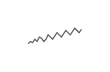
\begin{tikzpicture}[x=0.08em, y=0.08em, line width=0.4pt]
                \draw[FooterGray] (0,3) -- (1,4) -- (2,3.5) -- (3,5) -- (4,4) -- (5,6) -- (6,5.5) -- (7,4) -- (8,5) -- (9,7) -- (10,6) -- (11,5) -- (12,6.5) -- (13,8) -- (14,7) -- (15,6) -- (16,7.5) -- (17,9) -- (18,8) -- (19,7) -- (20,8.5) -- (21,10) -- (22,9) -- (23,8) -- (24,9.5);
            \end{tikzpicture}%
        }%
        \hskip0.5cm%
    }%
    \vskip6pt%
}

%=============================================================================
% PACKAGES
%=============================================================================
\usepackage[utf8]{inputenc}
\DeclareUnicodeCharacter{03B1}{\ensuremath{\alpha}}
\usepackage[T1]{fontenc}
\usepackage{amsmath, amssymb, amsthm}
\usepackage{mathtools}
\usepackage{bm}
\usepackage{tikz}
\usetikzlibrary{arrows.meta, positioning, shapes, calc, decorations.pathreplacing, shadings}
\usepackage{booktabs}
\usepackage{multirow}
\usepackage{array}
\usepackage{graphicx}
\usepackage{animate}
\usepackage{hyperref}
\usepackage{colortbl}
\usepackage{listings}
\lstset{language=Python, basicstyle=\ttfamily\scriptsize, keywordstyle=\color{MainBlue}\bfseries,
  commentstyle=\color{Forest}, stringstyle=\color{Crimson}, breaklines=true,
  frame=none, backgroundcolor=\color{VeryLightGray}, xleftmargin=2mm}
\hypersetup{colorlinks=true, linkcolor=MainBlue, urlcolor=MainBlue}
\graphicspath{{../../logos/}{../../charts/}{../../photos/}}
\usepackage{xcolor}
\hfuzz=2pt  % Suppress tiny overfull warnings (<2pt)
\vfuzz=2pt  % Suppress tiny vertical overfull warnings (<2pt)
% \mathrm in the sans-serif family of the slides (beamer resets \mathrm to the serif family at \begin{document};
% this hook runs after beamer's, so WN, Var, RMSE, ... in formulas match the surrounding text)
% Bold vectors and matrices in the same sans-serif family: \mathbf{A} in sans bold (beamer's own \mathbf came out in
% medium weight), and the bold upright Greek capitals of \boldsymbol / \bm (\bSigma, \bPhi, \boldsymbol{\Theta}) in
% cmss bold: bm.sty fixes its "boldoperators" font when it is loaded (serif cmbx), before beamer switches the
% operators to cmss, so it is reset here.
\AtBeginDocument{%
  \SetMathAlphabet{\mathrm}{normal}{\encodingdefault}{\sfdefault}{\mddefault}{n}%
  \SetMathAlphabet{\mathrm}{bold}{\encodingdefault}{\sfdefault}{bx}{n}%
  \SetMathAlphabet{\mathbf}{normal}{\encodingdefault}{\sfdefault}{bx}{n}%
  \SetMathAlphabet{\mathbf}{bold}{\encodingdefault}{\sfdefault}{bx}{n}%
  \SetSymbolFont{boldoperators}{normal}{OT1}{cmss}{bx}{n}%
  \SetSymbolFont{boldoperators}{bold}{OT1}{cmss}{bx}{n}}

%=============================================================================
% QUANTLET COMMANDS
%   \quantlet{<displayed name>}{<url>}       (generic, compatible with the older TSA decks)
%   \tsaquantlet{Ch_05}{TSA_ch5_garch}       -> https://github.com/danpele/Time-Series-Analysis/tree/main/Quantlets/Ch_05/TSA_ch5_garch
%   \qlurl{<folder>} is defined per chapter by the generator (Quantlets/Ch_NN/<folder>)
%=============================================================================
\newcommand{\tsarepo}{https://github.com/danpele/Time-Series-Analysis}
\newcommand{\tsaqlbase}{https://github.com/danpele/Time-Series-Analysis/tree/main/Quantlets}
\newcommand{\quantlet}[2]{%
    \hfill\href{#2}{%
        \raisebox{-0.15em}{
\includegraphics[height=0.7em]{ql_logo.png}}%
        \textcolor{MainBlue}{\tiny\ #1}%
    }%
}
\newcommand{\tsaquantlet}[2]{\quantlet{\detokenize{#2}}{\tsaqlbase/#1/#2}}

%=============================================================================
% NOTEBOOKS (Google Colab)
%   \colaburl{notebooks/EN/chapter5_seminar_notebook.ipynb} -> the Colab link of a file in the TSA repo
%   \nb: the chapter notebook (each seminar deck redefines it with \renewcommand)
%=============================================================================
\newcommand{\colaburl}[1]{https://colab.research.google.com/github/danpele/Time-Series-Analysis/blob/main/#1}
\newcommand{\nb}{https://colab.research.google.com/github/danpele/Time-Series-Analysis/tree/main/notebooks/EN}
\newcommand{\nbname}{notebooks/EN}

%=============================================================================
% SLIDE HELPERS (used by the generators; the same as in MFM)
%=============================================================================
% local font size for list bodies (the preamble forces \normalsize)
\newcommand{\itemsize}[1]{\setbeamertemplate{itemize/enumerate body begin}{#1}\setbeamertemplate{itemize/enumerate subbody begin}{#1}}
\newcommand{\intitle}[1]{{\hypersetup{urlcolor=white}#1}}   % white links inside coloured title bars
\newcommand{\imgcap}[1]{{\scriptsize #1}\\[0.5mm]}          % caption under a photo
\newcommand{\imgcredit}[2]{{\tiny\color{FooterGray}\href{#1}{#2}}}   % image credit: source URL, author/licence
\newcommand{\aiprompt}[1]{{\ttfamily\color{MainBlue}#1}}     % a prompt to an AI assistant

%=============================================================================
% SEMINARS: student version by default; the instructor wrapper *_solutions.tex sets \solutionstrue
%=============================================================================
\makeatletter\@ifundefined{ifsolutions}{\expandafter\newif\csname ifsolutions\endcsname}{}\makeatother
\newcommand{\solonly}[1]{\ifsolutions #1\fi}
\newcommand{\propsub}{\ifsolutions\else\framesubtitle{\ifdefined\tsalang Rezolvarea se discută la seminar\else Solution discussed in class\fi}\fi}

%=============================================================================
% APPENDIX AND CHAPTER LINKS (latex/appendix_links.py writes the calls; it also re-declares these
% macros before \begin{document}, so the decks compile with or without this preamble block)
%=============================================================================
\providecommand{\tsaapplink}[3]{\hypertarget{#2}{}\hyperlink{#1}{\beamergotobutton{#3}}}
\providecommand{\tsaappback}[2]{\begin{tikzpicture}[remember picture,overlay]\node[anchor=south east] at ([xshift=-3mm,yshift=7mm]current page.south east){\hyperlink{#1}{\beamerreturnbutton{#2}}};\end{tikzpicture}}
\providecommand{\tsachlink}[2]{\href{#1}{#2}}
\providecommand{\tsachlinkt}[2]{\href{#1}{\usebeamercolor[fg]{frametitle}#2}}

%=============================================================================
% QUANTINAR COMMAND: link către un curs Quantinar (subiecte avansate)
%=============================================================================
\newcommand{\quantinar}[2]{%
    \href{#2}{%
        \raisebox{-0.15em}{
\includegraphics[height=0.8em]{qr_logo.png}}%
        \textcolor{MainBlue}{\scriptsize\ #1}%
    }%
}

%=============================================================================
% CUSTOM TITLE PAGE
%=============================================================================
\defbeamertemplate*{title page}{hybrid}[1][]
{
    \vspace{0.2cm}
    % Logos row - top header (with clickable links)
    \begin{center}
        \href{https://www.ase.ro}{
\includegraphics[height=1.0cm]{ase_logo.png}}\hspace{0.3cm}%
        \href{https://theida.net}{
\includegraphics[height=1.0cm]{ida_logo.png}}\hspace{0.3cm}%
        \href{https://blockchain-research-center.com}{
\includegraphics[height=1.0cm]{brc_logo.png}}\hspace{0.3cm}%
        \href{https://www.ai4efin.ase.ro}{
\includegraphics[height=1.0cm]{ai4efin_logo.png}}\hspace{0.3cm}%
        \href{https://ipe.ro/new}{
\includegraphics[height=1.0cm]{acad_logo.png}}\hspace{0.3cm}%
        \href{https://www.digital-finance-msca.com}{
\includegraphics[height=1.0cm]{msca_logo.png}}%
    \end{center}

    \vspace{0.6cm}

    % Main title with Q logos on sides (with clickable links)
    \begin{center}
        \begin{minipage}{0.1\textwidth}
            \centering
            \href{https://quantlet.com}{
\includegraphics[height=1.1cm]{ql_logo.png}}
        \end{minipage}%
        \begin{minipage}{0.78\textwidth}
            \centering
            {\LARGE\bfseries\usebeamercolor[fg]{title}\inserttitle}

            \vspace{0.3cm}

            {\usebeamerfont{subtitle}\usebeamercolor[fg]{title}\insertsubtitle}
        \end{minipage}%
        \begin{minipage}{0.1\textwidth}
            \centering
            \href{https://quantinar.com}{
\includegraphics[height=1.1cm]{qr_logo.png}}
        \end{minipage}
    \end{center}

    \vspace{0.6cm}

    % Authors (left aligned)
    \hspace{0.5cm}{\usebeamerfont{author}\insertauthor}

    \vspace{0.3cm}

    % Institute/Affiliations (left aligned)
    \hspace{0.5cm}\begin{minipage}[t]{0.9\textwidth}
        \raggedright\small\insertinstitute
    \end{minipage}
}

%=============================================================================
% THEOREM ENVIRONMENTS
%=============================================================================
\theoremstyle{definition}
\setbeamertemplate{theorems}[numbered]
\ifdefined\tsalang
\newtheorem{defn}{Definiție}
\newtheorem{thm}{Teoremă}
\newtheorem{prop}{Propoziție}
\newtheorem{rmk}{Observație}
\else
\newtheorem{defn}{Definition}
\newtheorem{thm}{Theorem}
\newtheorem{prop}{Proposition}
\newtheorem{rmk}{Remark}
\fi

%=============================================================================
% CENTRED MINIPAGE (no extra vertical space)
%=============================================================================
\newenvironment{cminipage}[1]{%
    \par\noindent\hfill\begin{minipage}{#1}\ignorespaces
}{%
    \end{minipage}\hfill\null\par
}

%=============================================================================
% CUSTOM COMMANDS
%=============================================================================
\newcommand{\E}{\mathbb{E}}
\newcommand{\Var}{\text{Var}}
\newcommand{\Cov}{\text{Cov}}
\newcommand{\Corr}{\text{Corr}}
\newcommand{\R}{\mathbb{R}}
\newcommand{\N}{\mathbb{N}}
\newcommand{\Z}{\mathbb{Z}}
\newcommand{\B}{\mathbf{B}}
\newcommand{\imark}{\textcolor{MainBlue}{\textbullet}}
\newcommand{\RMSE}{\text{RMSE}}
\newcommand{\MAE}{\text{MAE}}
\newcommand{\MAPE}{\text{MAPE}}

% Boldface vector/matrix commands (VAR, VECM, state space; also used by the older TSA decks)
\newcommand{\bY}{\mathbf{Y}}
\newcommand{\bX}{\mathbf{X}}
\newcommand{\bA}{\mathbf{A}}
\newcommand{\bB}{\mathbf{B}}
\newcommand{\bepsilon}{\boldsymbol{\varepsilon}}
\newcommand{\bSigma}{\boldsymbol{\Sigma}}
\newcommand{\bPhi}{\boldsymbol{\Phi}}
\newcommand{\bGamma}{\boldsymbol{\Gamma}}
\newcommand{\bPi}{\boldsymbol{\Pi}}
\newcommand{\bc}{\mathbf{c}}
\newcommand{\balpha}{\boldsymbol{\alpha}}
\newcommand{\bbeta}{\boldsymbol{\beta}}
\newcommand{\bvarepsilon}{\boldsymbol{\varepsilon}}

% Legacy seminar marks (older TSA seminar decks)
\newcommand{\correct}{\textcolor{Forest}{\checkmark}}
\newcommand{\incorrect}{\textcolor{Crimson}{\texttimes}}
 se definește
%   \newcommand{\coursename}{Time Series Analysis}      (EN)
%   \newcommand{\coursename}{Serii de timp}       (RO)  și  \def\tsalang{ro}
% Fișierele .tex se află în EN/Courses, EN/Seminars, RO/Cursuri, RO/Seminarii (două niveluri sub rădăcină).
% Deck-urile sînt generate de latex/build_chapterN.py / build_seminarN.py (vezi latex/tsa_build.py).

\documentclass[9pt, aspectratio=169, t]{beamer}
\providecommand{\coursename}{Time Series Analysis}

% Ensure content fits on slides
\setbeamersize{text margin left=8mm, text margin right=8mm}
% Smaller institute font (title page)
\setbeamerfont{institute}{size=\footnotesize}

%=============================================================================
% THEME AND STYLE CONFIGURATION
%=============================================================================
\usetheme{default}
% Using default theme for clean header/footer control

% Color Palette (matching Redispatch PDF)
\definecolor{MainBlue}{RGB}{26, 58, 110}
\definecolor{AccentBlue}{RGB}{26, 58, 110}
\definecolor{IDAred}{RGB}{205, 0, 0}
\definecolor{DarkGray}{RGB}{51, 51, 51}
\definecolor{MediumGray}{RGB}{128, 128, 128}
\definecolor{LightGray}{RGB}{248, 248, 248}
\definecolor{VeryLightGray}{RGB}{235, 235, 235}
\definecolor{KeynoteGray}{RGB}{218, 218, 218}
\definecolor{SectionGray}{RGB}{120, 120, 120}
\definecolor{FooterGray}{RGB}{100, 100, 100}
\definecolor{Crimson}{RGB}{220, 53, 69}
\definecolor{Forest}{RGB}{46, 125, 50}
\definecolor{Amber}{RGB}{181, 133, 63}
\definecolor{Orange}{RGB}{230, 126, 34}
\definecolor{Purple}{RGB}{142, 68, 173}

% Gradient background (exact Keynote 315° gradient: white to RGB 218,218,218)
\setbeamertemplate{background}{%
    \begin{tikzpicture}[remember picture, overlay]
        \shade[shading=axis, shading angle=315,
        top color=white, bottom color=KeynoteGray]
        (current page.south west) rectangle (current page.north east);
    \end{tikzpicture}%
}
% Fallback solid color for compatibility
\setbeamercolor{background canvas}{bg=}

\setbeamercolor{palette primary}{bg=MainBlue, fg=white}
\setbeamercolor{palette secondary}{bg=MainBlue!85, fg=white}
\setbeamercolor{palette tertiary}{bg=MainBlue!70, fg=white}
\setbeamercolor{structure}{fg=MainBlue}
\setbeamercolor{title}{fg=IDAred}
\setbeamercolor{frametitle}{fg=IDAred, bg=}
\setbeamercolor{block title}{bg=MainBlue, fg=white}
\setbeamercolor{block body}{bg=VeryLightGray, fg=DarkGray}
\setbeamercolor{block title alerted}{bg=Crimson, fg=white}
\setbeamercolor{block body alerted}{bg=Crimson!8, fg=DarkGray}
\setbeamercolor{block title example}{bg=Forest, fg=white}
\setbeamercolor{block body example}{bg=Forest!8, fg=DarkGray}
\setbeamercolor{item}{fg=MainBlue}

% Footer colors (override Madrid theme blue)
\setbeamercolor{author in head/foot}{fg=FooterGray, bg=}
\setbeamercolor{title in head/foot}{fg=FooterGray, bg=}
\setbeamercolor{date in head/foot}{fg=FooterGray, bg=}
\setbeamercolor{section in head/foot}{fg=FooterGray, bg=}
\setbeamercolor{subsection in head/foot}{fg=FooterGray, bg=}

% Bullet styles (apply everywhere including blocks)
\setbeamertemplate{itemize item}{\color{MainBlue}$\boxdot$}
\setbeamertemplate{itemize subitem}{\color{MainBlue}$\blacktriangleright$}
\setbeamertemplate{itemize subsubitem}{\color{MainBlue}\tiny$\bullet$}
\setbeamertemplate{itemize/enumerate body begin}{\normalsize}
\setbeamertemplate{itemize/enumerate subbody begin}{\normalsize}

% Item spacing - compact style
\setlength{\leftmargini}{10pt}       % Level 1: minimal indent
\setlength{\leftmarginii}{10pt}      % Level 2: minimal additional indent
% Compact list spacing (zero extra space before/after lists in blocks)
\makeatletter
\def\@listi{\leftmargin\leftmargini \topsep 0pt \parsep 0pt \itemsep 0pt}
\def\@listii{\leftmargin\leftmarginii \topsep 0pt \parsep 0pt \itemsep 0pt}
\makeatother

\setbeamertemplate{navigation symbols}{}

%=============================================================================
% CUSTOM HEADLINE
%=============================================================================
\setbeamertemplate{headline}{%
    \vskip10pt%
    \hbox to \paperwidth{%
        \hskip0.5cm%
        {\small\color{FooterGray}\renewcommand{\hyperlink}[2]{##2}\insertsectionhead}%
        \hfill%
        \textcolor{FooterGray}{\small\insertframenumber}%
        \hskip0.5cm%
    }%
    \vskip4pt%
    {\color{FooterGray}\hrule height 0.4pt}%
}

%=============================================================================
% CUSTOM FOOTER
%=============================================================================
\usepackage{fontawesome5}

\setbeamertemplate{footline}{%
    {\color{FooterGray}\hrule height 0.4pt}%
    \vskip4pt%
    \hbox to \paperwidth{%
        \hskip0.5cm%
        \textcolor{FooterGray}{\small\coursename}%
        \hfill%
        \raisebox{-0.1em}{%
            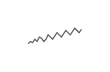
\begin{tikzpicture}[x=0.08em, y=0.08em, line width=0.4pt]
                \draw[FooterGray] (0,3) -- (1,4) -- (2,3.5) -- (3,5) -- (4,4) -- (5,6) -- (6,5.5) -- (7,4) -- (8,5) -- (9,7) -- (10,6) -- (11,5) -- (12,6.5) -- (13,8) -- (14,7) -- (15,6) -- (16,7.5) -- (17,9) -- (18,8) -- (19,7) -- (20,8.5) -- (21,10) -- (22,9) -- (23,8) -- (24,9.5);
            \end{tikzpicture}%
        }%
        \hskip0.5cm%
    }%
    \vskip6pt%
}

%=============================================================================
% PACKAGES
%=============================================================================
\usepackage[utf8]{inputenc}
\DeclareUnicodeCharacter{03B1}{\ensuremath{\alpha}}
\usepackage[T1]{fontenc}
\usepackage{amsmath, amssymb, amsthm}
\usepackage{mathtools}
\usepackage{bm}
\usepackage{tikz}
\usetikzlibrary{arrows.meta, positioning, shapes, calc, decorations.pathreplacing, shadings}
\usepackage{booktabs}
\usepackage{multirow}
\usepackage{array}
\usepackage{graphicx}
\usepackage{animate}
\usepackage{hyperref}
\usepackage{colortbl}
\usepackage{listings}
\lstset{language=Python, basicstyle=\ttfamily\scriptsize, keywordstyle=\color{MainBlue}\bfseries,
  commentstyle=\color{Forest}, stringstyle=\color{Crimson}, breaklines=true,
  frame=none, backgroundcolor=\color{VeryLightGray}, xleftmargin=2mm}
\hypersetup{colorlinks=true, linkcolor=MainBlue, urlcolor=MainBlue}
\graphicspath{{../../logos/}{../../charts/}{../../photos/}}
\usepackage{xcolor}
\hfuzz=2pt  % Suppress tiny overfull warnings (<2pt)
\vfuzz=2pt  % Suppress tiny vertical overfull warnings (<2pt)
% \mathrm in the sans-serif family of the slides (beamer resets \mathrm to the serif family at \begin{document};
% this hook runs after beamer's, so WN, Var, RMSE, ... in formulas match the surrounding text)
% Bold vectors and matrices in the same sans-serif family: \mathbf{A} in sans bold (beamer's own \mathbf came out in
% medium weight), and the bold upright Greek capitals of \boldsymbol / \bm (\bSigma, \bPhi, \boldsymbol{\Theta}) in
% cmss bold: bm.sty fixes its "boldoperators" font when it is loaded (serif cmbx), before beamer switches the
% operators to cmss, so it is reset here.
\AtBeginDocument{%
  \SetMathAlphabet{\mathrm}{normal}{\encodingdefault}{\sfdefault}{\mddefault}{n}%
  \SetMathAlphabet{\mathrm}{bold}{\encodingdefault}{\sfdefault}{bx}{n}%
  \SetMathAlphabet{\mathbf}{normal}{\encodingdefault}{\sfdefault}{bx}{n}%
  \SetMathAlphabet{\mathbf}{bold}{\encodingdefault}{\sfdefault}{bx}{n}%
  \SetSymbolFont{boldoperators}{normal}{OT1}{cmss}{bx}{n}%
  \SetSymbolFont{boldoperators}{bold}{OT1}{cmss}{bx}{n}}

%=============================================================================
% QUANTLET COMMANDS
%   \quantlet{<displayed name>}{<url>}       (generic, compatible with the older TSA decks)
%   \tsaquantlet{Ch_05}{TSA_ch5_garch}       -> https://github.com/danpele/Time-Series-Analysis/tree/main/Quantlets/Ch_05/TSA_ch5_garch
%   \qlurl{<folder>} is defined per chapter by the generator (Quantlets/Ch_NN/<folder>)
%=============================================================================
\newcommand{\tsarepo}{https://github.com/danpele/Time-Series-Analysis}
\newcommand{\tsaqlbase}{https://github.com/danpele/Time-Series-Analysis/tree/main/Quantlets}
\newcommand{\quantlet}[2]{%
    \hfill\href{#2}{%
        \raisebox{-0.15em}{
\includegraphics[height=0.7em]{ql_logo.png}}%
        \textcolor{MainBlue}{\tiny\ #1}%
    }%
}
\newcommand{\tsaquantlet}[2]{\quantlet{\detokenize{#2}}{\tsaqlbase/#1/#2}}

%=============================================================================
% NOTEBOOKS (Google Colab)
%   \colaburl{notebooks/EN/chapter5_seminar_notebook.ipynb} -> the Colab link of a file in the TSA repo
%   \nb: the chapter notebook (each seminar deck redefines it with \renewcommand)
%=============================================================================
\newcommand{\colaburl}[1]{https://colab.research.google.com/github/danpele/Time-Series-Analysis/blob/main/#1}
\newcommand{\nb}{https://colab.research.google.com/github/danpele/Time-Series-Analysis/tree/main/notebooks/EN}
\newcommand{\nbname}{notebooks/EN}

%=============================================================================
% SLIDE HELPERS (used by the generators; the same as in MFM)
%=============================================================================
% local font size for list bodies (the preamble forces \normalsize)
\newcommand{\itemsize}[1]{\setbeamertemplate{itemize/enumerate body begin}{#1}\setbeamertemplate{itemize/enumerate subbody begin}{#1}}
\newcommand{\intitle}[1]{{\hypersetup{urlcolor=white}#1}}   % white links inside coloured title bars
\newcommand{\imgcap}[1]{{\scriptsize #1}\\[0.5mm]}          % caption under a photo
\newcommand{\imgcredit}[2]{{\tiny\color{FooterGray}\href{#1}{#2}}}   % image credit: source URL, author/licence
\newcommand{\aiprompt}[1]{{\ttfamily\color{MainBlue}#1}}     % a prompt to an AI assistant

%=============================================================================
% SEMINARS: student version by default; the instructor wrapper *_solutions.tex sets \solutionstrue
%=============================================================================
\makeatletter\@ifundefined{ifsolutions}{\expandafter\newif\csname ifsolutions\endcsname}{}\makeatother
\newcommand{\solonly}[1]{\ifsolutions #1\fi}
\newcommand{\propsub}{\ifsolutions\else\framesubtitle{\ifdefined\tsalang Rezolvarea se discută la seminar\else Solution discussed in class\fi}\fi}

%=============================================================================
% APPENDIX AND CHAPTER LINKS (latex/appendix_links.py writes the calls; it also re-declares these
% macros before \begin{document}, so the decks compile with or without this preamble block)
%=============================================================================
\providecommand{\tsaapplink}[3]{\hypertarget{#2}{}\hyperlink{#1}{\beamergotobutton{#3}}}
\providecommand{\tsaappback}[2]{\begin{tikzpicture}[remember picture,overlay]\node[anchor=south east] at ([xshift=-3mm,yshift=7mm]current page.south east){\hyperlink{#1}{\beamerreturnbutton{#2}}};\end{tikzpicture}}
\providecommand{\tsachlink}[2]{\href{#1}{#2}}
\providecommand{\tsachlinkt}[2]{\href{#1}{\usebeamercolor[fg]{frametitle}#2}}

%=============================================================================
% QUANTINAR COMMAND: link către un curs Quantinar (subiecte avansate)
%=============================================================================
\newcommand{\quantinar}[2]{%
    \href{#2}{%
        \raisebox{-0.15em}{
\includegraphics[height=0.8em]{qr_logo.png}}%
        \textcolor{MainBlue}{\scriptsize\ #1}%
    }%
}

%=============================================================================
% CUSTOM TITLE PAGE
%=============================================================================
\defbeamertemplate*{title page}{hybrid}[1][]
{
    \vspace{0.2cm}
    % Logos row - top header (with clickable links)
    \begin{center}
        \href{https://www.ase.ro}{
\includegraphics[height=1.0cm]{ase_logo.png}}\hspace{0.3cm}%
        \href{https://theida.net}{
\includegraphics[height=1.0cm]{ida_logo.png}}\hspace{0.3cm}%
        \href{https://blockchain-research-center.com}{
\includegraphics[height=1.0cm]{brc_logo.png}}\hspace{0.3cm}%
        \href{https://www.ai4efin.ase.ro}{
\includegraphics[height=1.0cm]{ai4efin_logo.png}}\hspace{0.3cm}%
        \href{https://ipe.ro/new}{
\includegraphics[height=1.0cm]{acad_logo.png}}\hspace{0.3cm}%
        \href{https://www.digital-finance-msca.com}{
\includegraphics[height=1.0cm]{msca_logo.png}}%
    \end{center}

    \vspace{0.6cm}

    % Main title with Q logos on sides (with clickable links)
    \begin{center}
        \begin{minipage}{0.1\textwidth}
            \centering
            \href{https://quantlet.com}{
\includegraphics[height=1.1cm]{ql_logo.png}}
        \end{minipage}%
        \begin{minipage}{0.78\textwidth}
            \centering
            {\LARGE\bfseries\usebeamercolor[fg]{title}\inserttitle}

            \vspace{0.3cm}

            {\usebeamerfont{subtitle}\usebeamercolor[fg]{title}\insertsubtitle}
        \end{minipage}%
        \begin{minipage}{0.1\textwidth}
            \centering
            \href{https://quantinar.com}{
\includegraphics[height=1.1cm]{qr_logo.png}}
        \end{minipage}
    \end{center}

    \vspace{0.6cm}

    % Authors (left aligned)
    \hspace{0.5cm}{\usebeamerfont{author}\insertauthor}

    \vspace{0.3cm}

    % Institute/Affiliations (left aligned)
    \hspace{0.5cm}\begin{minipage}[t]{0.9\textwidth}
        \raggedright\small\insertinstitute
    \end{minipage}
}

%=============================================================================
% THEOREM ENVIRONMENTS
%=============================================================================
\theoremstyle{definition}
\setbeamertemplate{theorems}[numbered]
\ifdefined\tsalang
\newtheorem{defn}{Definiție}
\newtheorem{thm}{Teoremă}
\newtheorem{prop}{Propoziție}
\newtheorem{rmk}{Observație}
\else
\newtheorem{defn}{Definition}
\newtheorem{thm}{Theorem}
\newtheorem{prop}{Proposition}
\newtheorem{rmk}{Remark}
\fi

%=============================================================================
% CENTRED MINIPAGE (no extra vertical space)
%=============================================================================
\newenvironment{cminipage}[1]{%
    \par\noindent\hfill\begin{minipage}{#1}\ignorespaces
}{%
    \end{minipage}\hfill\null\par
}

%=============================================================================
% CUSTOM COMMANDS
%=============================================================================
\newcommand{\E}{\mathbb{E}}
\newcommand{\Var}{\text{Var}}
\newcommand{\Cov}{\text{Cov}}
\newcommand{\Corr}{\text{Corr}}
\newcommand{\R}{\mathbb{R}}
\newcommand{\N}{\mathbb{N}}
\newcommand{\Z}{\mathbb{Z}}
\newcommand{\B}{\mathbf{B}}
\newcommand{\imark}{\textcolor{MainBlue}{\textbullet}}
\newcommand{\RMSE}{\text{RMSE}}
\newcommand{\MAE}{\text{MAE}}
\newcommand{\MAPE}{\text{MAPE}}

% Boldface vector/matrix commands (VAR, VECM, state space; also used by the older TSA decks)
\newcommand{\bY}{\mathbf{Y}}
\newcommand{\bX}{\mathbf{X}}
\newcommand{\bA}{\mathbf{A}}
\newcommand{\bB}{\mathbf{B}}
\newcommand{\bepsilon}{\boldsymbol{\varepsilon}}
\newcommand{\bSigma}{\boldsymbol{\Sigma}}
\newcommand{\bPhi}{\boldsymbol{\Phi}}
\newcommand{\bGamma}{\boldsymbol{\Gamma}}
\newcommand{\bPi}{\boldsymbol{\Pi}}
\newcommand{\bc}{\mathbf{c}}
\newcommand{\balpha}{\boldsymbol{\alpha}}
\newcommand{\bbeta}{\boldsymbol{\beta}}
\newcommand{\bvarepsilon}{\boldsymbol{\varepsilon}}

% Legacy seminar marks (older TSA seminar decks)
\newcommand{\correct}{\textcolor{Forest}{\checkmark}}
\newcommand{\incorrect}{\textcolor{Crimson}{\texttimes}}


\newcommand{\qlurl}[1]{https://github.com/danpele/Time-Series-Analysis/tree/main/Quantlets/Ch_08/#1}

% Clickable citations (DOIs verified via Crossref)
\newcommand{\refHP}{\href{https://doi.org/10.1007/978-3-031-13584-2}{Huang și Petukhina (2022)}}
\newcommand{\refBDtm}{\href{https://doi.org/10.1007/978-1-4419-0320-4}{Brockwell și Davis (1991)}}
\newcommand{\refBeran}{\href{https://doi.org/10.1007/978-3-642-35512-7}{Beran et al.\ (2013)}}
\newcommand{\refBaillie}{\href{https://doi.org/10.1016/0304-4076(95)01732-1}{Baillie (1996)}}
\newcommand{\refGraves}{\href{https://doi.org/10.3390/e19090437}{Graves et al.\ (2017)}}
\newcommand{\refHurst}{\href{https://doi.org/10.1061/TACEAT.0006518}{Hurst (1951)}}
\newcommand{\refMVN}{\href{https://doi.org/10.1137/1010093}{Mandelbrot și Van Ness (1968)}}
\newcommand{\refNoah}{\href{https://doi.org/10.1029/WR004i005p00909}{Mandelbrot și Wallis (1968)}}
\newcommand{\refMW}{\href{https://doi.org/10.1029/WR005i005p00967}{Mandelbrot și Wallis (1969)}}
\newcommand{\refGJ}{\href{https://doi.org/10.1111/j.1467-9892.1980.tb00297.x}{Granger și Joyeux (1980)}}
\newcommand{\refHosking}{\href{https://doi.org/10.1093/biomet/68.1.165}{Hosking (1981)}}
\newcommand{\refLo}{\href{https://doi.org/10.2307/2938368}{Lo (1991)}}
\newcommand{\refPeng}{\href{https://doi.org/10.1103/PhysRevE.49.1685}{Peng et al.\ (1994)}}
\newcommand{\refGPH}{\href{https://doi.org/10.1111/j.1467-9892.1983.tb00371.x}{Geweke și Porter-Hudak (1983)}}
\newcommand{\refRob}{\href{https://doi.org/10.1214/aos/1176324317}{Robinson (1995)}}
\newcommand{\refVelasco}{\href{https://doi.org/10.1111/1467-9892.00127}{Velasco (1999)}}
\newcommand{\refSowell}{\href{https://doi.org/10.1016/0304-4076(92)90084-5}{Sowell (1992)}}
\newcommand{\refFT}{\href{https://doi.org/10.1214/aos/1176349936}{Fox și Taqqu (1986)}}
\newcommand{\refRay}{\href{https://doi.org/10.1111/j.1467-9892.1993.tb00161.x}{Ray (1993)}}
\newcommand{\refHW}{\href{https://doi.org/10.1080/07350015.1995.10524577}{Hassler și Wolters (1995)}}
\newcommand{\refDGE}{\href{https://doi.org/10.1016/0927-5398(93)90006-D}{Ding, Granger și Engle (1993)}}
\newcommand{\refBBM}{\href{https://doi.org/10.1016/S0304-4076(95)01749-6}{Baillie, Bollerslev și Mikkelsen (1996)}}
\newcommand{\refABDL}{\href{https://doi.org/10.1111/1468-0262.00418}{Andersen et al.\ (2003)}}
\newcommand{\refCorsi}{\href{https://doi.org/10.1093/jjfinec/nbp001}{Corsi (2009)}}
\newcommand{\refDI}{\href{https://doi.org/10.1016/S0304-4076(01)00073-2}{Diebold și Inoue (2001)}}
\newcommand{\refGH}{\href{https://doi.org/10.1016/j.jempfin.2003.03.001}{Granger și Hyung (2004)}}
\newcommand{\refCobb}{\href{https://doi.org/10.1093/biomet/65.2.243}{Cobb (1978)}}
\newcommand{\refWeron}{\href{https://doi.org/10.1016/S0378-4371(02)00961-5}{Weron (2002)}}
\newcommand{\refCL}{\href{https://doi.org/10.1080/07350015.1993.10509936}{Cheung și Lai (1993)}}

\title[Serii de timp]{Serii de timp}
\subtitle{Capitolul 8: Memorie lungă și ARFIMA}
\author[D.T. Pele]{Daniel Traian PELE}
\institute{Academia de Studii Economice din București\\
IDA Institute Digital Assets\\
Blockchain Research Center\\
AI4EFin Artificial Intelligence for Energy Finance\\
Academia Română, Institutul de Prognoză Economică\\
MSCA Digital Finance}
\date{}

%=============================================================================
\providecommand{\tsaapplink}[3]{\hypertarget{#2}{}\hyperlink{#1}{\beamergotobutton{#3}}}  % APPLINKS-MACROS
\providecommand{\tsaappback}[2]{\begin{tikzpicture}[remember picture,overlay]\node[anchor=south east] at ([xshift=-3mm,yshift=7mm]current page.south east){\hyperlink{#1}{\beamerreturnbutton{#2}}};\end{tikzpicture}}  % APPLINKS-MACROS
\providecommand{\tsachlink}[2]{\href{#1}{#2}}  % APPLINKS-MACROS
\providecommand{\tsachlinkt}[2]{\href{#1}{\usebeamercolor[fg]{frametitle}#2}}  % APPLINKS-MACROS
\begin{document}
%=============================================================================

{
\setbeamertemplate{headline}{}
\setbeamertemplate{footline}{}
\begin{frame}[noframenumbering]
    \titlepage
\end{frame}
}
% BEGIN-ACRONYMS (generat de latex/acronyms.py; nu editati manual)
\begin{frame}{Acronime folosite în acest material (1/2)}
\setbeamertemplate{itemize/enumerate body begin}{\tiny}
\begin{columns}[T]
\begin{column}{0.49\textwidth}
\begin{itemize}\setlength{\itemsep}{0pt}
    \item \textbf{ACF}: Autocorrelation Function (funcția de autocorelație)
    \item \textbf{ADF}: Augmented Dickey–Fuller (test) — testul Dickey–Fuller augmentat
    \item \textbf{AI}: Artificial Intelligence (inteligență artificială)
    \item \textbf{AIC}: Akaike Information Criterion (criteriul informațional Akaike)
    \item \textbf{AR}: AutoRegressive (model); in event studies: Abnormal Return (model autoregresiv; în studiile de eveniment: randament anormal)
    \item \textbf{ARCH}: AutoRegressive Conditional Heteroskedasticity (heteroscedasticitate condiționată autoregresivă)
    \item \textbf{ARFIMA}: AutoRegressive Fractionally Integrated Moving Average (model) — model autoregresiv fracționar integrat cu medie mobilă
    \item \textbf{ARIMA}: AutoRegressive Integrated Moving Average (model) — model autoregresiv integrat cu medie mobilă
    \item \textbf{ARMA}: AutoRegressive Moving Average (model) — model autoregresiv cu medie mobilă
    \item \textbf{BET}: Bucharest Exchange Trading (index) — indicele de referință al Bursei de Valori București
    \item \textbf{BIC}: Bayesian Information Criterion (criteriul informațional bayesian (Schwarz))
    \item \textbf{BNR}: Banca Națională a României
    \item \textbf{CPIAUCSL}: Consumer Price Index for All Urban Consumers (FRED series code) — codul FRED al indicelui prețurilor de consum din SUA
\end{itemize}
\end{column}
\begin{column}{0.49\textwidth}
\begin{itemize}\setlength{\itemsep}{0pt}
    \item \textbf{DFA}: Detrended Fluctuation Analysis (analiza fluctuațiilor fără tendință)
    \item \textbf{EODHD}: EOD Historical Data (market-data provider) — furnizor de date de piață
    \item \textbf{FFT}: Fast Fourier Transform (transformata Fourier rapidă)
    \item \textbf{FIGARCH}: Fractionally Integrated GARCH (model GARCH fracționar integrat)
    \item \textbf{FRED}: Federal Reserve Economic Data (baza de date economice a Rezervei Federale din St. Louis)
    \item \textbf{GARCH}: Generalised AutoRegressive Conditional Heteroskedasticity (heteroscedasticitate condiționată autoregresivă generalizată)
    \item \textbf{GPH}: Geweke–Porter-Hudak (estimator) — estimatorul Geweke–Porter-Hudak al parametrului de memorie lungă
    \item \textbf{HAR}: Heterogeneous AutoRegressive (model) — model autoregresiv heterogen
    \item \textbf{HICP}: Harmonised Index of Consumer Prices (indicele armonizat al prețurilor de consum)
    \item \textbf{IAPC}: Indicele armonizat al prețurilor de consum
    \item \textbf{IGARCH}: Integrated GARCH (GARCH integrat)
    \item \textbf{IPC}: Indicele prețurilor de consum
    \item \textbf{MA}: Moving Average (medie mobilă)
\end{itemize}
\end{column}
\end{columns}
\end{frame}
\begin{frame}{Acronime folosite în acest material (2/2)}
\setbeamertemplate{itemize/enumerate body begin}{\tiny}
\begin{columns}[T]
\begin{column}{0.49\textwidth}
\begin{itemize}\setlength{\itemsep}{0pt}
    \item \textbf{ML}: Machine Learning (învățare automată)
    \item \textbf{OLS}: Ordinary Least Squares (metoda celor mai mici pătrate)
    \item \textbf{RMS}: Root Mean Square (abaterea medie pătratică)
    \item \textbf{RMSE}: Root Mean Squared Error (rădăcina erorii pătratice medii)
    \item \textbf{RV}: Realised Volatility (volatilitatea realizată)
    \item \textbf{SE}: Standard Error (eroare standard)
    \item \textbf{SUA}: Statele Unite ale Americii
    \item \textbf{UNRATE}: Unemployment Rate (FRED series code) — codul FRED al ratei șomajului din SUA
\end{itemize}
\end{column}
\begin{column}{0.49\textwidth}
\end{column}
\end{columns}
\end{frame}
% END-ACRONYMS

\begin{frame}{Întrebarea de azi și traseul}
\itemsize{\small}
\begin{itemize}
    \item \textbf{Întrebarea}: cît timp rămîne un șoc într-o serie? Modelele ARMA (\tsachlink{https://danpele.github.io/Time-Series-Analysis/RO/Cursuri/capitol2_modele_arma.pdf}{Capitolul 2}) uită exponențial; unele serii uită mult mai lent
    \begin{itemize}
        \item exemple: viiturile Nilului, inflația, șomajul, volatilitatea randamentelor bursiere
    \end{itemize}
    \item \textbf{Traseul} capitolului
    \begin{itemize}
        \item memorie scurtă și memorie lungă: descreșterea exponențială și cea hiperbolică a ACF
        \item diferențierea fracționară $(1-L)^d$ și modelul ARFIMA$(p,d,q)$
        \item estimarea lui $d$: R/S, DFA, GPH, Whittle local, verosimilitate maximă; prognoza
        \item memoria lungă a volatilității; memoria lungă aparentă, produsă de rupturi și regimuri
    \end{itemize}
    \item Pornim de la \tsachlink{https://danpele.github.io/Time-Series-Analysis/RO/Cursuri/capitol1_procese_stochastice_stationaritate.pdf}{Capitolul 1} (ACF, spectru), \tsachlink{https://danpele.github.io/Time-Series-Analysis/RO/Cursuri/capitol3_radacini_unitare_modele_arima.pdf}{Capitolul 3} (rădăcini unitare) și \tsachlink{https://danpele.github.io/Time-Series-Analysis/RO/Cursuri/capitol5_volatilitate_conditionata_garch.pdf}{Capitolul 5} (GARCH); Seminarul 8 are loc înaintea acestui curs
\end{itemize}
\end{frame}

\begin{frame}{Rezultatele învățării}
\itemsize{\small}
\begin{itemize}
    \item Distingeți memoria scurtă de memoria lungă după descreșterea ACF și după spectrul din apropierea frecvenței zero
    \item Calculați ponderile lui $(1-L)^d$ și autocorelațiile unui ARFIMA$(0,d,0)$
    \item Precizați intervalele de staționaritate și de inversabilitate ale lui $d$ și legătura $H = d + 1/2$
    \item Estimați $d$ cu R/S, DFA, GPH, Whittle local și verosimilitate maximă și apreciați incertitudinea estimărilor
    \item Faceți prognoze cu ARFIMA și comparați-le corect cu modele ARMA de referință
    \item Recunoașteți memoria lungă aparentă, cauzată de rupturi și de schimbări de regim
\end{itemize}
\end{frame}

\begin{frame}{Bibliografie și instrumente}
\itemsize{\small}
\begin{itemize}
    \item Manual: \refHP\ (modelele ARIMA și GARCH, pe care se sprijină acest capitol)
    \begin{itemize}
        \item teorie: \refBDtm, secț.~13.2 (procese cu memorie lungă); \refBeran; sinteză: \refBaillie
        \item istorie: \refGraves, „A brief history of long memory: Hurst, Mandelbrot and the road to ARFIMA”
    \end{itemize}
    \item Quantlet-urile Python ale capitolului: \href{https://github.com/danpele/Time-Series-Analysis/tree/main/Quantlets/Ch_08}{Quantlets/Ch\_08}
    \begin{itemize}
        \item estimatorii sînt scriși explicit în cod (R/S, DFA, GPH, Whittle local, ML exactă); \texttt{statsmodels} nu are o clasă ARFIMA; FIGARCH provine din pachetul \texttt{arch}
    \end{itemize}
    \item Notebook-ul cursului: \href{\colaburl{notebooks/EN/chapter8_lecture_notebook.ipynb}}{deschideți în Google Colab}
    \item Curs video: \quantinar{Applied Time Series Analysis with Python}{https://quantinar.com/course/137/applied-time-series-analysis-with-python}
\end{itemize}
\end{frame}


%=============================================================================
\section{Memorie scurtă și memorie lungă}
%=============================================================================

\begin{frame}{Harold Edwin Hurst și Nilul}
\itemsize{\footnotesize}
\begin{columns}[T]
\begin{column}{0.38\textwidth}
\centering
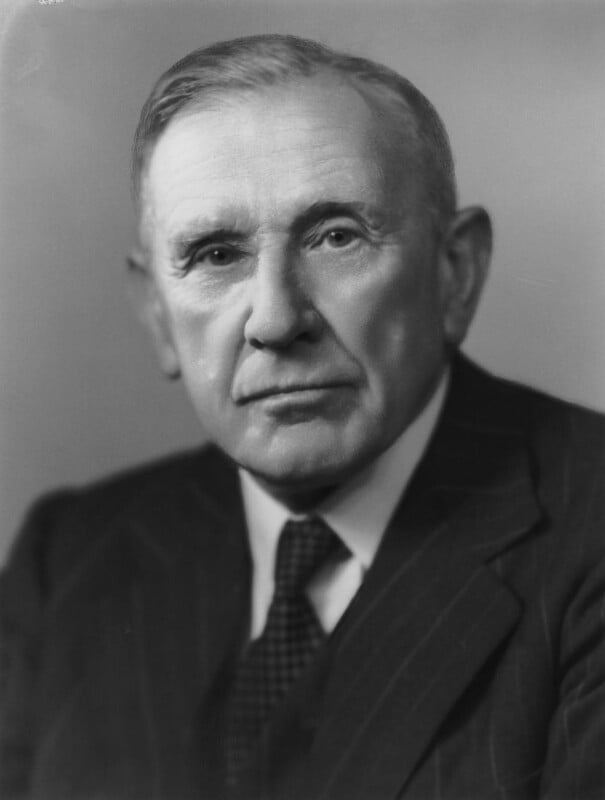
\includegraphics[height=0.38\textheight]{ch8_hurst_1953.jpg}\\[1mm]
\imgcap{H. E. Hurst (1880--1978)}
\imgcredit{https://commons.wikimedia.org/wiki/File:Harold_Edwin_Hurst_in_1953.jpg}{Foto: Elliott \& Fry (1953); domeniu public; Wikimedia Commons}
\end{column}
\begin{column}{0.6\textwidth}
\begin{itemize}
    \item Hurst a lucrat peste 60 de ani în Egipt, măsurînd Nilul pentru a dimensiona rezervoarele barajelor de la Aswan
    \begin{itemize}
        \item un rezervor trebuie să acopere cel mai lung șir de ani secetoși: mărimea lui depinde de \textbf{amplitudinea} intrărilor cumulate
    \end{itemize}
    \item \refHurst: amplitudinea crește ca $n^{H}$, cu $H \approx 0{,}7$, nu ca $n^{0{,}5}$, cum ar fi pentru ani independenți
    \begin{itemize}
        \item anii ploioși se grupează cu anii ploioși și cei secetoși cu cei secetoși, pe decenii: „efectul Iosif” din \refNoah
    \end{itemize}
    \item Aceasta este \textbf{memoria lungă}: o dependență care se stinge prea lent pentru orice model ARMA de ordin mic
\end{itemize}\centering
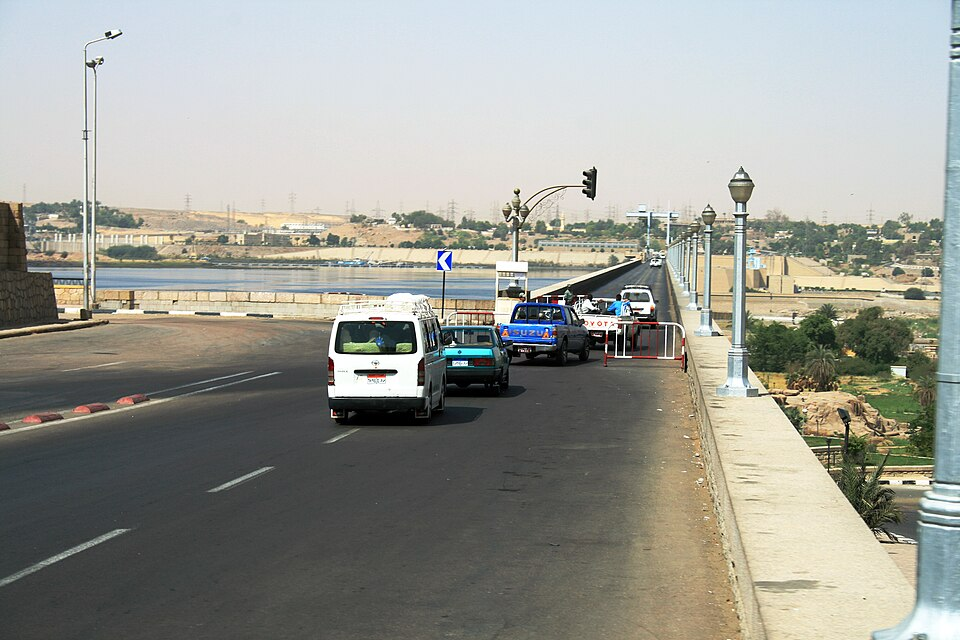
\includegraphics[height=0.17\textheight]{ch8_aswan_low_dam.jpg}\\[1mm]
\imgcap{Barajul Aswan Low (1902), pe Nil}
\imgcredit{https://commons.wikimedia.org/wiki/File:Aswan_Low_Dam_Egypt_1.jpg}{Foto: Karelj (2010); domeniu public; Wikimedia Commons}
\end{column}
\end{columns}
\end{frame}

\begin{frame}{Patru serii persistente}
\itemsize{\footnotesize}
\begin{center}
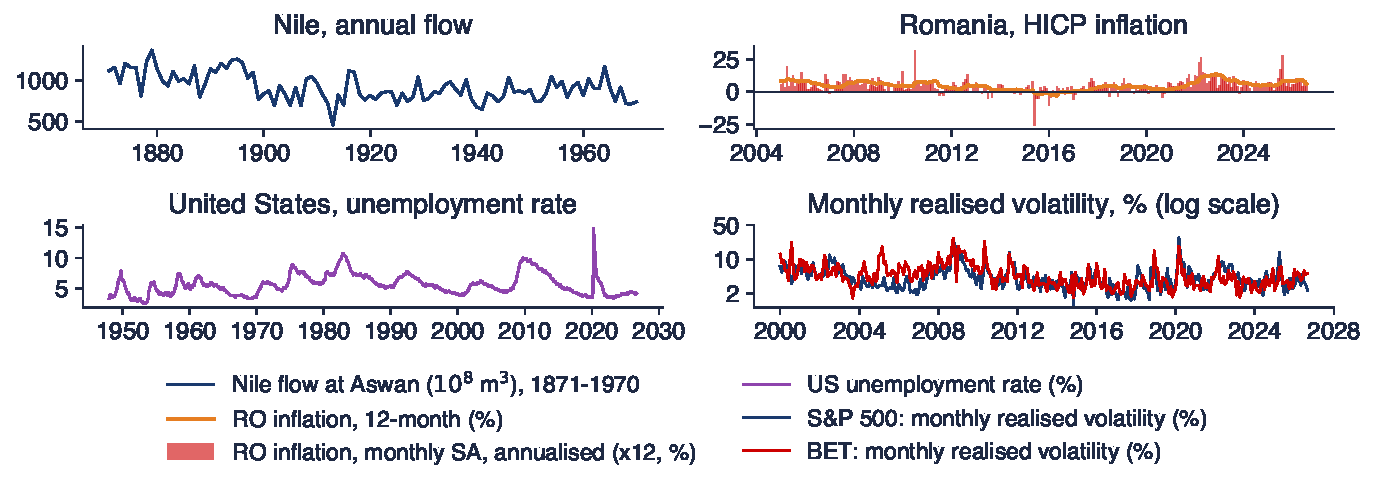
\includegraphics[width=0.97\textwidth,height=0.7\textheight,keepaspectratio]{tsa_ch8_memory_data.pdf}
\end{center}
\vspace{-0.25cm}
\begin{itemize}
    \item Debitul Nilului la Aswan, 1871--1970 (statsmodels); inflația IAPC din România, anuală și lunară, ajustată sezonier (SA) cu mediile lunare (Eurostat); rata șomajului din SUA (FRED UNRATE); volatilitatea realizată lunară a randamentelor zilnice S\&P 500 și BET (EODHD)
\end{itemize}
\quantlet{TSA\_ch8\_memory\_data}{\qlurl{TSA_ch8_memory_data}}
\end{frame}

\begin{frame}{Interpretarea celor patru serii}
\itemsize{\small}
\begin{itemize}
    \item Fiecare serie stă mult timp deasupra sau sub media ei
    \begin{itemize}
        \item Nilul: media 919 ($10^8$ m$^3$), perioade secetoase lungi după 1900; inflația anuală din România a atins 13{,}6\% în noiembrie 2022 și era 6{,}1\% în august 2026
    \end{itemize}
    \item Șomajul din SUA crește repede în recesiuni (maximum 14{,}8\% în aprilie 2020) și scade lent; ultima valoare 4{,}2\% (septembrie 2026)
    \begin{itemize}
        \item volatilitatea realizată: anii calmi alternează cu anii agitați; maxime 27\% (S\&P 500, martie 2020) și 27\% (BET, octombrie 2008)
    \end{itemize}
    \item Întrebarea capitolului: este aceasta o memorie care se stinge lent (lungă), o rădăcină aproape unitară sau o succesiune de regimuri?
\end{itemize}
\end{frame}

\begin{frame}{Memoria scurtă}
\itemsize{\small}
\begin{itemize}
    \item Reamintim (\tsachlink{https://danpele.github.io/Time-Series-Analysis/RO/Cursuri/capitol1_procese_stochastice_stationaritate.pdf}{Capitolul 1}): $\rho(k) = \gamma(k)/\gamma(0)$, autocorelația la decalajul $k$ a unei serii staționare
    \begin{itemize}
        \item \textbf{memorie scurtă}: autocorelațiile sînt absolut sumabile, $\sum_{k=0}^{\infty}|\rho(k)| < \infty$
    \end{itemize}
    \item Procesele ARMA staționare: $|\rho(k)| \le C r^k$, cu $0 < r < 1$: descreștere \textbf{exponențială}
    \begin{itemize}
        \item AR(1): $\rho(k) = \phi^k$; pentru $\phi = 0{,}9$, $\rho(50) = 0{,}005$: după 50 de perioade șocul este uitat
    \end{itemize}
    \item În domeniul frecvenței: densitatea spectrală $f(\lambda)$ este finită și pozitivă la frecvența $\lambda = 0$
    \begin{itemize}
        \item $f(0) = \frac{1}{2\pi}\sum_k \gamma(k)$: varianța pe termen lung este finită; varianța mediei de selecție scade ca $1/T$
    \end{itemize}
\end{itemize}
\end{frame}

\begin{frame}{Memoria lungă}
\itemsize{\small}
\begin{itemize}
    \item \textbf{Memorie lungă} (dependență pe termen lung): $\rho(k) \sim C\,k^{2d-1}$ cînd $k \to \infty$, cu $0 < d < 1/2$
    \begin{itemize}
        \item o descreștere \textbf{hiperbolică} (de tip putere): exponentul $2d - 1$ se află în $(-1, 0)$
        \item suma $\sum_k \rho(k)$ diverge: observațiile îndepărtate contează încă, luate împreună
    \end{itemize}
    \item În domeniul frecvenței: $f(\lambda) \sim G\,\lambda^{-2d}$ cînd $\lambda \to 0$: un \textbf{pol} la frecvența zero
    \begin{itemize}
        \item frecvențele joase (cicluri lente de toate lungimile) poartă cea mai mare parte a varianței
    \end{itemize}
    \item Consecință: $\Var(\bar{x}_T) \sim c\,T^{2d-1}$, mai lent decît $1/T$
    \begin{itemize}
        \item intervalele de încredere care presupun independența sînt prea înguste; parametrul de memorie $d$ măsoară cît de lent se estompează trecutul
    \end{itemize}
\end{itemize}
\end{frame}

\begin{frame}{ACF de selecție comparată cu un AR(1)}
\itemsize{\footnotesize}
\begin{center}
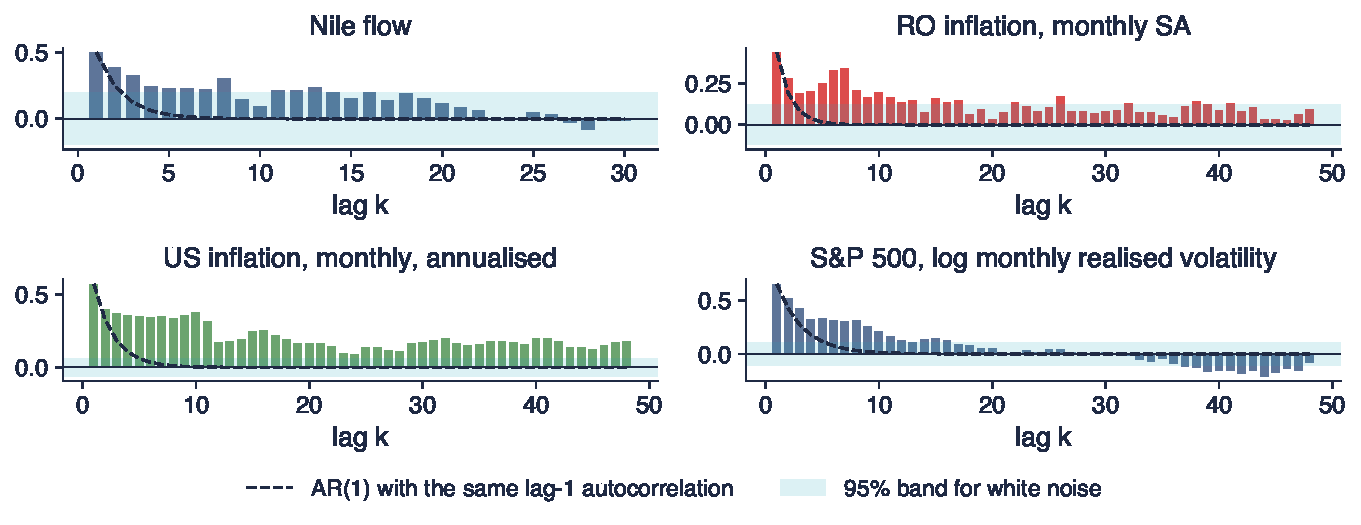
\includegraphics[width=0.97\textwidth,height=0.7\textheight,keepaspectratio]{tsa_ch8_memory_acf.pdf}
\end{center}
\vspace{-0.25cm}
\begin{itemize}
    \item Bare: ACF de selecție; linia punctată: $\hat\rho(1)^k$, ACF a unui AR(1) cu aceeași autocorelație de ordinul 1; zona colorată: $\pm 1{,}96/\sqrt{T}$
\end{itemize}
\quantlet{TSA\_ch8\_memory\_data}{\qlurl{TSA_ch8_memory_data}}
\end{frame}

\begin{frame}{Interpretarea ACF de selecție}
\itemsize{\small}
\begin{itemize}
    \item Nilul: $\hat\rho(1) = 0{,}50$; un AR(1) ar da $\rho(10) = 0{,}0009$, datele dau 0{,}09
    \begin{itemize}
        \item 11 dintre primele 30 autocorelații sînt deasupra benzii zgomotului alb
    \end{itemize}
    \item Inflația lunară din România: $\hat\rho(1) = 0{,}44$, $\hat\rho(10) = 0{,}20$; 22 din 48 de decalaje deasupra benzii
    \begin{itemize}
        \item inflația lunară din SUA: 48 din 48; logaritmul volatilității realizate S\&P 500: 15 din 48
    \end{itemize}
    \item O primă autocorelație moderată, urmată de o coadă lungă care scade lent, este semnătura memoriei lungi; un AR(1) nu o poate produce
\end{itemize}
\end{frame}

\begin{frame}{Descreștere hiperbolică și descreștere exponențială}
\itemsize{\footnotesize}
\begin{center}
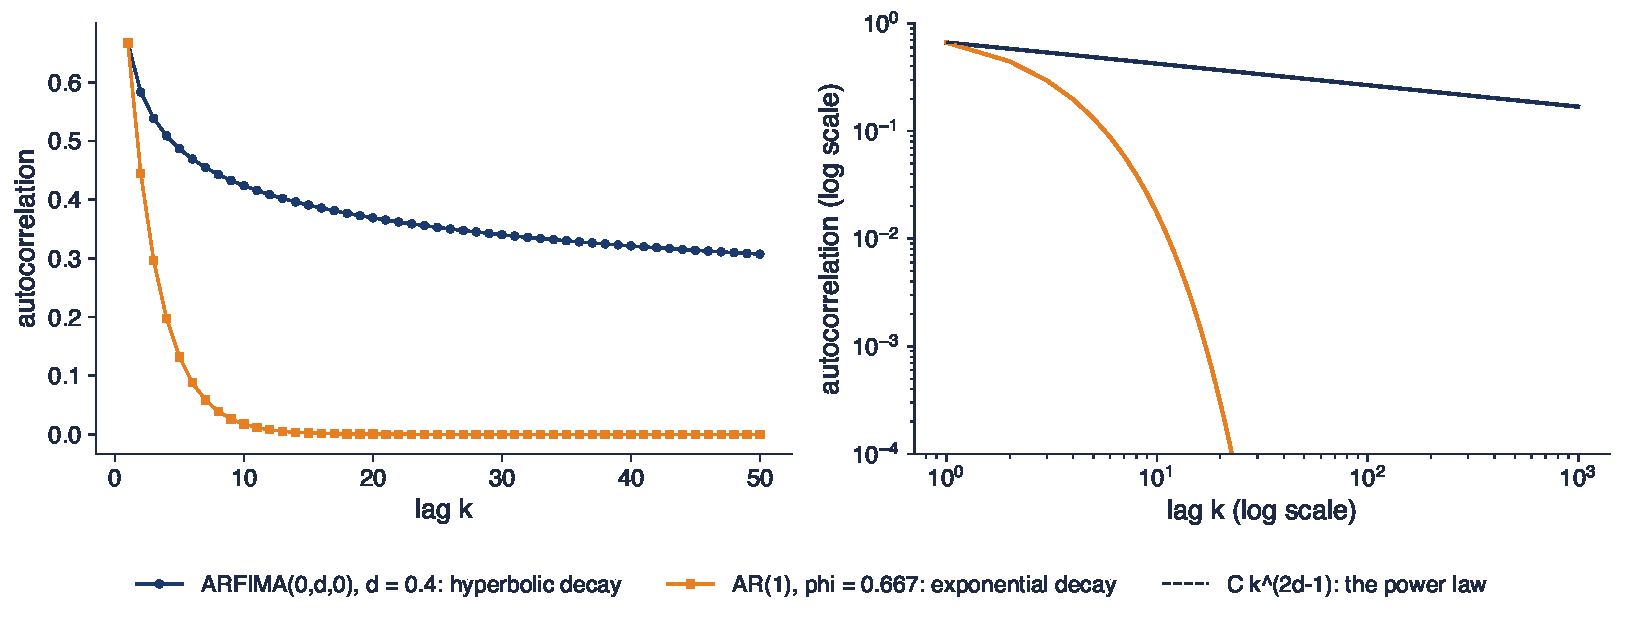
\includegraphics[width=0.97\textwidth,height=0.7\textheight,keepaspectratio]{tsa_ch8_decay.pdf}
\end{center}
\vspace{-0.25cm}
\begin{itemize}
    \item ACF teoretică a unui ARFIMA$(0,d,0)$ cu $d = 0{,}4$ (secțiunile următoare) și a unui AR(1) cu același $\rho(1) = d/(1-d) = 0{,}667$; dreapta: ambele pe axe log--log, cu legea de putere $C k^{2d-1}$
\end{itemize}
\quantlet{TSA\_ch8\_arfima\_processes}{\qlurl{TSA_ch8_arfima_processes}}
\end{frame}

\begin{frame}{Interpretarea celor două legi de descreștere}
\itemsize{\small}
\begin{itemize}
    \item Același început, cozi diferite: la decalajul 10, 0{,}424 față de 0{,}017; la decalajul 50, 0{,}307 față de $1{,}6 \cdot 10^{-9}$
    \begin{itemize}
        \item ACF cu memorie lungă este încă 0{,}169 la decalajul 1000
    \end{itemize}
    \item Pe axe log--log ACF hiperbolică devine o dreaptă de pantă $2d - 1 = -0{,}2$; ACF exponențială se curbează în jos
    \begin{itemize}
        \item panta unui grafic log--log este ideea din spatele tuturor estimatorilor din acest capitol
    \end{itemize}
    \item Sumele autocorelațiilor: AR(1) $\sum_{k\ge1}\phi^k = 2{,}0$; ARFIMA: 33{,}0 pînă la decalajul 100 și 210{,}4 pînă la decalajul 1000, în creștere
\end{itemize}
\end{frame}

\begin{frame}{Recapitulare: memorie scurtă și memorie lungă}
\itemsize{\small}
\begin{itemize}
    \item Memorie scurtă: ACF sumabilă, descreștere exponențială, spectru finit la zero (ARMA)
    \item Memorie lungă: $\rho(k) \sim Ck^{2d-1}$, ACF nesumabilă, pol spectral $f(\lambda) \sim G\lambda^{-2d}$
    \item Hurst și Nilul: amplitudinile cresc ca $n^H$, cu $H > 1/2$
    \item Inflația și volatilitatea au cozi lungi ale ACF, care scad lent
\end{itemize}
\end{frame}


%=============================================================================
\section{Diferențierea fracționară}
%=============================================================================

\begin{frame}{De la diferențe întregi la diferențe fracționare}
\itemsize{\small}
\begin{itemize}
    \item Operatorul de decalaj: $Lx_t = x_{t-1}$; prima diferență $(1-L)x_t = x_t - x_{t-1}$ (\tsachlink{https://danpele.github.io/Time-Series-Analysis/RO/Cursuri/capitol3_radacini_unitare_modele_arima.pdf}{Capitolul 3})
    \begin{itemize}
        \item $d = 0$: nivelul; $d = 1$: prima diferență; $d = 2$: $x_t - 2x_{t-1} + x_{t-2}$
    \end{itemize}
    \item \textbf{Diferența fracționară}, pentru orice $d$ real (seria binomială): $(1-L)^d = \sum_{k=0}^{\infty}\binom{d}{k}(-L)^k = \sum_{k=0}^{\infty}\pi_k L^k$
    \begin{itemize}
        \item $(1-L)^d = 1 - dL - \frac{d(1-d)}{2!}L^2 - \frac{d(1-d)(2-d)}{3!}L^3 - \dots$
        \item recurența: $\pi_0 = 1$, $\pi_k = \pi_{k-1}\,\dfrac{k - 1 - d}{k}$; pentru $k$ mare: $\pi_k \approx -\dfrac{d}{\Gamma(1-d)}\,k^{-1-d}$
    \end{itemize}
    \item O diferență fracționară folosește \textbf{toate} valorile trecute, cu ponderi care scad hiperbolic: elimină o parte din memorie, nu toată memoria
\end{itemize}
\end{frame}

\begin{frame}{Exemplu rezolvat: ponderile lui $(1-L)^{0{,}4}$}
\itemsize{\small}
\begin{itemize}
    \item Recurența $\pi_k = \pi_{k-1}(k - 1 - d)/k$ cu $d = 0{,}4$:
    \begin{itemize}
        \item $\pi_1 = 1 \cdot (0 - 0{,}4)/1 = -0{,}40$
        \item $\pi_2 = -0{,}40 \cdot (1 - 0{,}4)/2 = -0{,}12$
        \item $\pi_3 = -0{,}12 \cdot (2 - 0{,}4)/3 = -0{,}0640$; \quad $\pi_4 = -0{,}0640 \cdot 3{,}6/4 = -0{,}0416$; \quad $\pi_5 = -0{,}0300$
    \end{itemize}
    \item Deci $(1-L)^{0{,}4}x_t = x_t - 0{,}4x_{t-1} - 0{,}12x_{t-2} - 0{,}064x_{t-3} - 0{,}0416x_{t-4} - \dots$
    \begin{itemize}
        \item ponderile însumează $(1-1)^{0{,}4} = 0$ pe toate decalajele: un nivel constant este eliminat, ca la $d = 1$
    \end{itemize}
    \item Comparați cu $d = 1$: $\pi_1 = -1$, iar toate celelalte ponderi sînt 0; $d = 0{,}7$: $\pi_1 = -0{,}70$, $\pi_2 = -0{,}105$
\end{itemize}
\end{frame}

\begin{frame}{Diferențiere fracționară și integrare fracționară}
\itemsize{\footnotesize}
\begin{center}
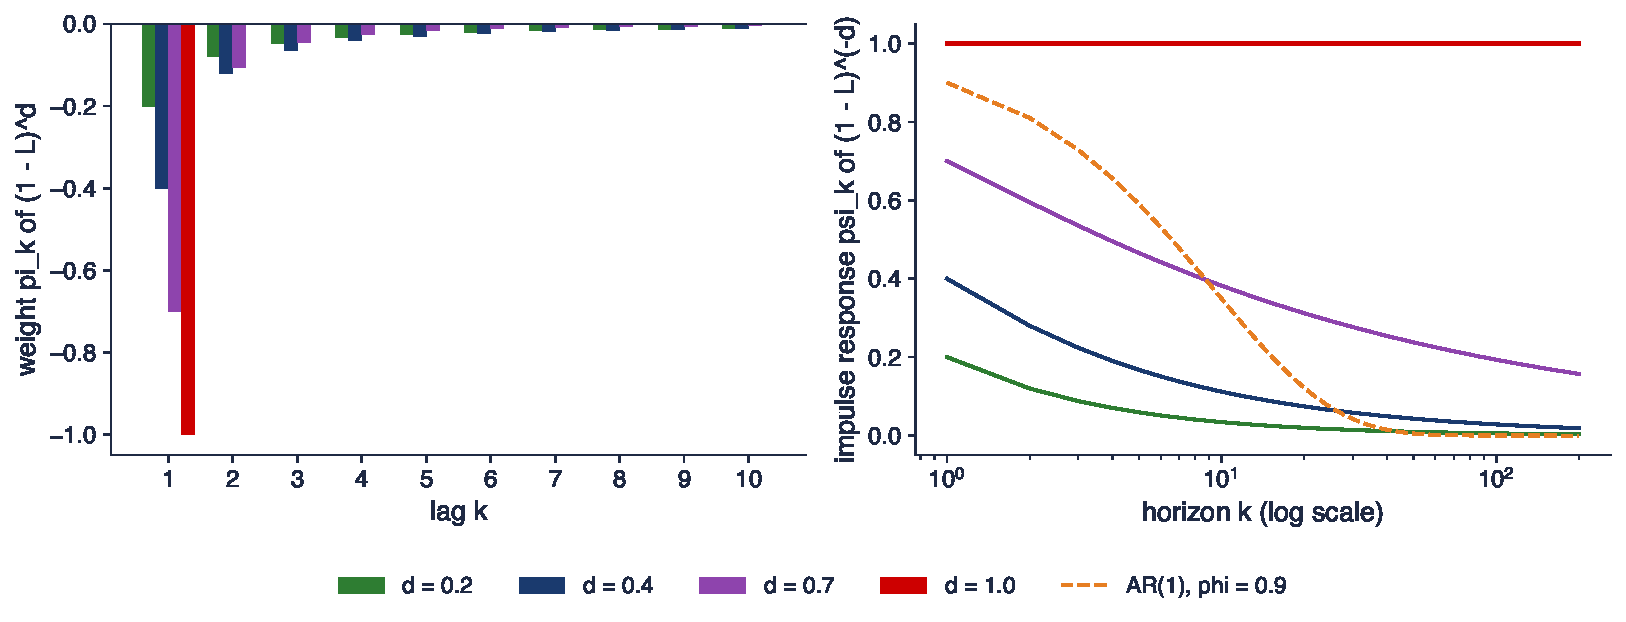
\includegraphics[width=0.97\textwidth,height=0.7\textheight,keepaspectratio]{tsa_ch8_weights.pdf}
\end{center}
\vspace{-0.25cm}
\begin{itemize}
    \item Stînga: ponderile $\pi_k$ ale lui $(1-L)^d$; dreapta: răspunsurile la impuls $\psi_k$ ale lui $(1-L)^{-d}$, adică efectul după $k$ perioade al unui șoc unitar asupra unei serii integrate fracționar, comparate cu un AR(1) cu $\phi = 0{,}9$
\end{itemize}
\quantlet{TSA\_ch8\_fractional\_differencing}{\qlurl{TSA_ch8_fractional_differencing}}
\end{frame}

\begin{frame}{Interpretarea ponderilor}
\itemsize{\small}
\begin{itemize}
    \item Integrarea fracționară: $x_t = (1-L)^{-d}\varepsilon_t = \sum_k\psi_k\varepsilon_{t-k}$, cu $\psi_k = \psi_{k-1}(k-1+d)/k \approx k^{d-1}/\Gamma(d)$
    \begin{itemize}
        \item după 100 de perioade un șoc are încă ponderea 0{,}028 ($d = 0{,}4$) și 0{,}193 ($d = 0{,}7$); AR(1) păstrează $2{,}7 \cdot 10^{-5}$
    \end{itemize}
    \item La început AR(1) își amintește mai mult (0{,}349 la decalajul 10, față de 0{,}112 pentru $d = 0{,}4$); apoi uită mult mai repede
    \begin{itemize}
        \item $d = 1$ (mers aleator): $\psi_k = 1$ mereu, șocul nu se stinge niciodată
    \end{itemize}
    \item Pentru $0 < d < 1$ răspunsurile tind spre zero: seria \textbf{revine la medie}, chiar și cînd este nestaționară ($d \ge 0{,}5$)
\end{itemize}
\end{frame}

\begin{frame}{Cîtă diferențiere îi trebuie unui preț?}
\itemsize{\footnotesize}
\begin{center}
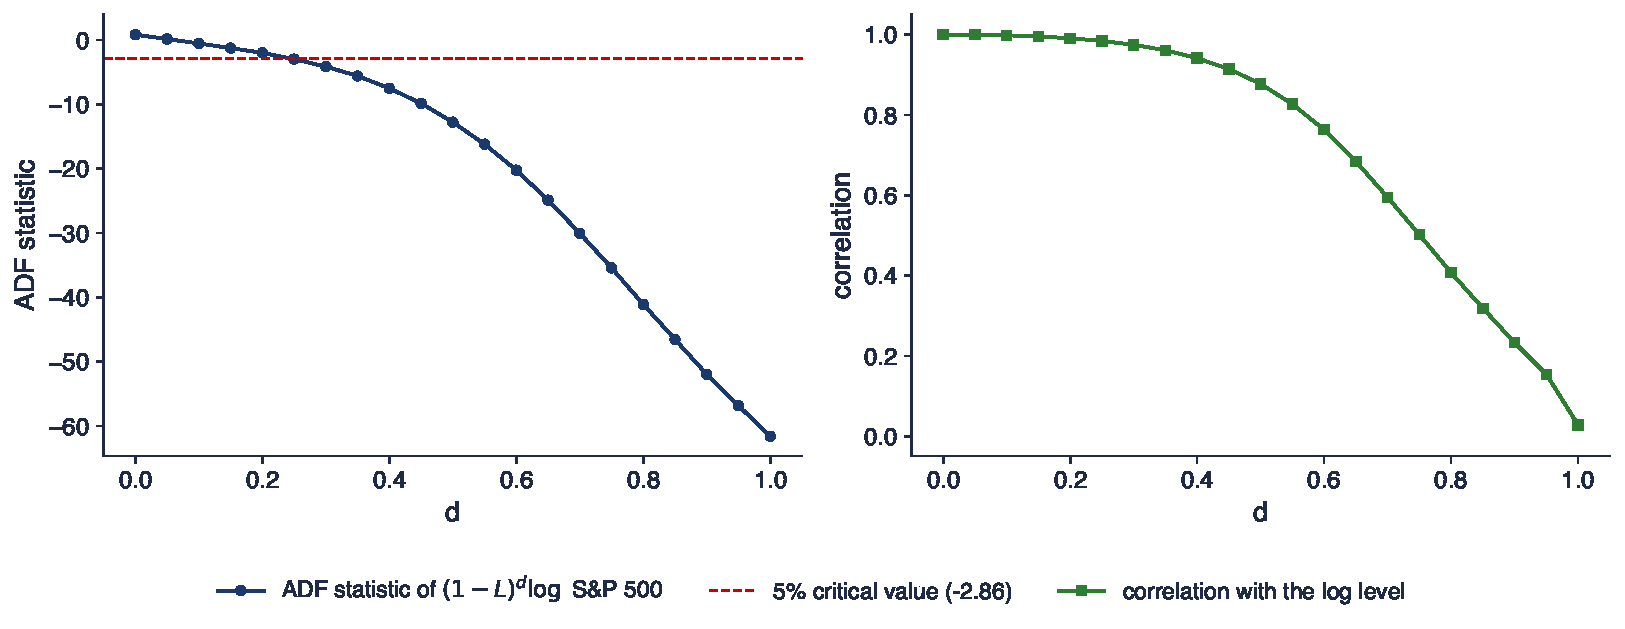
\includegraphics[width=0.97\textwidth,height=0.7\textheight,keepaspectratio]{tsa_ch8_ffd.pdf}
\end{center}
\vspace{-0.25cm}
\begin{itemize}
    \item Logaritmul S\&P 500, zilnic, 6\,715 de zile din 2000; $(1-L)^d$ cu fereastră fixă (ponderile sub $10^{-4}$ sînt eliminate), $d = 0;\ 0{,}05;\ \dots;\ 1$; stînga: statistica ADF (\tsachlink{https://danpele.github.io/Time-Series-Analysis/RO/Cursuri/capitol3_radacini_unitare_modele_arima.pdf}{Capitolul 3}); dreapta: corelația cu nivelul logaritmic
\end{itemize}
\quantlet{TSA\_ch8\_fractional\_differencing}{\qlurl{TSA_ch8_fractional_differencing}}
\end{frame}

\begin{frame}{Interpretarea diferențierii fracționare a unui preț}
\itemsize{\small}
\begin{itemize}
    \item Nivelul logaritmic ($d = 0$) are rădăcină unitară (ADF 0{,}84); randamentul ($d = 1$) este staționar (ADF -61{,}6), dar are corelația 0{,}03 cu nivelul
    \begin{itemize}
        \item prima diferență aruncă toată informația despre nivel
    \end{itemize}
    \item Statistica ADF trece de valoarea critică de 5\% (-2{,}86) deja la $d = 0{,}25$, unde corelația cu nivelul este încă 0{,}984
    \begin{itemize}
        \item fereastra fixă are atunci 445 de ponderi
    \end{itemize}
    \item O diferență fracționară poate face o serie staționară păstrîndu-i cea mai mare parte a memoriei: un instrument folosit pentru variabilele explicative din machine learning (\tsachlink{https://danpele.github.io/Time-Series-Analysis/RO/Cursuri/capitol9_invatare_automata_serii_timp.pdf}{Capitolul 9})
\end{itemize}
\end{frame}

\begin{frame}{Recapitulare: diferențierea fracționară}
\itemsize{\small}
\begin{itemize}
    \item $(1-L)^d = \sum_k\pi_k L^k$, $\pi_k = \pi_{k-1}(k-1-d)/k$: ponderi care scad hiperbolic
    \item $(1-L)^{-d}$: răspunsuri la impuls $\psi_k \approx k^{d-1}/\Gamma(d)$; revenire la medie pentru $d < 1$
    \item $d$ între 0 și 1 umple golul dintre niveluri și primele diferențe
\end{itemize}
\end{frame}


%=============================================================================
\section{Modelul ARFIMA$(p,d,q)$}
%=============================================================================

\begin{frame}{Modelul ARFIMA$(p,d,q)$}
\itemsize{\small}
\begin{itemize}
    \item \textbf{Definiție}: $\phi(L)(1-L)^d(x_t - \mu) = \theta(L)\varepsilon_t$, $\varepsilon_t$ zgomot alb cu varianța $\sigma^2$
    \begin{itemize}
        \item $\phi(L) = 1 - \phi_1L - \dots - \phi_pL^p$ și $\theta(L) = 1 + \theta_1L + \dots + \theta_qL^q$, cu rădăcinile în afara cercului unitate (\tsachlink{https://danpele.github.io/Time-Series-Analysis/RO/Cursuri/capitol2_modele_arma.pdf}{Capitolul 2})
        \item ARFIMA: autoregresiv, fracționar integrat, cu medie mobilă
    \end{itemize}
    \item Două părți cu două roluri
    \begin{itemize}
        \item $d$: memoria \textbf{pe termen lung}, coada hiperbolică a ACF
        \item $\phi$, $\theta$: dinamica \textbf{pe termen scurt}, primele cîteva autocorelații
    \end{itemize}
    \item Cazuri particulare: $d = 0$: ARMA$(p,q)$; $d = 1$: ARIMA$(p,1,q)$ (\tsachlink{https://danpele.github.io/Time-Series-Analysis/RO/Cursuri/capitol3_radacini_unitare_modele_arima.pdf}{Capitolul 3}); $d$ între ele: integrare fracționară, $x_t \sim I(d)$
\end{itemize}
\end{frame}

\begin{frame}{Granger, Joyeux și Hosking (1980--1981)}
\itemsize{\small}
\begin{columns}[T]
\begin{column}{0.38\textwidth}
\centering
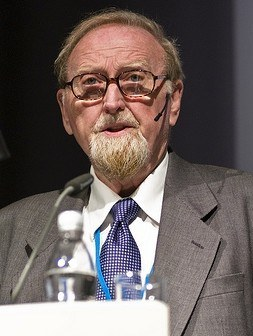
\includegraphics[height=0.48\textheight]{ch3_clive_granger_2008.jpg}\\[1mm]
\imgcap{Clive W. J. Granger (1934--2009), Premiul Nobel 2003}
\imgcredit{https://commons.wikimedia.org/wiki/File:Clive_Granger_by_Olaf_Storbeck_(3x4_cropped).jpg}{Foto: Olaf Storbeck (2008); CC BY-SA 2.0; Wikimedia Commons}
\end{column}
\begin{column}{0.6\textwidth}
\begin{itemize}
    \item \refGJ\ și \refHosking\ au introdus independent diferențierea fracționară
    \begin{itemize}
        \item Granger și Joyeux: agregarea multor serii AR(1) cu persistențe diferite produce memorie lungă
        \item Hosking: ACF, condițiile de staționaritate și de inversabilitate și familia ARFIMA$(p,d,q)$
    \end{itemize}
    \item Modelul lor leagă exponentul Hurst din hidrologie de modelele Box--Jenkins din econometrie
    \item Au urmat aplicații pentru inflație \refHW, producție, dobînzi și volatilitate \refDGE
\end{itemize}
\end{column}
\end{columns}
\end{frame}

\begin{frame}{Parametrul $d$: semnificația fiecărui interval}
\itemsize{\small}
\begin{center}
\footnotesize
\begin{tabular}{lll}
\toprule
\textbf{Intervalul lui $d$} & \textbf{Proprietăți} & \textbf{ACF / șocuri} \\
\midrule
$d \le -0{,}5$ & neinversabil (fără formă AR($\infty$)) & -- \\
$-0{,}5 < d < 0$ & staționar, inversabil, antipersistent & negativă, cu suma $-1/2$ \\
$d = 0$ & ARMA, memorie scurtă & descreștere exponențială \\
$0 < d < 0{,}5$ & staționar, memorie lungă & hiperbolică, nesumabilă \\
$0{,}5 \le d < 1$ & nestaționar, cu revenire la medie & șocurile se sting, lent \\
$d = 1$ & rădăcină unitară, ARIMA & șocurile sînt permanente \\
\bottomrule
\end{tabular}
\end{center}
\begin{itemize}
    \item Staționaritatea cere $d < 1/2$, inversabilitatea cere $d > -1/2$ (\refHosking); o serie nestaționară cu $d < 1{,}5$ se tratează diferențiind o dată: $(1-L)x_t \sim I(d-1)$
    \item Exponentul Hurst al incrementelor staționare: $H = d + 1/2$; $H > 1/2$ persistență, $H < 1/2$ antipersistență
\end{itemize}
\end{frame}

\begin{frame}{Autocorelațiile unui ARFIMA$(0,d,0)$}
\itemsize{\small}
\begin{itemize}
    \item Pentru $x_t = (1-L)^{-d}\varepsilon_t$, $-1/2 < d < 1/2$ (\refHosking):
    \begin{itemize}
        \item varianța $\gamma(0) = \sigma^2\,\dfrac{\Gamma(1-2d)}{\Gamma(1-d)^2}$
        \item autocorelațiile $\rho(k) = \dfrac{\Gamma(1-d)\,\Gamma(k+d)}{\Gamma(d)\,\Gamma(k+1-d)}$, calculate cu $\rho(k) = \rho(k-1)\,\dfrac{k-1+d}{k-d}$
    \end{itemize}
    \item Primele decalaje: $\rho(1) = \dfrac{d}{1-d}$, \quad $\rho(2) = \dfrac{d(1+d)}{(1-d)(2-d)}$
    \begin{itemize}
        \item $k$ mare: $\rho(k) \approx \dfrac{\Gamma(1-d)}{\Gamma(d)}\,k^{2d-1}$, legea de putere din secțiunea 1, cu $C = \Gamma(1-d)/\Gamma(d)$
    \end{itemize}
    \item Densitatea spectrală: $f(\lambda) = \dfrac{\sigma^2}{2\pi}\,|1 - e^{-i\lambda}|^{-2d} = \dfrac{\sigma^2}{2\pi}\,\bigl(2\sin(\lambda/2)\bigr)^{-2d} \approx \dfrac{\sigma^2}{2\pi}\lambda^{-2d}$ în apropierea lui 0
\end{itemize}
\end{frame}

\begin{frame}{Exemplu rezolvat: ARFIMA$(0;\ 0{,}3;\ 0)$}
\itemsize{\small}
\begin{itemize}
    \item $\rho(1) = 0{,}3/0{,}7 = 0{,}429$; \quad $\rho(2) = 0{,}429 \cdot 1{,}3/1{,}7 = 0{,}328$; \quad $\rho(3) = 0{,}328 \cdot 2{,}3/2{,}7 = 0{,}279$
    \begin{itemize}
        \item continuînd recurența: $\rho(5) = 0{,}228$, $\rho(10) = 0{,}173$
    \end{itemize}
    \item Varianța pentru $\sigma^2 = 1$: $\Gamma(0{,}4)/\Gamma(0{,}7)^2 = 1{,}316$, mai mare decît varianța șocurilor
    \begin{itemize}
        \item memoria acumulează șocurile trecute
    \end{itemize}
    \item Un AR(1) cu același $\rho(1) = 0{,}429$ are $\rho(10) = 0{,}429^{10} = 0{,}0002$: cu trei ordine de mărime sub 0{,}173
    \item $H = d + 0{,}5 = 0{,}8$: o serie persistentă
\end{itemize}
\end{frame}

\begin{frame}{ARFIMA$(0,d,0)$ cu $d = 0{,}4$ și $d = -0{,}4$}
\itemsize{\footnotesize}
\begin{center}
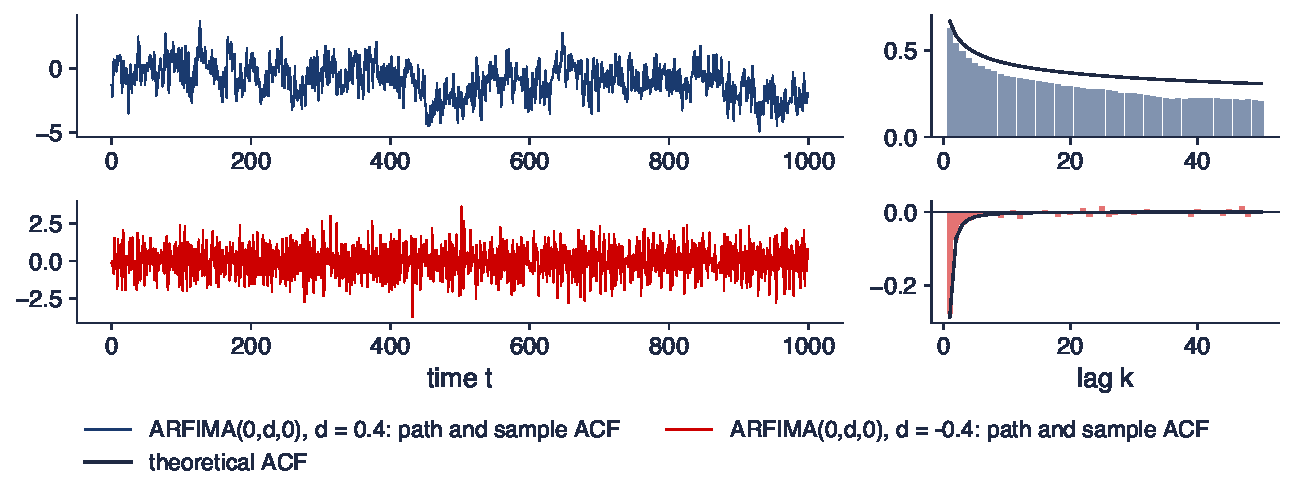
\includegraphics[width=0.97\textwidth,height=0.7\textheight,keepaspectratio]{tsa_ch8_arfima_paths.pdf}
\end{center}
\vspace{-0.25cm}
\begin{itemize}
    \item Traiectorii simulate (1000 de observații, simulare exactă prin scufundare circulantă) cu $\varepsilon_t \sim N(0, 1)$; dreapta: ACF de selecție pentru 20\,000 de observații și ACF teoretică
\end{itemize}
\quantlet{TSA\_ch8\_arfima\_processes}{\qlurl{TSA_ch8_arfima_processes}}
\end{frame}

\begin{frame}{Interpretarea celor două traiectorii ARFIMA}
\itemsize{\small}
\begin{itemize}
    \item $d = 0{,}4$: excursii lungi deasupra și sub zero; $\rho(1) = 0{,}667$, $\rho(10) = 0{,}424$, $\rho(50) = 0{,}307$; varianța 2{,}07
    \begin{itemize}
        \item traiectoria pare să aibă trenduri, deși media este constantă: un motiv pentru care memoria lungă este confundată cu nestaționaritatea
    \end{itemize}
    \item $d = -0{,}4$: zig-zag rapid; $\rho(1) = -0{,}286$, $\rho(2) = -0{,}071$; varianța 1{,}18
    \begin{itemize}
        \item antipersistență: o creștere tinde să fie urmată de o scădere; tipică seriilor diferențiate excesiv, de exemplu diferența unei serii cu $d = 0{,}6$
    \end{itemize}
\end{itemize}
\end{frame}

\begin{frame}{Mandelbrot: mișcarea browniană fracționară și $H$}
\itemsize{\small}
\begin{columns}[T]
\begin{column}{0.38\textwidth}
\centering
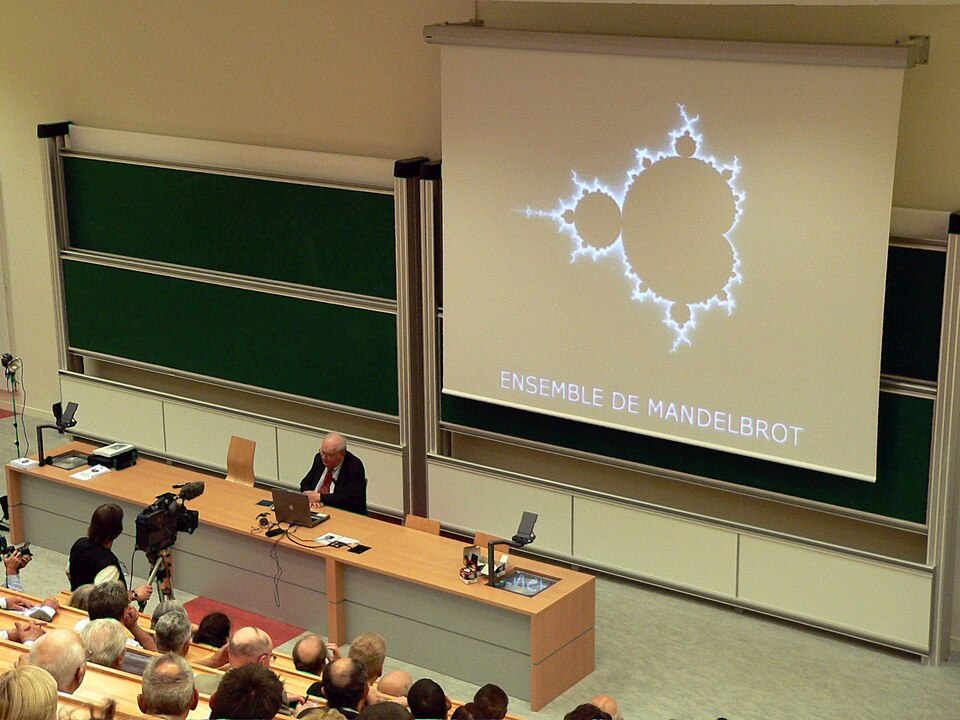
\includegraphics[height=0.42\textheight]{ch8_mandelbrot_2006.jpg}\\[1mm]
\imgcap{Benoît Mandelbrot (1924--2010)}
\imgcredit{https://commons.wikimedia.org/wiki/File:Mandelbrot_p1130876.jpg}{Foto: David Monniaux (2006); CC BY-SA 3.0; Wikimedia Commons}
\end{column}
\begin{column}{0.6\textwidth}
\begin{itemize}
    \item \textbf{Mișcarea browniană fracționară} $B_H(t)$, $0 < H < 1$ \refMVN: gaussiană, $B_H(0) = 0$, $\Var(B_H(t)) = t^{2H}$
    \begin{itemize}
        \item autosimilară: $B_H(ct)$ are aceeași distribuție ca $c^H B_H(t)$; $H = 1/2$: mișcarea browniană
    \end{itemize}
    \item Incrementele ei, \textbf{zgomotul gaussian fracționar} (fGn), sînt staționare, cu $\rho(k) = \tfrac12(|k+1|^{2H} - 2|k|^{2H} + |k-1|^{2H})$
    \begin{itemize}
        \item $\rho(k) \approx H(2H-1)k^{2H-2}$: aceeași coadă ca ARFIMA cu $d = H - 1/2$
    \end{itemize}
    \item Mandelbrot a adus rezultatul lui Hurst în statistică: fGn este varianta în timp continuu a unui ARFIMA$(0,d,0)$
\end{itemize}
\end{column}
\end{columns}
\end{frame}

\begin{frame}{Mișcarea browniană fracționară pentru trei exponenți Hurst}
\itemsize{\footnotesize}
\begin{center}
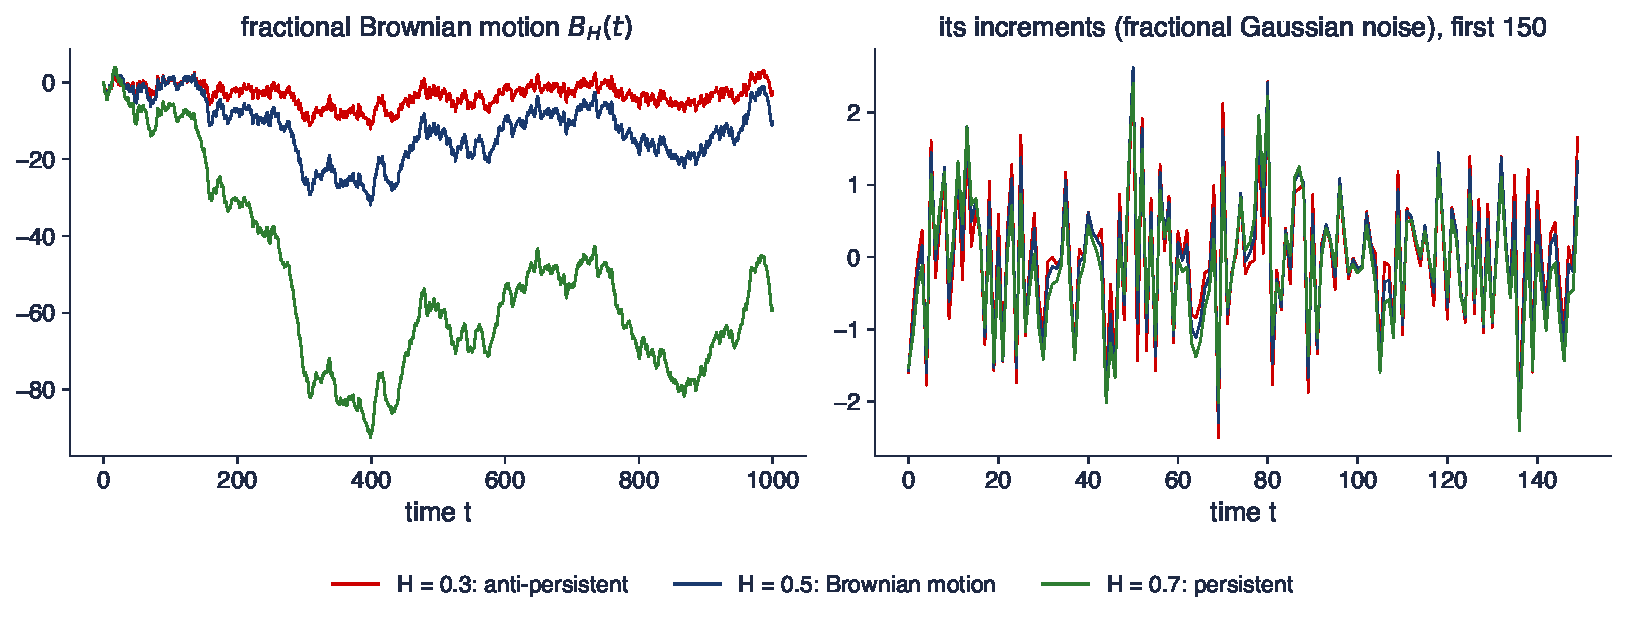
\includegraphics[width=0.97\textwidth,height=0.7\textheight,keepaspectratio]{tsa_ch8_fbm.pdf}
\end{center}
\vspace{-0.25cm}
\begin{itemize}
    \item Aceleași numere aleatoare pentru $H = 0{,}3$, $0{,}5$ și $0{,}7$ (scufundare circulantă); dreapta: primele 150 de incremente
\end{itemize}
\quantlet{TSA\_ch8\_arfima\_processes}{\qlurl{TSA_ch8_arfima_processes}}
\end{frame}

\begin{frame}{Interpretarea traiectoriilor fBm}
\itemsize{\small}
\begin{itemize}
    \item $H = 0{,}7$: traiectorie netedă, cu aparență de trend; autocorelația de ordinul 1 a incrementelor $2^{2H-1} - 1 = 0{,}32$ (în eșantion 0{,}32)
    \begin{itemize}
        \item $H = 0{,}3$: traiectorie aspră, care se întoarce mereu; $\rho(1) = -0{,}24$ (în eșantion -0{,}23)
    \end{itemize}
    \item Amplitudinea traiectoriei crește ca $t^H$: mărimea pe care a măsurat-o Hurst pe Nil
    \item În modelarea seriilor de timp preferăm ARFIMA: adaugă partea ARMA pe termen scurt, care lipsește din fGn
\end{itemize}
\end{frame}

\begin{frame}{Recapitulare: modelul ARFIMA}
\itemsize{\small}
\begin{itemize}
    \item $\phi(L)(1-L)^d(x_t - \mu) = \theta(L)\varepsilon_t$: $d$ pentru termenul lung, ARMA pentru termenul scurt
    \item Staționar pentru $d < 1/2$, inversabil pentru $d > -1/2$; cu revenire la medie pentru $d < 1$
    \item ARFIMA$(0,d,0)$: $\rho(1) = d/(1-d)$, $\rho(k) \sim Ck^{2d-1}$; $H = d + 1/2$
    \item fBm și fGn: aceeași memorie lungă, în forma în timp continuu a lui Mandelbrot
\end{itemize}
\end{frame}


%=============================================================================
\section{Estimarea lui $d$}
%=============================================================================

\begin{frame}{Cinci estimatori}
\itemsize{\small}
\begin{center}
\scriptsize
\begin{tabular}{>{\raggedright\arraybackslash}p{2.3cm}>{\raggedright\arraybackslash}p{3.1cm}>{\raggedright\arraybackslash}p{3.6cm}>{\raggedright\arraybackslash}p{1.9cm}}
\toprule
\textbf{Estimatorul} & \textbf{Folosește} & \textbf{Estimarea} & \textbf{Tipul} \\
\midrule
R/S \refHurst{} & amplitudinea sumelor parțiale pe blocuri & panta lui $\log(R/S)_n$ față de $\log n$ = $H$ & euristic \\
DFA \refPeng{} & fluctuațiile fără tendință ale profilului & panta lui $\log F(n)$ față de $\log n$ = $H$ & euristic \\
GPH \refGPH{} & primele $m$ valori ale periodogramei & panta OLS a unei regresii pe log-periodogramă & semiparametric \\
Whittle local \refRob{} & primele $m$ valori ale periodogramei & maximizează o verosimilitate gaussiană locală & semiparametric \\
ML exactă, Whittle \refSowell, \refFT{} & toată seria & $d$, $\phi$, $\theta$, $\sigma^2$ împreună & parametric \\
\bottomrule
\end{tabular}
\end{center}
\begin{itemize}
    \item Semiparametric: se modelează doar comportamentul din apropierea frecvenței zero, partea pe termen scurt rămîne liberă; parametric: întregul model ARFIMA trebuie să fie corect
    \item ML: verosimilitate maximă; OLS: metoda celor mai mici pătrate; $d = H - 1/2$ face trecerea între cele două scale
\end{itemize}
\end{frame}

\begin{frame}{Statistica R/S, pas cu pas}
\itemsize{\footnotesize}
\begin{itemize}
    \item Blocul $x_1, \dots, x_n$: media $\bar x$, abaterile cumulate $Y_k = \sum_{i\le k}(x_i - \bar x)$
    \begin{itemize}
        \item amplitudinea $R = \max_k Y_k - \min_k Y_k$, abaterea standard $S$; amplitudinea rescalată $R/S$
    \end{itemize}
    \item Exemplu: $x = (0{,}5;\ -0{,}3;\ 0{,}8;\ -0{,}2;\ 0{,}6;\ -0{,}1;\ 0{,}4;\ -0{,}7)$, $\bar x = 0{,}125$
    \begin{itemize}
        \item $Y_k$: 0,375; $-$0,050; 0,625; 0,300; 0,775; 0,550; 0,825; 0; $R = 0{,}825 - (-0{,}050) = 0{,}875$
        \item $S = 0{,}489$, deci $R/S = 1{,}79$
    \end{itemize}
    \item \textbf{Exponentul Hurst}: media $(R/S)_n$ pe blocuri de mărime $n$; $E(R/S)_n \approx c\,n^H$, deci $H$ este panta lui $\log(R/S)_n$ față de $\log n$
    \begin{itemize}
        \item capcane: deplasat în sus pe blocuri mici \refMW; și memoria scurtă îl crește; \refLo\ corectează $S$ cu autocovarianțe (R/S modificat)
        \item \textbf{DFA} \refPeng: ajustăm o dreaptă profilului $Y_k$ în fiecare bloc; $F(n)$, abaterea medie pătratică (RMS), crește ca $n^H$
    \end{itemize}
\end{itemize}
\end{frame}

\begin{frame}{R/S și DFA pentru trei serii}
\itemsize{\footnotesize}
\begin{center}
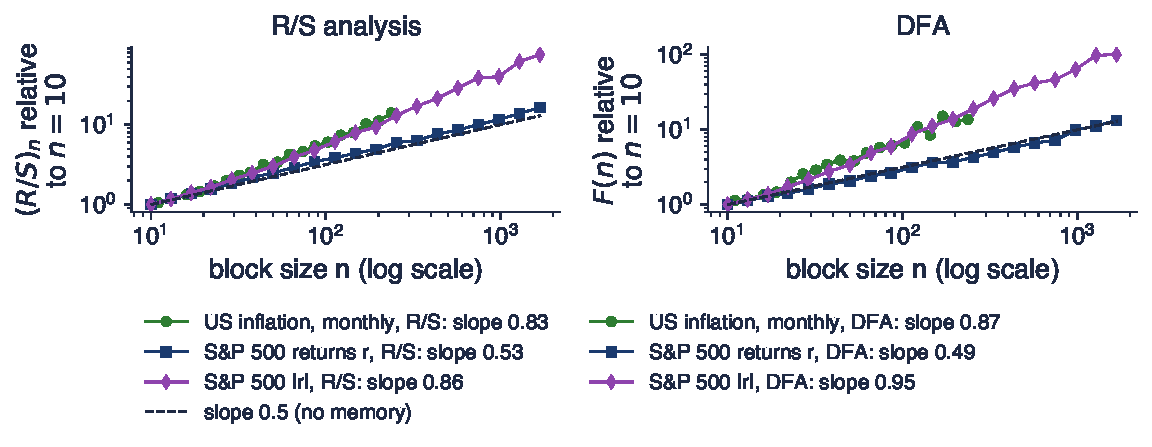
\includegraphics[width=0.97\textwidth,height=0.7\textheight,keepaspectratio]{tsa_ch8_rs_dfa.pdf}
\end{center}
\vspace{-0.25cm}
\begin{itemize}
    \item Inflația lunară din SUA (FRED CPIAUCSL, 1947--2026), randamentele zilnice S\&P 500 $r_t$ și randamentele absolute $|r_t|$ (2000--2026); ambele axe logaritmice, curbele normalizate la 1 pentru $n = 10$
\end{itemize}
\quantlet{TSA\_ch8\_hurst\_rs\_dfa}{\qlurl{TSA_ch8_hurst_rs_dfa}}
\end{frame}

\begin{frame}{Interpretarea pantelor R/S și DFA}
\itemsize{\small}
\begin{itemize}
    \item Randamentele S\&P 500: pantele 0{,}53 (R/S) și 0{,}49 (DFA), apropiate de 0,5: fără memorie în randamente
    \begin{itemize}
        \item eficiența slabă din \tsachlink{https://danpele.github.io/Time-Series-Analysis/RO/Cursuri/capitol3_radacini_unitare_modele_arima.pdf}{Capitolul 3} este valabilă pentru randamente
    \end{itemize}
    \item Randamentele absolute: 0{,}86 și 0{,}95; inflația din SUA: 0{,}83 și 0{,}87
    \begin{itemize}
        \item ambele mult peste 0,5: persistente; o pantă DFA apropiată de 1 sugerează un $d$ apropiat de 0,5, limita staționarității
    \end{itemize}
    \item Acestea sînt instrumente grafice: nu dau o eroare standard și reacționează la memoria scurtă și la trenduri; estimatorii următori sînt construiți pentru inferență
\end{itemize}
\end{frame}

\begin{frame}{Periodograma și estimatorul GPH}
\itemsize{\small}
\begin{itemize}
    \item \textbf{Periodograma} la frecvențele Fourier $\lambda_j = 2\pi j/T$: $I(\lambda_j) = \frac{1}{2\pi T}\bigl|\sum_t (x_t - \bar x)e^{-i\lambda_j t}\bigr|^2$
    \begin{itemize}
        \item o estimare zgomotoasă a densității spectrale $f(\lambda_j)$; $\lambda_j$ apropiat de 0 = cicluri lente, de perioadă $T/j$
    \end{itemize}
    \item În apropierea lui zero, $f(\lambda) \approx G\,(4\sin^2(\lambda/2))^{-d}$; logaritmînd:
    \begin{itemize}
        \item \textbf{Regresia GPH} \refGPH: $\log I(\lambda_j) = c + d\,\bigl[-\log(4\sin^2(\lambda_j/2))\bigr] + u_j$, $j = 1, \dots, m$
        \item $\hat d$ = panta OLS; eroarea standard $\pi/\sqrt{24m}$
    \end{itemize}
    \item \textbf{Lățimea de bandă} $m$: cîte frecvențe joase folosim; aici $m = \lfloor T^{0{,}65}\rfloor$
    \begin{itemize}
        \item $m$ mic: puțină deplasare din partea pe termen scurt, varianță mare; $m$ mare: varianță mică, dar memoria scurtă se strecoară în $\hat d$
    \end{itemize}
\end{itemize}
\end{frame}

\begin{frame}{Regresii GPH: Nilul și inflația din România}
\itemsize{\footnotesize}
\begin{center}
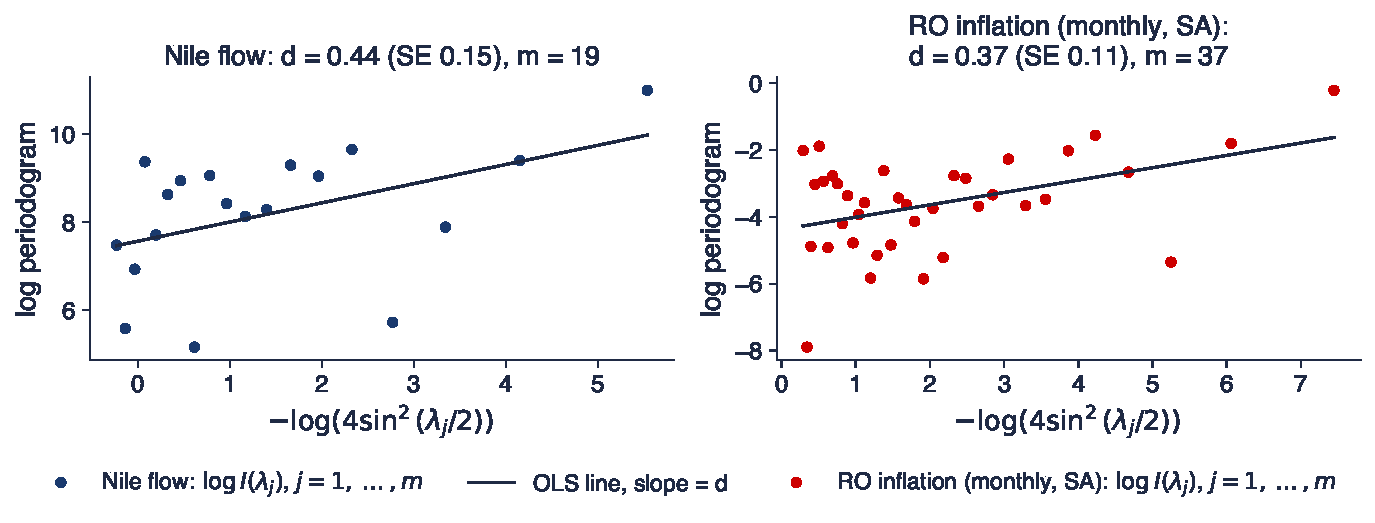
\includegraphics[width=0.97\textwidth,height=0.7\textheight,keepaspectratio]{tsa_ch8_gph.pdf}
\end{center}
\vspace{-0.25cm}
\begin{itemize}
    \item Puncte: logaritmul periodogramei la cele mai joase $m$ frecvențe Fourier; linia: ajustarea OLS. Nilul: $T = 100$ de ani; inflația lunară din România (SA): $T = 260$ de luni, ultima august 2026
\end{itemize}
\quantlet{TSA\_ch8\_estimation}{\qlurl{TSA_ch8_estimation}}
\end{frame}

\begin{frame}{Interpretarea regresiilor GPH}
\itemsize{\small}
\begin{itemize}
    \item Nilul: $\hat d = 0{,}44$ (SE 0{,}15), $m = 19$ frecvențe, adică cicluri mai lungi de 5{,}3 ani
    \begin{itemize}
        \item Whittle local (slide-ul următor): 0{,}40 (SE 0{,}11); ambele semnificativ peste 0, în intervalul staționar
    \end{itemize}
    \item Inflația din România: $\hat d = 0{,}37$ (SE 0{,}11); Whittle local 0{,}31 (SE 0{,}08)
    \begin{itemize}
        \item cicluri mai lungi de 7{,}0 luni: un șoc al inflației lunare se stinge în ani, nu în luni
    \end{itemize}
    \item Norul de puncte este larg: fiecare valoare a periodogramei este aproximativ o variabilă exponențială în jurul lui $f(\lambda_j)$; panta are nevoie de multe puncte
\end{itemize}
\end{frame}

\begin{frame}{Estimatorul Whittle local}
\itemsize{\small}
\begin{itemize}
    \item \refRob: presupunem $f(\lambda) \approx G\lambda^{-2d}$ pentru $\lambda_1, \dots, \lambda_m$ și maximizăm verosimilitatea gaussiană (Whittle) a acestor valori
    \begin{itemize}
        \item după eliminarea lui $G$: $\hat d = \arg\min_d\ \log\Bigl(\frac1m\sum_{j=1}^m \lambda_j^{2d}I(\lambda_j)\Bigr) - \frac{2d}{m}\sum_{j=1}^m\log\lambda_j$
    \end{itemize}
    \item Eroarea standard $1/(2\sqrt m)$, mai mică decît la GPH ($\pi/\sqrt{24m} \approx 0{,}64/\sqrt m$)
    \begin{itemize}
        \item valabil și pentru serii nestaționare cu $d$ pînă la aproximativ 1 \refVelasco
    \end{itemize}
    \item Atît GPH, cît și Whittle local depind de $m$: raportați întotdeauna $\hat d$ pentru mai multe lățimi de bandă
\end{itemize}
\end{frame}

\begin{frame}{Sensibilitatea la lățimea de bandă}
\itemsize{\footnotesize}
\begin{center}
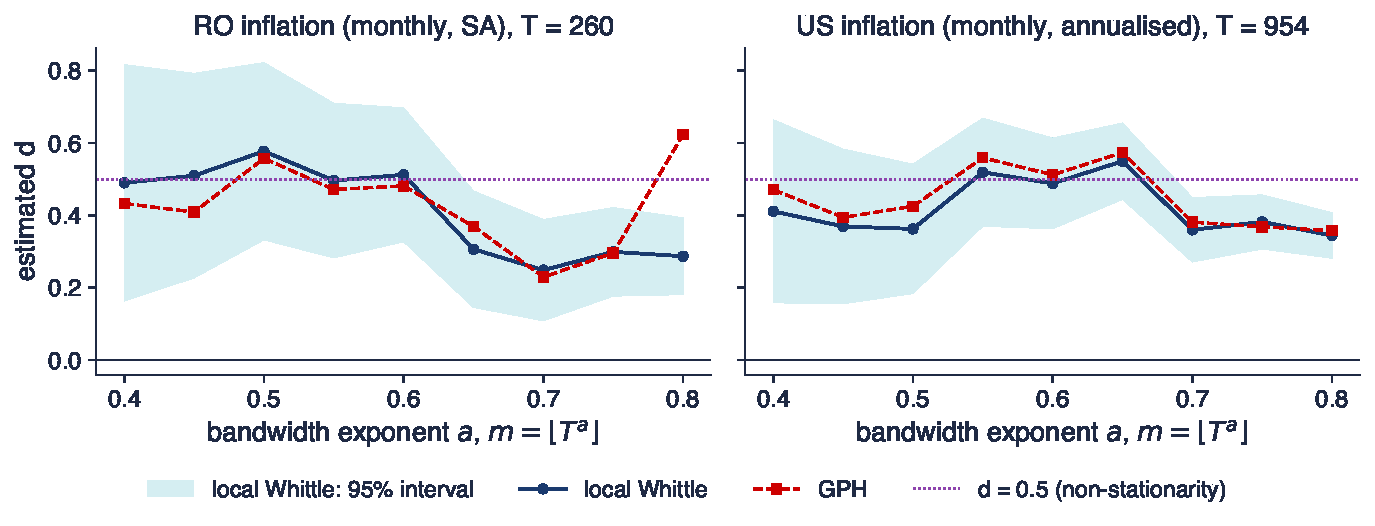
\includegraphics[width=0.97\textwidth,height=0.7\textheight,keepaspectratio]{tsa_ch8_bandwidth.pdf}
\end{center}
\vspace{-0.25cm}
\begin{itemize}
    \item $\hat d$ pentru $m = \lfloor T^a\rfloor$, $a = 0{,}40;\ \dots;\ 0{,}80$; zona colorată: intervalul de 95\% al estimatorului Whittle local. Inflația lunară din România ($T = 260$, $m$ de la 9 la 85) și inflația lunară din SUA ($T = 954$)
\end{itemize}
\quantlet{TSA\_ch8\_estimation}{\qlurl{TSA_ch8_estimation}}
\end{frame}

\begin{frame}{Interpretarea graficului lățimii de bandă}
\itemsize{\small}
\begin{itemize}
    \item România: Whittle local între 0{,}25 și 0{,}58, GPH între 0{,}23 și 0{,}62
    \begin{itemize}
        \item cu puține frecvențe estimarea este aproape de 0,5; cu mai multe scade spre 0,3: răspunsul depinde de alegerea lui $m$
    \end{itemize}
    \item Statele Unite: Whittle local între 0{,}34 și 0{,}55, mereu mult peste 0
    \begin{itemize}
        \item eșantionul lung (1947--2026) dă intervale înguste; un $d$ apropiat de 0,5 sugerează schimbări de regim (secțiunea 7)
    \end{itemize}
    \item Concluzie: inflația are memorie lungă în ambele țări; un singur număr pentru $d$ ascunde o incertitudine de aproximativ $\pm 0{,}15$
\end{itemize}
\end{frame}

\begin{frame}{Verosimilitatea maximă pentru ARFIMA$(p,d,q)$}
\itemsize{\footnotesize}
\begin{itemize}
    \item \textbf{ML exactă} \refSowell: pentru $x = (x_1, \dots, x_T)'$ gaussian, cu matricea de covarianță $\Gamma(\vartheta)$, $\vartheta = (d, \phi, \theta, \sigma^2)$:
    \begin{itemize}
        \item $\ell(\vartheta) = -\frac{T}{2}\log 2\pi - \frac12\log\det\Gamma(\vartheta) - \frac12 (x - \mu)'\Gamma(\vartheta)^{-1}(x - \mu)$
        \item $\Gamma$ provine din autocovarianțele ARFIMA; recurența Durbin--Levinson calculează $\ell$ în $O(T^2)$ operații
    \end{itemize}
    \item \textbf{Whittle} (ML aproximativă) \refFT: înlocuim verosimilitatea cu $-\frac12\sum_j\bigl[\log f(\lambda_j;\vartheta) + I(\lambda_j)/f(\lambda_j;\vartheta)\bigr]$ pe toate frecvențele Fourier
    \begin{itemize}
        \item rapidă ($O(T\log T)$ cu FFT, transformata Fourier rapidă), apropiată de ML exactă în eșantioane mari
    \end{itemize}
    \item Estimatorii parametrici sînt eficienți (SE în jur de $\sqrt{6}/(\pi\sqrt T)$ pentru ARFIMA$(0,d,0)$) doar dacă ordinele ARMA sînt corecte; alegem $p$, $q$ după AIC/BIC
\end{itemize}
\end{frame}

\begin{frame}{Monte Carlo: cinci estimatori ai lui $d$}
\itemsize{\footnotesize}
\begin{center}
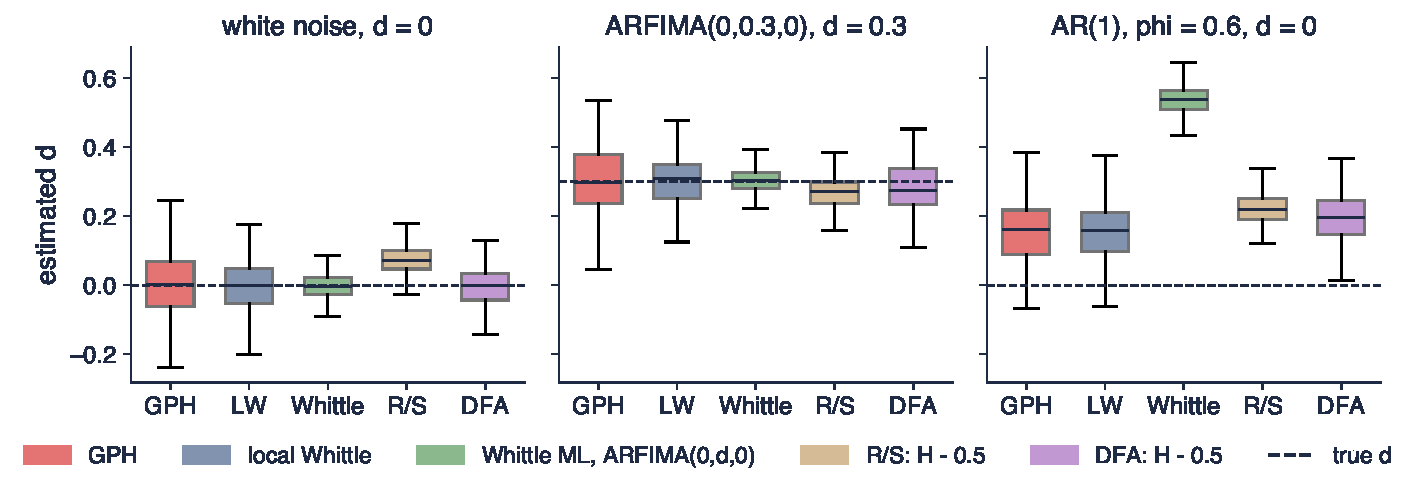
\includegraphics[width=0.97\textwidth,height=0.7\textheight,keepaspectratio]{tsa_ch8_mc.pdf}
\end{center}
\vspace{-0.25cm}
\begin{itemize}
    \item 300 de eșantioane de $T = 500$ pentru fiecare variantă; GPH și Whittle local cu $m = \lfloor T^{0{,}65}\rfloor$; ML Whittle pentru ARFIMA$(0,d,0)$; R/S și DFA convertite cu $d = H - 1/2$
\end{itemize}
\quantlet{TSA\_ch8\_monte\_carlo}{\qlurl{TSA_ch8_monte_carlo}}
\end{frame}

\begin{frame}{Interpretarea simulării Monte Carlo}
\itemsize{\small}
\begin{itemize}
    \item Model corect: ML Whittle este cel mai precis (abaterea standard 0{,}04, față de 0{,}08 pentru Whittle local și 0{,}10 pentru GPH la $d = 0{,}3$)
    \begin{itemize}
        \item R/S este deplasat în sus pentru zgomot alb (media 0{,}07) \refMW
    \end{itemize}
    \item AR(1) cu $\phi = 0{,}6$, fără memorie lungă: ARFIMA$(0,d,0)$ prin Whittle dă 0{,}54, GPH 0{,}15, Whittle local 0{,}15
    \begin{itemize}
        \item un model parametric greșit specificat transformă memoria scurtă în „memorie lungă”; estimatorii semiparametrici sînt mai puțin afectați, dar nu sînt imuni
    \end{itemize}
    \item În practică: estimați întotdeauna și ARFIMA$(p,d,q)$ cu $p, q \ge 1$ și verificați $\hat d$ semiparametric pentru mai multe valori ale lui $m$
\end{itemize}
\end{frame}

\begin{frame}{Inflația din România: ARMA sau ARFIMA?}
\itemsize{\small}
\begin{center}
\scriptsize
\begin{tabular}{lrrrrr}
\toprule
\textbf{Model (ML exactă)} & $\hat d$ & \textbf{AR / MA} & $\ell$ & AIC & BIC \\
\midrule
ARMA(1,1) & 0 & 0{,}92 / -0{,}71 & -138{,}0 & 282{,}1 & 292{,}8 \\
ARMA(2,0) & 0 & 0{,}39, \dots & -139{,}9 & 285{,}9 & 296{,}6 \\
ARFIMA(0,$d$,0) & 0{,}31 & -- & -135{,}9 & \textbf{275{,}8} & \textbf{282{,}9} \\
ARFIMA(1,$d$,0) & 0{,}27 & 0{,}07 / -- & -135{,}6 & 277{,}1 & 287{,}8 \\
ARFIMA(0,$d$,1) & 0{,}27 & -- / 0{,}08 & -135{,}5 & 277{,}1 & 287{,}8 \\
ARFIMA(1,$d$,1) & 0{,}27 & -0{,}03 / 0{,}10 & -135{,}5 & 279{,}1 & 293{,}3 \\
\bottomrule
\end{tabular}
\end{center}
\begin{itemize}
    \item Inflația lunară IAPC din România, ajustată sezonier, $T = 260$ de luni (2005--2026); $\ell$: logaritmul verosimilității maximizate; aldin: cel mai mic criteriu
    \item ARFIMA$(0,d,0)$ cîștigă cu un singur parametru: $\hat d = 0{,}31$ (SE 0{,}047); adăugarea lui $\phi$ sau $\theta$ abia schimbă $\ell$
    \item Cel mai bun ARMA are nevoie de $\phi = 0{,}92$, aproape de 1, și de un termen MA care îl compensează, pentru a imita descreșterea lentă
\end{itemize}
\end{frame}

\begin{frame}{Inflația din România: autocorelațiile modelelor estimate}
\itemsize{\footnotesize}
\begin{center}
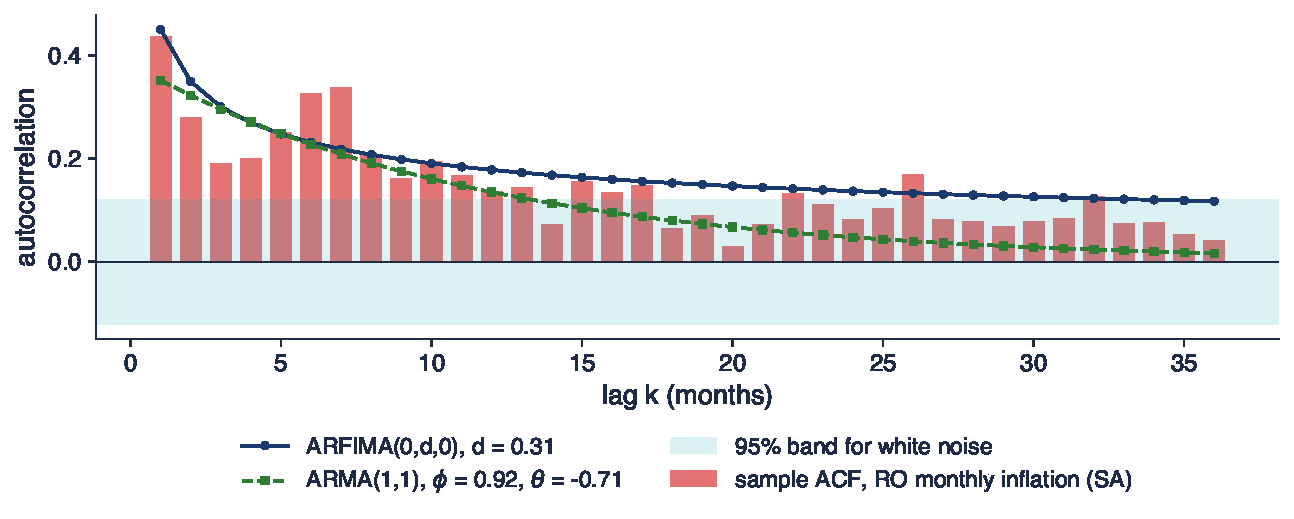
\includegraphics[width=0.97\textwidth,height=0.7\textheight,keepaspectratio]{tsa_ch8_arfima_fit.pdf}
\end{center}
\vspace{-0.25cm}
\begin{itemize}
    \item Bare: ACF de selecție; linii: ACF implicată de ARFIMA$(0,d,0)$ și de ARMA(1,1), ambele estimate prin ML exactă
\end{itemize}
\quantlet{TSA\_ch8\_estimation}{\qlurl{TSA_ch8_estimation}}
\end{frame}

\begin{frame}{Interpretarea ACF a modelelor estimate}
\itemsize{\small}
\begin{itemize}
    \item La decalajul 12: în eșantion 0{,}14, ARFIMA 0{,}18, ARMA(1,1) 0{,}14; la decalajul 24: 0{,}08; 0{,}14 și 0{,}05
    \begin{itemize}
        \item cele două modele sînt de acord pentru primul an și diferă pentru al doilea: prognozele lor pe termen lung vor fi diferite
    \end{itemize}
    \item Curba ARFIMA reproduce coada lentă cu un singur parametru; curba ARMA tinde exponențial spre zero
    \item Ajustarea sezonieră contează: un vîrf sezonier aproape de cele mai joase frecvențe ar distorsiona $\hat d$ (\tsachlink{https://danpele.github.io/Time-Series-Analysis/RO/Cursuri/capitol4_sezonalitate_prognoza.pdf}{Capitolul 4})
\end{itemize}
\end{frame}

\begin{frame}{Memoria lungă în douăsprezece serii}
\itemsize{\footnotesize}
\begin{center}
\scriptsize
\begin{tabular}{lrrrrr}
\toprule
\textbf{Seria} & $T$ & $H_{R/S}$ & $H_{DFA}$ & $d_{GPH}$ & $d_{LW}$ (SE) \\
\midrule
Debitul Nilului & 100 & 0{,}83 & 0{,}64 & 0{,}44 & 0{,}40 (0{,}11) \\
Inflația RO, lunară, ajust. & 260 & 0{,}75 & 0{,}84 & 0{,}37 & 0{,}31 (0{,}08) \\
Inflația RO, anuală & 260 & 0{,}96 & 1{,}38 & 1{,}14 & 1{,}00 (0{,}08) \\
Inflația SUA, lunară & 954 & 0{,}83 & 0{,}87 & 0{,}57 & 0{,}55 (0{,}05) \\
Inflația SUA, 1985--2019 & 420 & 0{,}69 & 0{,}59 & 0{,}07 & 0{,}10 (0{,}07) \\
Șomajul SUA & 944 & 0{,}97 & 1{,}27 & 0{,}82 & 0{,}91 (0{,}05) \\
S\&P 500, $r_t$ & 6\,714 & 0{,}53 & 0{,}49 & 0{,}02 & -0{,}01 (0{,}03) \\
S\&P 500, $|r_t|$ & 6\,714 & 0{,}86 & 0{,}95 & 0{,}56 & 0{,}53 (0{,}03) \\
BET, $r_t$ & 6\,670 & 0{,}58 & 0{,}57 & 0{,}16 & 0{,}12 (0{,}03) \\
BET, $|r_t|$ & 6\,670 & 0{,}79 & 0{,}85 & 0{,}40 & 0{,}39 (0{,}03) \\
EUR/RON, $r_t$ & 5\,352 & 0{,}53 & 0{,}52 & -0{,}01 & -0{,}01 (0{,}03) \\
EUR/RON, $|r_t|$ & 5\,352 & 0{,}82 & 0{,}85 & 0{,}38 & 0{,}39 (0{,}03) \\
\bottomrule
\end{tabular}
\end{center}
\begin{itemize}
    \item $m = \lfloor T^{0{,}65}\rfloor$; date: statsmodels, Eurostat, FRED, EODHD, BNR; randamente zilnice din 2000 (EUR/RON din 2005)
\end{itemize}
\end{frame}

\begin{frame}{Interpretarea tabelului}
\itemsize{\small}
\begin{itemize}
    \item Randamente: $d \approx 0$ pentru S\&P 500 (-0{,}01) și EUR/RON (-0{,}01); mic, dar pozitiv pentru BET (0{,}12)
    \begin{itemize}
        \item randamentele absolute: 0{,}53; 0{,}39 și 0{,}39: memorie lungă în volatilitate (secțiunea 6)
    \end{itemize}
    \item Inflația anuală din România: $d \approx$ 1{,}00, față de 0{,}31 pentru rata lunară: rata anuală însumează 12 variații lunare suprapuse
    \begin{itemize}
        \item suprapunerea anulează spectrul la frecvențele folosite de estimator și împinge $\hat d$ spre 1; modelați rata lunară
    \end{itemize}
    \item Șomajul din SUA: $d \approx$ 0{,}91: nestaționar, dar cu revenire la medie; inflația din SUA în 1985--2019: 0{,}10, față de 0{,}55 în 1947--2026
\end{itemize}
\end{frame}

\begin{frame}{Recapitulare: estimarea lui $d$}
\itemsize{\small}
\begin{itemize}
    \item R/S și DFA: pantele unor grafice log--log, instrumente grafice, deplasate în eșantioane mici
    \item GPH și Whittle local: regresii sau verosimilități pe cele mai joase $m$ frecvențe; raportați mai multe valori ale lui $m$
    \item ML exactă și Whittle: eficienți dacă partea ARMA este corectă; memoria scurtă se poate deghiza în $d$
    \item Inflația lunară din România: ARFIMA$(0,d,0)$ cu $\hat d = 0{,}31$ bate ARMA după AIC și BIC
\end{itemize}
\end{frame}


%=============================================================================
\section{Prognoza cu ARFIMA}
%=============================================================================

\begin{frame}{Prognoze din forma AR($\infty$)}
\itemsize{\small}
\begin{itemize}
    \item Un ARFIMA inversabil se poate scrie $\pi(L)(x_t - \mu) = \varepsilon_t$, cu $\pi(L) = \phi(L)(1-L)^d/\theta(L) = \sum_k\pi_kL^k$
    \begin{itemize}
        \item un pas: $\hat x_{T+1} = \mu - \sum_{k=1}^{T}\pi_k(x_{T+1-k} - \mu)$; $h$ pași: aceeași recurență, cu prognoze în locul valorilor necunoscute
    \end{itemize}
    \item Exemplu, ARFIMA$(0;\ 0{,}4;\ 0)$: $-\pi_k = 0{,}4;\ 0{,}12;\ 0{,}064;\ 0{,}042;\ \dots$
    \begin{itemize}
        \item $\hat x_{T+1} - \mu = 0{,}4(x_T - \mu) + 0{,}12(x_{T-1} - \mu) + 0{,}064(x_{T-2} - \mu) + \dots$: contează toată istoria
        \item un AR(1) folosește doar $x_T$; după o perioadă lungă peste medie, prognoza ARFIMA rămîne mai sus, mai mult timp
    \end{itemize}
    \item Prognozele revin la $\mu$ hiperbolic; varianța erorii de prognoză $\sigma^2\sum_{j<h}\psi_j^2$ crește lent spre $\gamma(0)$ \refRay
\end{itemize}
\end{frame}

\begin{frame}{Inflația din SUA: prognoze ARFIMA și AR}
\itemsize{\footnotesize}
\begin{center}
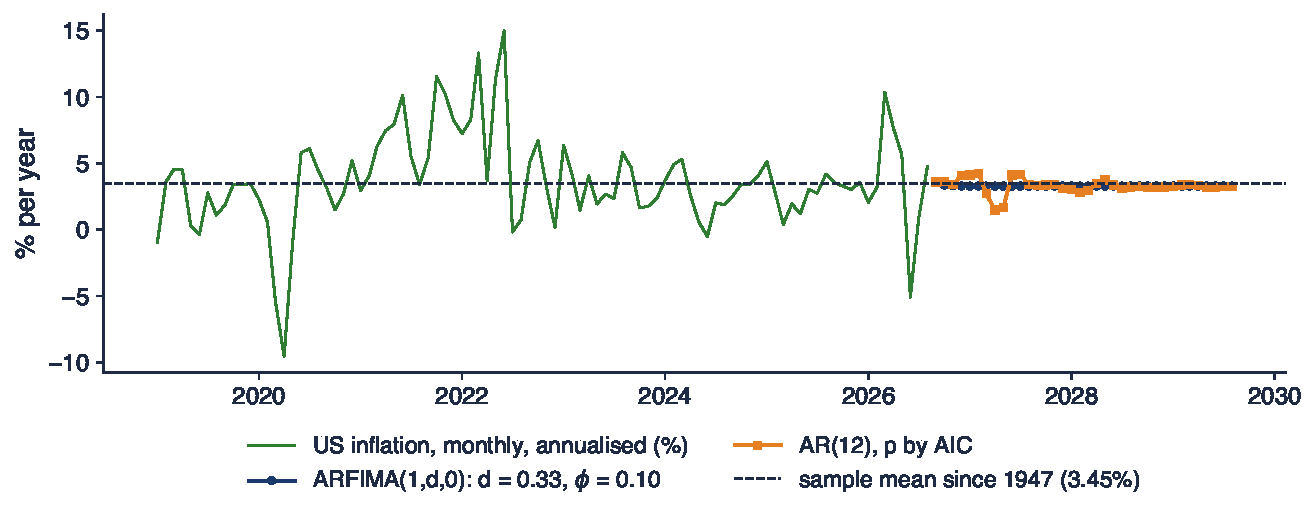
\includegraphics[width=0.97\textwidth,height=0.7\textheight,keepaspectratio]{tsa_ch8_forecast_path.pdf}
\end{center}
\vspace{-0.25cm}
\begin{itemize}
    \item Inflația lunară IPC din SUA, anualizată, $T = 954$ de luni pînă în august 2026; ARFIMA(1,$d$,0) estimat prin Whittle; AR($p$) cu $p$ ales după AIC; 36 de luni înainte
\end{itemize}
\quantlet{TSA\_ch8\_forecasting}{\qlurl{TSA_ch8_forecasting}}
\end{frame}

\begin{frame}{Interpretarea celor două prognoze}
\itemsize{\small}
\begin{itemize}
    \item ARFIMA: $\hat d = 0{,}33$, $\hat\phi = 0{,}10$; AR: $p = 12$ decalaje, numărul maxim permis
    \begin{itemize}
        \item AR are nevoie de un an de decalaje pentru a imita ce face $d$ cu un singur parametru
    \end{itemize}
    \item Media ultimelor 12 luni 3{,}65\%; prognozele: 3{,}62\% și 3{,}59\% luna viitoare, 3{,}28\% și 3{,}38\% peste un an, 3{,}29\% și 3{,}26\% peste trei ani
    \begin{itemize}
        \item ambele se apropie de media pe termen lung 3{,}45\%; traiectoriile diferă puțin, deoarece AR(12) poartă deja o memorie lungă
    \end{itemize}
    \item Dacă media pe termen lung din 1947--2026 este ancora potrivită azi este o întrebare despre regimuri, nu despre $d$
\end{itemize}
\end{frame}

\begin{frame}{Îmbunătățește memoria lungă prognozele?}
\itemsize{\footnotesize}
\begin{center}
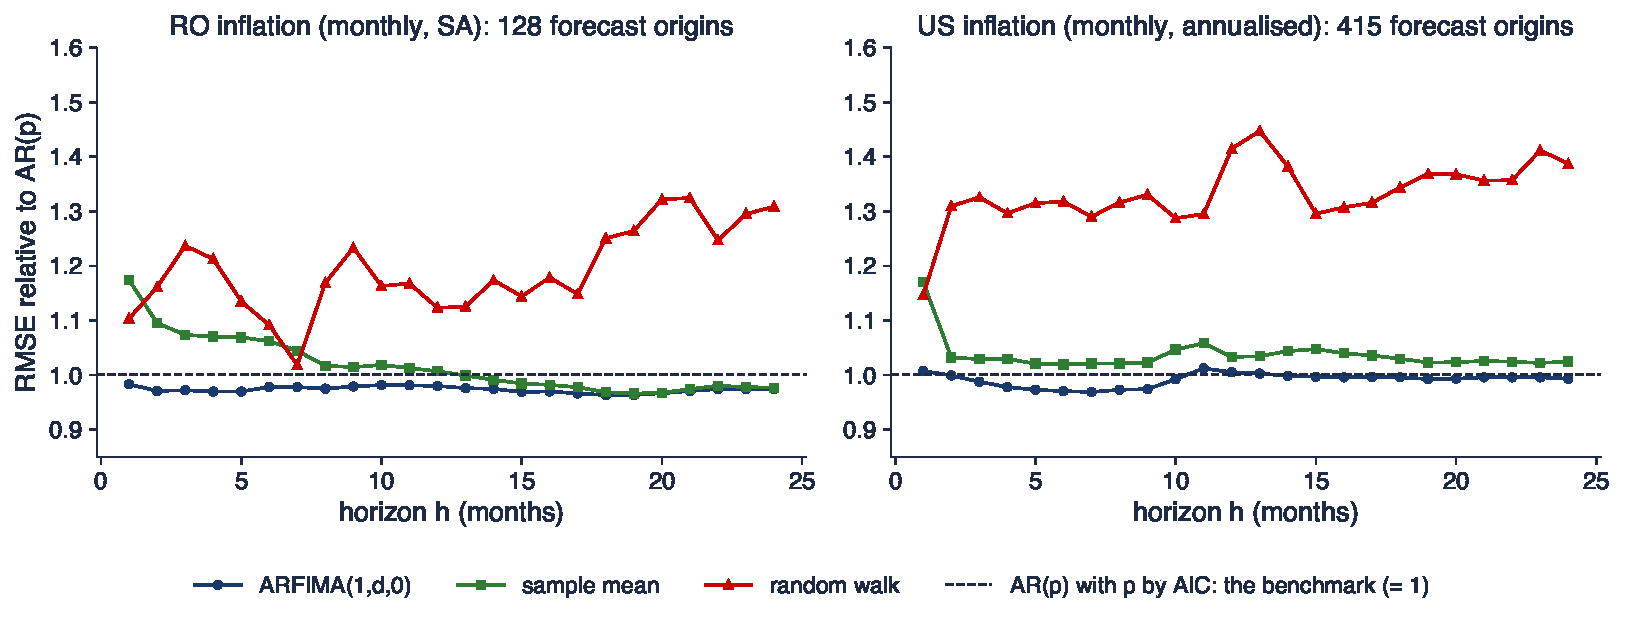
\includegraphics[width=0.97\textwidth,height=0.7\textheight,keepaspectratio]{tsa_ch8_forecast.pdf}
\end{center}
\vspace{-0.25cm}
\begin{itemize}
    \item În afara eșantionului, fereastră extinsă: România 128 de origini (ianuarie 2014--august 2024), ajustare sezonieră în fiecare fereastră; Statele Unite 415 de origini (ianuarie 1990--iulie 2024). RMSE relativ la AR($p$); sub 1: mai bun
\end{itemize}
\quantlet{TSA\_ch8\_forecasting}{\qlurl{TSA_ch8_forecasting}}
\end{frame}

\begin{frame}{Interpretarea comparației prognozelor}
\itemsize{\small}
\begin{itemize}
    \item România: ARFIMA bate AR la toate orizonturile, cu 2--4\% (raportul 0{,}983 la o lună, 0{,}980 la 12, 0{,}974 la 24)
    \begin{itemize}
        \item RMSE la 12 luni: ARFIMA 0{,}53, AR 0{,}54, media 0{,}54, mers aleator 0{,}61 (pp pe lună)
    \end{itemize}
    \item Statele Unite: rapoarte între 0{,}970 și 1{,}005: practic egalitate cu un AR($p$) bogat
    \begin{itemize}
        \item mersul aleator este mult mai slab la toate orizonturile de peste o lună
    \end{itemize}
    \item Memoria lungă aduce cîștiguri modeste, dar constante; erorile mari provin din schimbări de regim (2008, 2021--2022) pe care niciun model liniar nu le anticipează; testați cîștigurile cu Diebold--Mariano (\tsachlink{https://danpele.github.io/Time-Series-Analysis/RO/Cursuri/capitol4_sezonalitate_prognoza.pdf}{Capitolul 4})
\end{itemize}
\end{frame}

\begin{frame}{Recapitulare: prognoza cu ARFIMA}
\itemsize{\small}
\begin{itemize}
    \item Prognoze din ponderile AR($\infty$) $\pi_k$: contează toată istoria
    \item Revenire hiperbolică la medie; incertitudinea prognozei crește lent
    \item Inflația: cîștiguri mici față de AR în România, egalitate în Statele Unite
\end{itemize}
\end{frame}


%=============================================================================
\section{Memoria lungă a volatilității}
%=============================================================================

\begin{frame}{Studiu de caz: Ding, Granger și Engle (1993)}
\itemsize{\small}
\begin{columns}[T]
\begin{column}{0.38\textwidth}
\centering

\includegraphics[height=0.44\textheight]{ch5_robert_engle_2022.jpg}\\[1mm]
\imgcap{Robert F. Engle, Premiul Nobel 2003, împreună cu Clive Granger}
\imgcredit{https://commons.wikimedia.org/wiki/File:0603-Kraneshares_KRBN-RobertEngle-JonDemske-16_(cropped).jpg}{Foto: Jon Demske (2022); CC BY-SA 4.0; Wikimedia Commons}
\end{column}
\begin{column}{0.6\textwidth}
\begin{itemize}
    \item \refDGE: randamentele zilnice S\&P 500, 1928--1991
    \begin{itemize}
        \item randamentele sînt aproape necorelate, dar $|r_t|^\delta$ este autocorelat pe mii de decalaje, cel mai puternic pentru $\delta \approx 1$
        \item „proprietatea de memorie lungă” a randamentelor bursiere: memoria stă în mărime, nu în semn
    \end{itemize}
    \item Un GARCH(1,1) (\tsachlink{https://danpele.github.io/Time-Series-Analysis/RO/Cursuri/capitol5_volatilitate_conditionata_garch.pdf}{Capitolul 5}) implică autocorelații ale lui $r_t^2$ care scad ca $(\alpha + \beta)^k$: exponențial
    \item Rezultatul a dus la FIGARCH \refBBM\ și, cu date de înaltă frecvență, la modelele de volatilitate realizată \refABDL, \refCorsi
\end{itemize}
\end{column}
\end{columns}
\end{frame}

\begin{frame}{Randamente, randamente absolute și pătrate}
\itemsize{\footnotesize}
\begin{center}
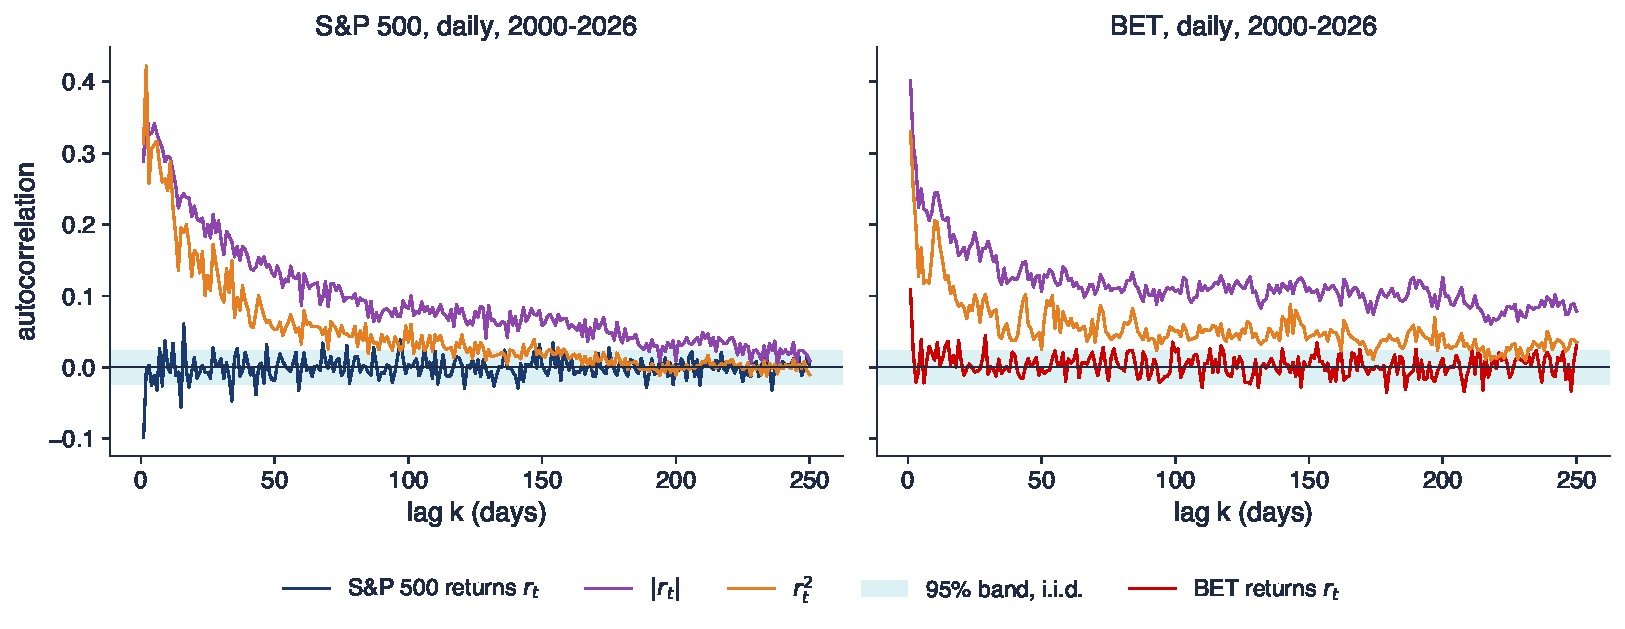
\includegraphics[width=0.97\textwidth,height=0.7\textheight,keepaspectratio]{tsa_ch8_vol_acf.pdf}
\end{center}
\vspace{-0.25cm}
\begin{itemize}
    \item Randamentele logaritmice zilnice ale S\&P 500 ($T = 6\,714$) și BET ($T = 6\,670$), 2000--2026; ACF pînă la decalajul 250 (un an bursier); zona colorată: $\pm 1{,}96/\sqrt T$
\end{itemize}
\quantlet{TSA\_ch8\_volatility\_memory}{\qlurl{TSA_ch8_volatility_memory}}
\end{frame}

\begin{frame}{Interpretarea ACF a volatilității}
\itemsize{\small}
\begin{itemize}
    \item S\&P 500: $|r_t|$ are $\hat\rho = 0{,}29$ la decalajul 1 și încă 0{,}08 la decalajul 100; 227 din 250 de decalaje deasupra benzii
    \begin{itemize}
        \item BET: 0{,}40 la decalajul 1, 0{,}08 la decalajul 250, 250 din 250 deasupra benzii
    \end{itemize}
    \item $|r_t|$ este mai persistent decît $r_t^2$, ca în \refDGE; pătratele sînt dominate de cîteva zile de crah
    \begin{itemize}
        \item Whittle local pentru $|r_t|$: 0{,}53 (S\&P 500), 0{,}39 (BET); după o permutare aleatoare a zilelor: 0{,}00 și -0{,}02
    \end{itemize}
    \item Permutarea păstrează distribuția și distruge ordinea: memoria se află în succesiunea zilelor calme și agitate, nu în cozile groase
\end{itemize}
\end{frame}

\begin{frame}{Volatilitatea realizată}
\itemsize{\small}
\begin{itemize}
    \item \textbf{Varianța realizată} a lunii $m$: $RV_m = \sum_{t \in m} r_t^2$, suma pătratelor randamentelor zilnice din lună \refABDL
    \begin{itemize}
        \item volatilitatea realizată $\sqrt{RV_m}$ măsoară volatilitatea lunii $m$ aproape fără model; cu date intrazilnice aceeași idee dă un RV zilnic
    \end{itemize}
    \item Modelăm $\log\sqrt{RV_m}$: logaritmul aduce distribuția aproape de distribuția Normală și elimină restricția de pozitivitate
    \begin{itemize}
        \item faptul stilizat din \refABDL: logaritmul RV este bine descris de un model cu memorie lungă, cu $d \approx 0{,}4$
    \end{itemize}
    \item Spre deosebire de $|r_t|$, $\log\sqrt{RV_m}$ este o măsură precisă: zgomotul zilelor individuale se compensează în cadrul lunii
\end{itemize}
\end{frame}

\begin{frame}{Volatilitatea realizată lunară: ARFIMA sau ARMA?}
\itemsize{\footnotesize}
\begin{center}
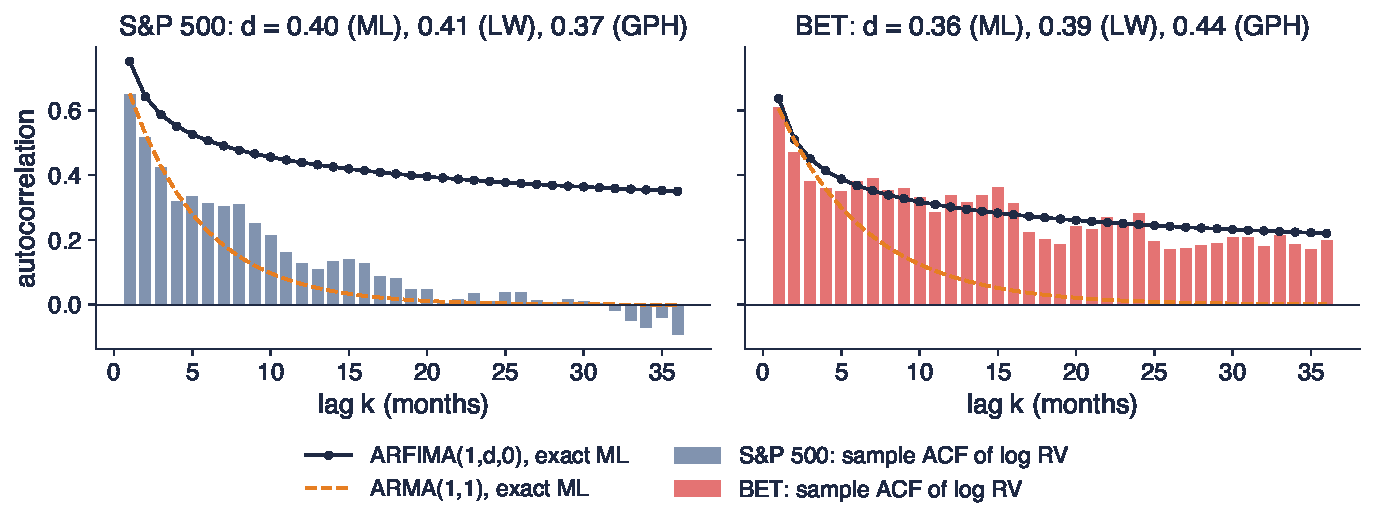
\includegraphics[width=0.97\textwidth,height=0.7\textheight,keepaspectratio]{tsa_ch8_rv.pdf}
\end{center}
\vspace{-0.25cm}
\begin{itemize}
    \item Logaritmul volatilității realizate lunare din randamentele zilnice, 321 de luni (2000--2026); linii: ACF a modelelor ARFIMA(1,$d$,0) și ARMA(1,1), ambele prin ML exactă
\end{itemize}
\quantlet{TSA\_ch8\_volatility\_memory}{\qlurl{TSA_ch8_volatility_memory}}
\end{frame}

\begin{frame}{Interpretarea volatilității realizate}
\itemsize{\small}
\begin{itemize}
    \item Toți estimatorii sînt de acord: $d$ între 0,36 și 0,47 pentru ambele piețe (ML 0{,}40 și 0{,}36)
    \begin{itemize}
        \item BET: ARFIMA reproduce coada lentă (decalajul 24: în eșantion 0{,}28) și cîștigă după BIC (343{,}9 față de 355{,}4 pentru ARMA(1,1))
    \end{itemize}
    \item S\&P 500: ACF de selecție se stinge după aproximativ 20 de luni; ARMA(1,1) cu $\phi = 0{,}81$ se potrivește la fel de bine (BIC 294{,}4 față de 295{,}9)
    \begin{itemize}
        \item cu 27 de ani de date, memoria lungă și un ARMA persistent sînt greu de deosebit
    \end{itemize}
    \item ACF de selecție a unei serii cu memorie lungă este deplasată în jos (media de selecție absoarbe o parte din componenta lentă): judecați modelele după verosimilitate, nu din ochi
\end{itemize}
\end{frame}

\begin{frame}{FIGARCH și HAR}
\itemsize{\small}
\begin{itemize}
    \item \textbf{FIGARCH}$(1,d,1)$ \refBBM: scriem GARCH(1,1) ca ARMA(1,1) în $\varepsilon_t^2$ și aplicăm $(1-L)^d$:
    \begin{itemize}
        \item $\sigma_t^2 = \omega + \beta\sigma_{t-1}^2 + \bigl[1 - \beta L - (1 - \phi L)(1-L)^d\bigr]\varepsilon_t^2 = \omega^* + \sum_{k\ge1}\lambda_k\varepsilon_{t-k}^2$
        \item ponderile ARCH($\infty$) $\lambda_k$ scad ca $k^{-1-d}$; $d = 0$: GARCH, $d = 1$: IGARCH
    \end{itemize}
    \item \textbf{HAR} (model autoregresiv heterogen) \refCorsi: $RV_{t+1} = c + \beta_d RV_t + \beta_w \overline{RV}_{t-4:t} + \beta_m \overline{RV}_{t-21:t} + u_{t+1}$
    \begin{itemize}
        \item medii zilnice, săptămînale și lunare: participanți cu trei orizonturi; estimat prin OLS
        \item nu este un model cu memorie lungă, ci trei trepte care imită o lege de putere pe orizonturile relevante
    \end{itemize}
    \item Ambele răspund unei slăbiciuni a modelului GARCH din \tsachlink{https://danpele.github.io/Time-Series-Analysis/RO/Cursuri/capitol5_volatilitate_conditionata_garch.pdf}{Capitolul 5}: în GARCH șocurile volatilității se sting prea repede
\end{itemize}
\end{frame}

\begin{frame}{FIGARCH comparat cu GARCH; HAR comparat cu $(1-L)^d$}
\itemsize{\footnotesize}
\begin{center}
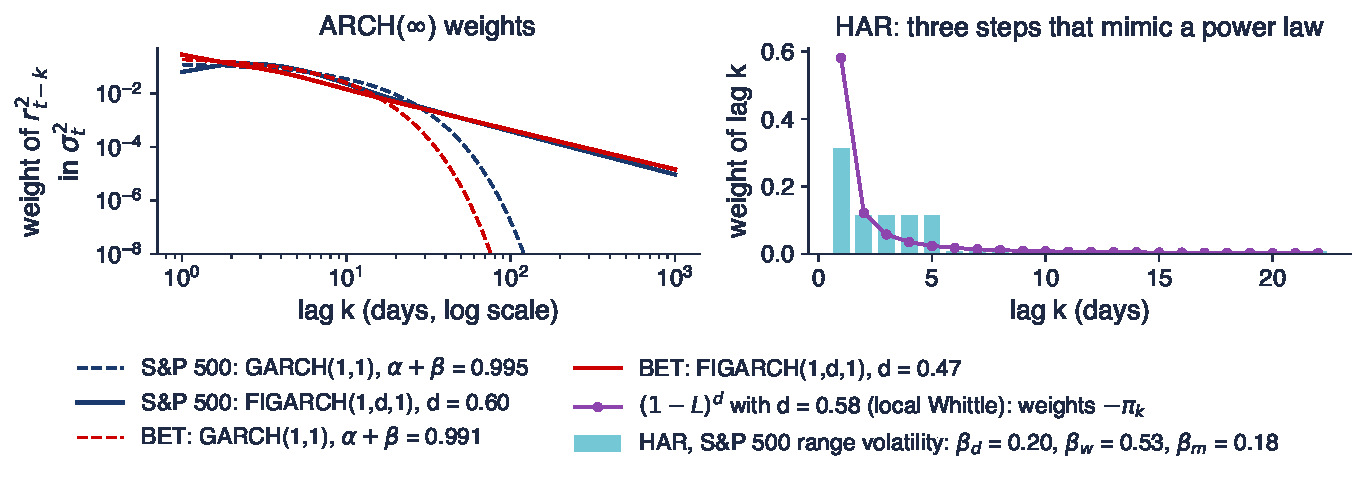
\includegraphics[width=0.97\textwidth,height=0.7\textheight,keepaspectratio]{tsa_ch8_vol_models.pdf}
\end{center}
\vspace{-0.25cm}
\begin{itemize}
    \item Stînga: ponderile ARCH($\infty$) ale GARCH(1,1) și FIGARCH(1,$d$,1), erori Student $t$, randamente zilnice 2000--2026 (\texttt{arch}). Dreapta: HAR pentru volatilitatea zilnică pe baza amplitudinii S\&P 500 (estimatorul Parkinson, din prețurile maxime și minime)
\end{itemize}
\quantlet{TSA\_ch8\_volatility\_memory}{\qlurl{TSA_ch8_volatility_memory}}
\end{frame}

\begin{frame}{Interpretarea modelelor FIGARCH și HAR}
\itemsize{\small}
\begin{itemize}
    \item FIGARCH: $\hat d = 0{,}60$ (S\&P 500) și 0{,}47 (BET); BIC scade cu 34 și 71 față de GARCH
    \begin{itemize}
        \item ponderea unui șoc de acum 100 de zile în varianța de azi: GARCH $1{,}6 \cdot 10^{-7}$, FIGARCH $3{,}9 \cdot 10^{-4}$ (S\&P 500): cu trei ordine de mărime mai mult
    \end{itemize}
    \item GARCH obține persistența prin $\alpha + \beta = 0{,}995$, aproape de 1: rezultatul aproape IGARCH din \tsachlink{https://danpele.github.io/Time-Series-Analysis/RO/Cursuri/capitol5_volatilitate_conditionata_garch.pdf}{Capitolul 5} este un simptom al memoriei lungi
    \begin{itemize}
        \item HAR: $\hat\beta_d = 0{,}20$, $\hat\beta_w = 0{,}53$, $\hat\beta_m = 0{,}18$; componenta săptămînală domină
    \end{itemize}
    \item Treptele HAR (0{,}31 la decalajul 1, 0{,}11 la decalajele 2--5, 0{,}008 la decalajele 6--22) urmează ponderile hiperbolice ale lui $(1-L)^d$, cu $d = 0{,}58$ din estimatorul Whittle local
\end{itemize}
\end{frame}

\begin{frame}{Recapitulare: memoria lungă a volatilității}
\itemsize{\small}
\begin{itemize}
    \item Randamente: $d \approx 0$; randamente absolute și volatilitate realizată: $d \approx 0{,}4$
    \item Testul permutării: memoria stă în ordinea zilelor, nu în distribuție
    \item FIGARCH: ponderi ARCH($\infty$) hiperbolice; HAR: o aproximare simplă prin OLS
\end{itemize}
\end{frame}


%=============================================================================
\section{Memoria lungă aparentă}
%=============================================================================

\begin{frame}{Rupturile și regimurile seamănă cu memoria lungă}
\itemsize{\small}
\begin{itemize}
    \item O schimbare de nivel adaugă o componentă lentă, în trepte: frecvențele joase cîștigă putere, iar ACF de selecție scade lent
    \begin{itemize}
        \item același mecanism care face ca o serie cu ruptură să pară cu rădăcină unitară (Perron, \tsachlink{https://danpele.github.io/Time-Series-Analysis/RO/Cursuri/capitol3_radacini_unitare_modele_arima.pdf}{Capitolul 3})
    \end{itemize}
    \item \refDI: o medie cu schimbări de regim de tip Markov, cu schimbări rare, este „echivalentă observațional” cu memoria lungă
    \begin{itemize}
        \item cu cît sînt mai puține schimbări într-un eșantion de lungime $T$, cu atît seria seamănă mai mult cu $I(d)$
        \item modelele cu schimbare de regim sînt tema \tsachlink{https://danpele.github.io/Time-Series-Analysis/RO/Cursuri/capitol10_spatiul_starilor_kalman_markov_switching.pdf}{Capitolului 10}
    \end{itemize}
    \item \refGH: rupturile ocazionale explică o mare parte din memoria lungă a randamentelor absolute S\&P 500
\end{itemize}
\end{frame}

\begin{frame}{Memorie scurtă care pare lungă}
\itemsize{\footnotesize}
\begin{center}
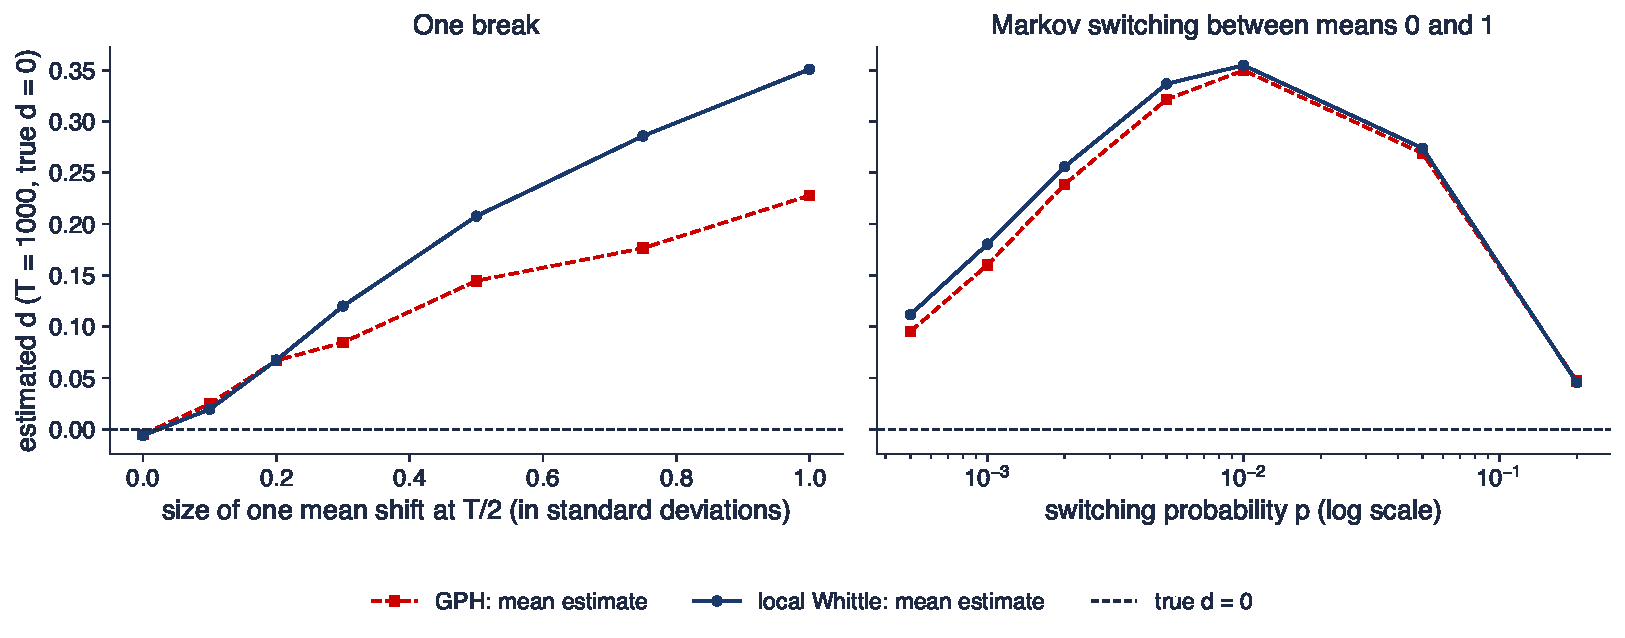
\includegraphics[width=0.97\textwidth,height=0.7\textheight,keepaspectratio]{tsa_ch8_spurious.pdf}
\end{center}
\vspace{-0.25cm}
\begin{itemize}
    \item 200 de eșantioane de $T = 1000$, $d = 0$ în realitate. Stînga: zgomot $N(0,1)$ cu o singură schimbare a mediei la $T/2$; dreapta: zgomot $N(0,1)$ plus o medie care trece între 0 și 1 cu probabilitatea $p$ în fiecare perioadă
\end{itemize}
\quantlet{TSA\_ch8\_spurious\_memory}{\qlurl{TSA_ch8_spurious_memory}}
\end{frame}

\begin{frame}{Interpretarea memoriei aparente}
\itemsize{\small}
\begin{itemize}
    \item O singură schimbare de o jumătate de abatere standard dă deja $\hat d = 0{,}21$ (Whittle local); o schimbare de o abatere standard dă 0{,}35
    \begin{itemize}
        \item ruptura se vede greu cu ochiul în date zgomotoase, dar estimatorul raportează o memorie lungă moderată
    \end{itemize}
    \item Schimbări de regim: cu $p = 0{,}01$ (aproximativ 10 schimbări) $\hat d = 0{,}35$; cu $p = 0{,}2$ (schimbări frecvente) $\hat d = 0{,}05$
    \begin{itemize}
        \item regimurile rare par memorie, cele frecvente se compensează și dau memorie scurtă
    \end{itemize}
    \item Un $\hat d$ semnificativ este compatibil atît cu memoria lungă, cît și cu rupturile: este nevoie de alte dovezi pentru a decide
\end{itemize}
\end{frame}

\begin{frame}{Nilul în 1898: memorie sau ruptură?}
\itemsize{\footnotesize}
\begin{center}
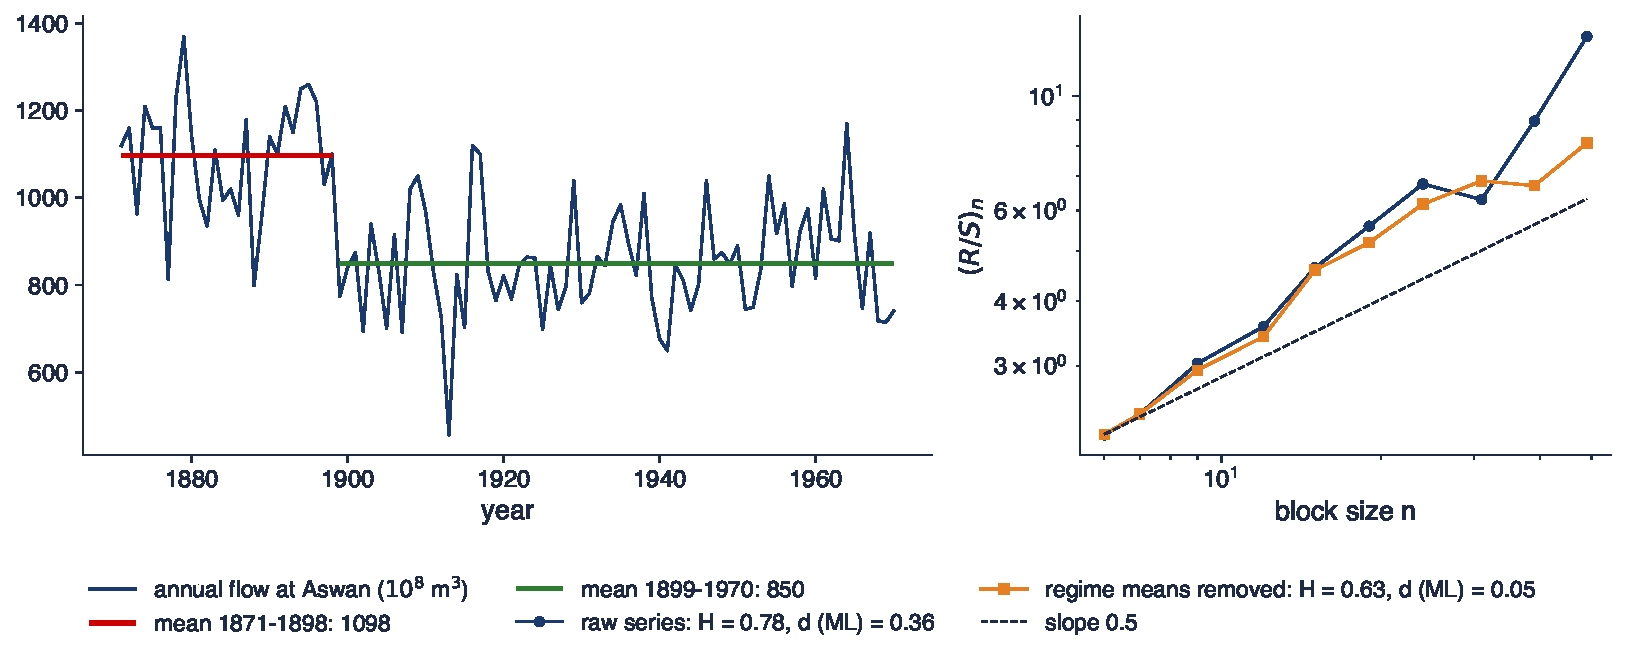
\includegraphics[width=0.97\textwidth,height=0.7\textheight,keepaspectratio]{tsa_ch8_nile_break.pdf}
\end{center}
\vspace{-0.25cm}
\begin{itemize}
    \item Stînga: debitul, cu mediile dinainte și de după 1898, punctul de schimbare din \refCobb{} (primul baraj de la Aswan a fost finalizat în 1902); dreapta: graficul R/S pentru seria brută și pentru seria fără cele două medii de regim
\end{itemize}
\quantlet{TSA\_ch8\_spurious\_memory}{\qlurl{TSA_ch8_spurious_memory}}
\end{frame}

\begin{frame}{Interpretarea rupturii Nilului}
\itemsize{\small}
\begin{itemize}
    \item Media scade de la 1098 la 850 ($-$23\%) după 1898
    \begin{itemize}
        \item seria brută: $\hat d = 0{,}36$ (ML exactă, SE 0{,}07), Whittle local 0{,}40, R/S $H = 0{,}78$
    \end{itemize}
    \item Fără mediile de regim: $\hat d = 0{,}05$ (SE 0{,}10), Whittle local -0{,}17; $\hat\rho(1)$ scade de la 0{,}50 la 0{,}16
    \begin{itemize}
        \item pentru acești 100 de ani o singură ruptură explică aproape toată memoria
    \end{itemize}
    \item Dovezile lui Hurst proveneau din înregistrări mult mai lungi (nilometrul de la Roda, din secolul al VII-lea); lecția: testați rupturile înainte de a interpreta $d$
\end{itemize}
\end{frame}

\begin{frame}{Este memoria stabilă în timp?}
\itemsize{\footnotesize}
\begin{center}
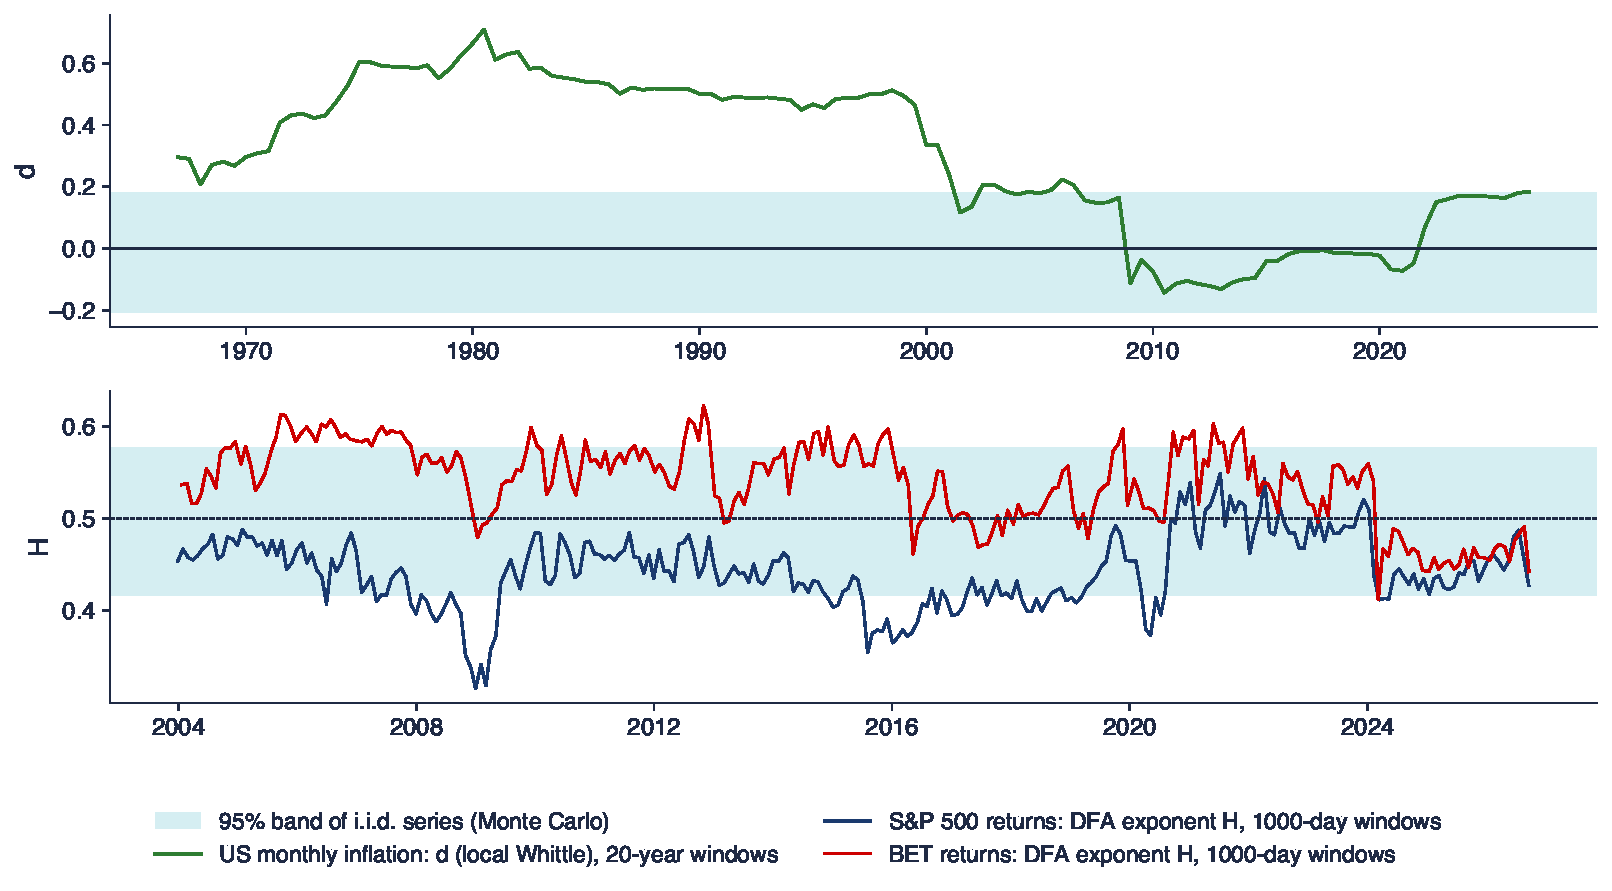
\includegraphics[width=0.97\textwidth,height=0.7\textheight,keepaspectratio]{tsa_ch8_rolling.pdf}
\end{center}
\vspace{-0.25cm}
\begin{itemize}
    \item Sus: $\hat d$ Whittle local pentru inflația lunară din SUA, pe ferestre mobile de 20 de ani (datate la sfîrșitul ferestrei); jos: exponentul DFA al randamentelor zilnice S\&P 500 și BET, pe ferestre de 1000 de zile mutate cu 21 de zile; zona colorată: benzi Monte Carlo de 95\% pentru serii i.i.d. \refWeron
\end{itemize}
\quantlet{TSA\_ch8\_spurious\_memory}{\qlurl{TSA_ch8_spurious_memory}}
\end{frame}

\begin{frame}{Interpretarea estimărilor pe ferestre mobile}
\itemsize{\small}
\begin{itemize}
    \item Inflația din SUA: $\hat d$ atinge 0{,}71 în fereastra care se încheie în iulie 1980 (Marea Inflație și dezinflația Volcker) și coboară la -0{,}14 (iulie 2010)
    \begin{itemize}
        \item în anii calmi ai țintirii inflației $d$ se află în banda fără memorie [-0{,}21; 0{,}18]; puseul din 2021--2022 îl readuce la 0{,}18
    \end{itemize}
    \item Randamentele: exponentul S\&P 500 stă mai ales sub 0,5 (minimum 0{,}32, decembrie 2008); BET depășește banda în 24\% din ferestre
    \begin{itemize}
        \item o piață mai puțin lichidă arată o anumită persistență a randamentelor, care slăbește în ultimii ani
    \end{itemize}
    \item Estimarea pe tot eșantionul pentru SUA (0,55) amestecă regimuri: o memorie care apare și dispare odată cu regimurile monetare semnalează rupturi, nu un $d$ constant
\end{itemize}
\end{frame}

\begin{frame}{Verificări împotriva memoriei lungi aparente}
\itemsize{\small}
\begin{itemize}
    \item Reprezentați seria grafic și testați rupturile (\tsachlink{https://danpele.github.io/Time-Series-Analysis/RO/Cursuri/capitol3_radacini_unitare_modele_arima.pdf}{Capitolul 3}: Zivot--Andrews, Bai--Perron); reestimați $d$ pe subeșantioane și după eliminarea mediilor de regim
    \item Raportați $\hat d$ pentru mai multe lățimi de bandă $m$; o valoare care se prăbușește cînd $m$ se schimbă este fragilă
    \item Comparați ARFIMA cu ARMA și cu modele cu schimbare de regim după verosimilitate și prin prognoze în afara eșantionului (\tsachlink{https://danpele.github.io/Time-Series-Analysis/RO/Cursuri/capitol10_spatiul_starilor_kalman_markov_switching.pdf}{Capitolul 10})
    \item Folosiți testul permutării și benzi Monte Carlo construite pentru aceeași lungime a eșantionului
    \item Evitați datele suprapuse (inflația anuală, sumele pe ferestre mobile): ele creează putere artificială la frecvențele joase
\end{itemize}
\end{frame}

\begin{frame}{Recapitulare: memoria lungă aparentă}
\itemsize{\small}
\begin{itemize}
    \item Rupturile și schimbările rare de regim produc $\hat d > 0$ în serii cu memorie scurtă
    \item Nilul: o singură ruptură în 1898 explică cea mai mare parte a memoriei din 1871--1970
    \item Inflația din SUA: $d$ se schimbă odată cu regimul monetar
\end{itemize}
\end{frame}


%=============================================================================
\section{O trimitere: cointegrarea fracționară}
%=============================================================================

\begin{frame}{Cointegrarea fracționară}
\itemsize{\small}
\begin{itemize}
    \item \tsachlink{https://danpele.github.io/Time-Series-Analysis/RO/Cursuri/capitol7_cointegrare_vecm.pdf}{Capitolul 7}: două serii $I(1)$ sînt cointegrate dacă o combinație $y_t - \beta x_t$ este $I(0)$
    \begin{itemize}
        \item \textbf{cointegrare fracționară}: $x_t, y_t \sim I(d)$ și $y_t - \beta x_t \sim I(d - b)$, cu $0 < b \le d$
        \item eroarea de echilibru poate avea ea însăși memorie lungă: abaterile de la echilibru sînt corectate, dar lent
    \end{itemize}
    \item Exemplu: paritatea puterii de cumpărare \refCL: cursul real revine la paritate cu un $d$ între 0 și 1
    \begin{itemize}
        \item testele Engle--Granger și Johansen din \tsachlink{https://danpele.github.io/Time-Series-Analysis/RO/Cursuri/capitol7_cointegrare_vecm.pdf}{Capitolul 7} presupun $b = 1$ și pot rata o astfel de ajustare lentă
    \end{itemize}
    \item Dincolo de acest curs; un proiect natural: estimați $d$ al reziduului unei regresii de cointegrare cu estimatorul Whittle local
\end{itemize}
\end{frame}


%=============================================================================
\section{Contribuția posibilă a AI}
%=============================================================================

\begin{frame}{Contribuția posibilă a AI}
\itemsize{\small}
\begin{itemize}
    \item \textbf{Cod}: o primă versiune a diferențierii fracționare, a estimatorilor GPH și Whittle local, a unei verosimilități ARFIMA
    \item \textbf{Explicații}: o a doua explicație a periodogramei, a compromisului lățimii de bandă, a legăturii $H = d + 1/2$
    \item \textbf{Explorare}: $d$ pentru inflația multor țări sau volatilitatea multor active, cu subeșantioane și lățimi de bandă diferite
    \item Exemplu de prompt
    \begin{itemize}
        \item \aiprompt{Write Python code that downloads Romanian monthly HICP (Eurostat prc\_hicp\_minr), computes the monthly inflation rate, removes the monthly means, estimates d with GPH and local Whittle for bandwidths T\^{}0.5 to T\^{}0.8, fits ARFIMA(p,d,q) by exact Gaussian maximum likelihood and compares it with ARMA(1,1) by BIC.}
    \end{itemize}
\end{itemize}
\end{frame}

\begin{frame}{Verificări necesare}
\itemsize{\small}
\begin{itemize}
    \item Biblioteca: \texttt{statsmodels} nu are o clasă ARFIMA; un răspuns AI care folosește una a inventat-o
    \item Semnul și scala: GPH regresează pe $-\log(4\sin^2(\lambda/2))$, deci panta este $d$, nu $-2d$; R/S și DFA dau $H$, nu $d$
    \item Intervalul: verosimilitatea unui ARFIMA staționar cere $d < 0{,}5$; diferențiați întîi dacă $\hat d$ este aproape de 0,5 sau peste
    \item Simulați o serie cu $d$ cunoscut și verificați că codul îl regăsește
    \item Rupturile, sezonalitatea și datele suprapuse, înainte de orice afirmație despre memoria lungă
    \item Fiecare referință citată: trebuie să existe; verificați DOI-ul
\end{itemize}
\end{frame}


%=============================================================================
\section{Rezumat}
%=============================================================================

\begin{frame}{Idei de reținut}
\itemsize{\small}
\begin{itemize}
    \item Memoria lungă: descreștere hiperbolică a ACF $\rho(k) \sim Ck^{2d-1}$ și un pol spectral la zero; memoria ARMA este exponențială
    \item $(1-L)^d$ cu $d$ real; ARFIMA$(p,d,q)$ separă memoria pe termen lung ($d$) de dinamica pe termen scurt (ARMA)
    \item Staționar pentru $d < 1/2$, inversabil pentru $d > -1/2$, cu revenire la medie pentru $d < 1$; $H = d + 1/2$
    \item Estimați $d$ cu mai multe metode și lățimi de bandă; preferați comparațiile cu ARMA pe baza verosimilității
    \item Inflația și volatilitatea au memorie lungă; randamentele nu; rupturile și regimurile o pot imita
\end{itemize}
\end{frame}

\begin{frame}{Formule de reținut}
\itemsize{\small}
{\renewcommand{\arraystretch}{1.35}\begin{center}
\scriptsize
\begin{tabular}{ll}
\toprule
\textbf{Mărimea} & \textbf{Formula} \\
\midrule
ARFIMA$(p,d,q)$ & $\phi(L)(1-L)^d(x_t - \mu) = \theta(L)\varepsilon_t$ \\
Ponderile lui $(1-L)^d$ & $\pi_0 = 1$, \quad $\pi_k = \pi_{k-1}(k - 1 - d)/k$ \\
ACF pentru ARFIMA$(0,d,0)$ & $\rho(1) = d/(1-d)$, \quad $\rho(k) = \rho(k-1)(k-1+d)/(k-d) \sim Ck^{2d-1}$ \\
Spectrul în apropierea lui 0 & $f(\lambda) \sim G\lambda^{-2d}$ \\
GPH & $\log I(\lambda_j) = c + d\,[-\log(4\sin^2(\lambda_j/2))] + u_j$, \quad SE $= \pi/\sqrt{24m}$ \\
Whittle local & $\min_d \log\bigl(\tfrac1m\sum_j\lambda_j^{2d}I(\lambda_j)\bigr) - \tfrac{2d}{m}\sum_j\log\lambda_j$, \quad SE $= 1/(2\sqrt m)$ \\
R/S, DFA & $E(R/S)_n \approx cn^H$, \quad $F(n) \approx cn^H$, \quad $H = d + 1/2$ \\
FIGARCH & $\sigma_t^2 = \omega + \beta\sigma_{t-1}^2 + [1 - \beta L - (1 - \phi L)(1-L)^d]\varepsilon_t^2$ \\
\bottomrule
\end{tabular}
\end{center}
}
\end{frame}

\begin{frame}{Autoevaluare}
\itemsize{\small}
\begin{itemize}
    \item \textbf{Întrebare}: cît sînt $\pi_1$ și $\pi_2$ pentru $(1-L)^{0{,}2}$?
    \begin{itemize}
        \item \textbf{Răspuns}: $\pi_1 = -0{,}2$, $\pi_2 = -0{,}2 \cdot 0{,}8/2 = -0{,}08$
    \end{itemize}
    \item \textbf{Întrebare}: este staționar un ARFIMA$(0;\ 0{,}7;\ 0)$?
    \begin{itemize}
        \item \textbf{Răspuns}: nu ($d \ge 0{,}5$), dar revine la medie; prima ei diferență este ARFIMA$(0;\ -0{,}3;\ 0)$, staționar și antipersistent
    \end{itemize}
    \item \textbf{Întrebare}: GPH dă $\hat d = 0{,}35$ pentru o serie cu o schimbare mare de nivel. Este aceasta o dovadă de memorie lungă?
    \begin{itemize}
        \item \textbf{Răspuns}: nu, prin ea însăși: o ruptură produce aceeași putere la frecvențele joase; reestimați după eliminarea schimbării și pe subeșantioane
    \end{itemize}
    \item Urmează: \tsachlink{https://danpele.github.io/Time-Series-Analysis/RO/Cursuri/capitol9_invatare_automata_serii_timp.pdf}{Capitolul 9}, învățarea automată pentru serii de timp
\end{itemize}
\end{frame}


%=============================================================================
\section{Bibliografie}
%=============================================================================

\begin{frame}{Bibliografie (1/2)}
\itemsize{\tiny}
\begin{itemize}
    \item Andersen, T. G., Bollerslev, T., Diebold, F. X., \& Labys, P. (2003). Modeling and forecasting realized volatility. \textit{Econometrica}, 71(2), 579--625. \href{https://doi.org/10.1111/1468-0262.00418}{doi:10.1111/1468-0262.00418}
    \item Baillie, R. T. (1996). Long memory processes and fractional integration in econometrics. \textit{Journal of Econometrics}, 73(1), 5--59. \href{https://doi.org/10.1016/0304-4076(95)01732-1}{doi:10.1016/0304-4076(95)01732-1}
    \item Baillie, R. T., Bollerslev, T., \& Mikkelsen, H. O. (1996). Fractionally integrated generalized autoregressive conditional heteroskedasticity. \textit{Journal of Econometrics}, 74(1), 3--30. \href{https://doi.org/10.1016/S0304-4076(95)01749-6}{doi:10.1016/S0304-4076(95)01749-6}
    \item Beran, J., Feng, Y., Ghosh, S., \& Kulik, R. (2013). \textit{Long-Memory Processes: Probabilistic Properties and Statistical Methods}. Springer. \href{https://doi.org/10.1007/978-3-642-35512-7}{doi:10.1007/978-3-642-35512-7}
    \item Brockwell, P. J., \& Davis, R. A. (1991). \textit{Time Series: Theory and Methods} (2nd ed.). Springer. \href{https://doi.org/10.1007/978-1-4419-0320-4}{doi:10.1007/978-1-4419-0320-4}
    \item Cheung, Y.-W., \& Lai, K. S. (1993). A fractional cointegration analysis of purchasing power parity. \textit{Journal of Business \& Economic Statistics}, 11(1), 103--112. \href{https://doi.org/10.1080/07350015.1993.10509936}{doi:10.1080/07350015.1993.10509936}
    \item Cobb, G. W. (1978). The problem of the Nile: Conditional solution to a changepoint problem. \textit{Biometrika}, 65(2), 243--251. \href{https://doi.org/10.1093/biomet/65.2.243}{doi:10.1093/biomet/65.2.243}
    \item Corsi, F. (2009). A simple approximate long-memory model of realized volatility. \textit{Journal of Financial Econometrics}, 7(2), 174--196. \href{https://doi.org/10.1093/jjfinec/nbp001}{doi:10.1093/jjfinec/nbp001}
    \item Diebold, F. X., \& Inoue, A. (2001). Long memory and regime switching. \textit{Journal of Econometrics}, 105(1), 131--159. \href{https://doi.org/10.1016/S0304-4076(01)00073-2}{doi:10.1016/S0304-4076(01)00073-2}
    \item Ding, Z., Granger, C. W. J., \& Engle, R. F. (1993). A long memory property of stock market returns and a new model. \textit{Journal of Empirical Finance}, 1(1), 83--106. \href{https://doi.org/10.1016/0927-5398(93)90006-D}{doi:10.1016/0927-5398(93)90006-D}
    \item Fox, R., \& Taqqu, M. S. (1986). Large-sample properties of parameter estimates for strongly dependent stationary Gaussian time series. \textit{The Annals of Statistics}, 14(2), 517--532. \href{https://doi.org/10.1214/aos/1176349936}{doi:10.1214/aos/1176349936}
    \item Geweke, J., \& Porter-Hudak, S. (1983). The estimation and application of long memory time series models. \textit{Journal of Time Series Analysis}, 4(4), 221--238. \href{https://doi.org/10.1111/j.1467-9892.1983.tb00371.x}{doi:10.1111/j.1467-9892.1983.tb00371.x}
    \item Granger, C. W. J., \& Hyung, N. (2004). Occasional structural breaks and long memory with an application to the S\&P 500 absolute stock returns. \textit{Journal of Empirical Finance}, 11(3), 399--421. \href{https://doi.org/10.1016/j.jempfin.2003.03.001}{doi:10.1016/j.jempfin.2003.03.001}
    \item Granger, C. W. J., \& Joyeux, R. (1980). An introduction to long-memory time series models and fractional differencing. \textit{Journal of Time Series Analysis}, 1(1), 15--29. \href{https://doi.org/10.1111/j.1467-9892.1980.tb00297.x}{doi:10.1111/j.1467-9892.1980.tb00297.x}
    \item Graves, T., Gramacy, R., Watkins, N., \& Franzke, C. (2017). A brief history of long memory: Hurst, Mandelbrot and the road to ARFIMA, 1951--1980. \textit{Entropy}, 19(9), 437. \href{https://doi.org/10.3390/e19090437}{doi:10.3390/e19090437}
    \item Hassler, U., \& Wolters, J. (1995). Long memory in inflation rates: International evidence. \textit{Journal of Business \& Economic Statistics}, 13(1), 37--45. \href{https://doi.org/10.1080/07350015.1995.10524577}{doi:10.1080/07350015.1995.10524577}
\end{itemize}
\end{frame}

\begin{frame}{Bibliografie (2/2)}
\itemsize{\tiny}
\begin{itemize}
    \item Hosking, J. R. M. (1981). Fractional differencing. \textit{Biometrika}, 68(1), 165--176. \href{https://doi.org/10.1093/biomet/68.1.165}{doi:10.1093/biomet/68.1.165}
    \item Huang, C., \& Petukhina, A. (2022). \textit{Applied Time Series Analysis and Forecasting with Python}. Springer. \href{https://doi.org/10.1007/978-3-031-13584-2}{doi:10.1007/978-3-031-13584-2}
    \item Hurst, H. E. (1951). Long-term storage capacity of reservoirs. \textit{Transactions of the American Society of Civil Engineers}, 116(1), 770--799. \href{https://doi.org/10.1061/TACEAT.0006518}{doi:10.1061/TACEAT.0006518}
    \item Lo, A. W. (1991). Long-term memory in stock market prices. \textit{Econometrica}, 59(5), 1279--1313. \href{https://doi.org/10.2307/2938368}{doi:10.2307/2938368}
    \item Mandelbrot, B. B., \& Van Ness, J. W. (1968). Fractional Brownian motions, fractional noises and applications. \textit{SIAM Review}, 10(4), 422--437. \href{https://doi.org/10.1137/1010093}{doi:10.1137/1010093}
    \item Mandelbrot, B. B., \& Wallis, J. R. (1968). Noah, Joseph, and operational hydrology. \textit{Water Resources Research}, 4(5), 909--918. \href{https://doi.org/10.1029/WR004i005p00909}{doi:10.1029/WR004i005p00909}
    \item Mandelbrot, B. B., \& Wallis, J. R. (1969). Robustness of the rescaled range R/S in the measurement of noncyclic long run statistical dependence. \textit{Water Resources Research}, 5(5), 967--988. \href{https://doi.org/10.1029/WR005i005p00967}{doi:10.1029/WR005i005p00967}
    \item Peng, C.-K., Buldyrev, S. V., Havlin, S., Simons, M., Stanley, H. E., \& Goldberger, A. L. (1994). Mosaic organization of DNA nucleotides. \textit{Physical Review E}, 49(2), 1685--1689. \href{https://doi.org/10.1103/PhysRevE.49.1685}{doi:10.1103/PhysRevE.49.1685}
    \item Ray, B. K. (1993). Modeling long-memory processes for optimal long-range prediction. \textit{Journal of Time Series Analysis}, 14(5), 511--525. \href{https://doi.org/10.1111/j.1467-9892.1993.tb00161.x}{doi:10.1111/j.1467-9892.1993.tb00161.x}
    \item Robinson, P. M. (1995). Gaussian semiparametric estimation of long range dependence. \textit{The Annals of Statistics}, 23(5), 1630--1661. \href{https://doi.org/10.1214/aos/1176324317}{doi:10.1214/aos/1176324317}
    \item Sowell, F. (1992). Maximum likelihood estimation of stationary univariate fractionally integrated time series models. \textit{Journal of Econometrics}, 53(1--3), 165--188. \href{https://doi.org/10.1016/0304-4076(92)90084-5}{doi:10.1016/0304-4076(92)90084-5}
    \item Velasco, C. (1999). Gaussian semiparametric estimation of non-stationary time series. \textit{Journal of Time Series Analysis}, 20(1), 87--127. \href{https://doi.org/10.1111/1467-9892.00127}{doi:10.1111/1467-9892.00127}
    \item Weron, R. (2002). Estimating long-range dependence: Finite sample properties and confidence intervals. \textit{Physica A}, 312(1--2), 285--299. \href{https://doi.org/10.1016/S0378-4371(02)00961-5}{doi:10.1016/S0378-4371(02)00961-5}
\end{itemize}
\end{frame}

\end{document}
